\documentclass{beamer}\usepackage[]{graphicx}\usepackage[]{color}
%% maxwidth is the original width if it is less than linewidth
%% otherwise use linewidth (to make sure the graphics do not exceed the margin)
\makeatletter
\def\maxwidth{ %
  \ifdim\Gin@nat@width>\linewidth
    \linewidth
  \else
    \Gin@nat@width
  \fi
}
\makeatother

\definecolor{fgcolor}{rgb}{0.345, 0.345, 0.345}
\newcommand{\hlnum}[1]{\textcolor[rgb]{0.686,0.059,0.569}{#1}}%
\newcommand{\hlstr}[1]{\textcolor[rgb]{0.192,0.494,0.8}{#1}}%
\newcommand{\hlcom}[1]{\textcolor[rgb]{0.678,0.584,0.686}{\textit{#1}}}%
\newcommand{\hlopt}[1]{\textcolor[rgb]{0,0,0}{#1}}%
\newcommand{\hlstd}[1]{\textcolor[rgb]{0.345,0.345,0.345}{#1}}%
\newcommand{\hlkwa}[1]{\textcolor[rgb]{0.161,0.373,0.58}{\textbf{#1}}}%
\newcommand{\hlkwb}[1]{\textcolor[rgb]{0.69,0.353,0.396}{#1}}%
\newcommand{\hlkwc}[1]{\textcolor[rgb]{0.333,0.667,0.333}{#1}}%
\newcommand{\hlkwd}[1]{\textcolor[rgb]{0.737,0.353,0.396}{\textbf{#1}}}%

\usepackage{framed}
\makeatletter
\newenvironment{kframe}{%
 \def\at@end@of@kframe{}%
 \ifinner\ifhmode%
  \def\at@end@of@kframe{\end{minipage}}%
  \begin{minipage}{\columnwidth}%
 \fi\fi%
 \def\FrameCommand##1{\hskip\@totalleftmargin \hskip-\fboxsep
 \colorbox{shadecolor}{##1}\hskip-\fboxsep
     % There is no \\@totalrightmargin, so:
     \hskip-\linewidth \hskip-\@totalleftmargin \hskip\columnwidth}%
 \MakeFramed {\advance\hsize-\width
   \@totalleftmargin\z@ \linewidth\hsize
   \@setminipage}}%
 {\par\unskip\endMakeFramed%
 \at@end@of@kframe}
\makeatother

\definecolor{shadecolor}{rgb}{.97, .97, .97}
\definecolor{messagecolor}{rgb}{0, 0, 0}
\definecolor{warningcolor}{rgb}{1, 0, 1}
\definecolor{errorcolor}{rgb}{1, 0, 0}
\newenvironment{knitrout}{}{} % an empty environment to be redefined in TeX

\usepackage{alltt}

%%%%%%%%%%%%%%%%%%%%%%%%%%%%%%%%%%%
%%% Beamer option
%%%%%%%%%%%%%%%%%%%%%%%%%%%%%%%%%%%
\usetheme{Madrid}
\usecolortheme{beaver}
\beamertemplatenavigationsymbolsempty
\setbeamertemplate{itemize item}[triangle]
\setbeamercolor{itemize item}{fg=red}
%%%%%%%%%%%%%%%%%%%%%%%%%%%%%%%%%%%
\setbeamertemplate{footline}{}
%%%%%%%%%%%%%%%%%%%%%%%%%%%%%%%%%%%
\usepackage{lmodern}
\usepackage[english]{babel}
\usepackage{natbib}


%%%%%%%%%%%%%%%%%%%%%%%%%%%%%%%%%%%
%% Hyperlinks
\usepackage{hyperref}
\hypersetup{colorlinks=true, urlcolor=blue}

%%%%%%%%%%%%%%%%%%%%%%%%%%%%%%%%%%%
%% Write code inline TeX
\usepackage{listings}

%%%%%%%%%%%%%%%%%%%%%%%%%%%%%%%%%%%
%% Maths
\usepackage{amsmath,amsthm,amssymb,amsfonts}
\newcommand{\E}{\mathbb{E}}
\newcommand{\Var}{\mathbb{V}ar}

%%%%%%%%%%%%%%%%%%%%%%%%%%%%%%%%%%%
%% Tables
\usepackage{floatrow} %centre automatic les figures
\floatsetup[table]{capposition=top}
\usepackage{multirow}
\usepackage[toc,page]{appendix}

%%%%%%%%%%%%%%%%%%%%%%%%%%%%%%%%%%%
%% Figs
\usepackage{graphicx}
\usepackage{caption}
%\usepackage{subcaption}
\graphicspath{{./figure/}}
%%%%%%%%%%%%%%%%%%%%%%%%%%%%%%%%%%%
%% Verbatim code
%\usepackage{alltt}

%%%%%%%%%%%%%%%%%%%%%%%%%%%%%%%%%%%
%% Title page
\title{ggplot2 Introduction}
\author{Jean-Baptiste Lecomte}

%%%%%%%%%%%%%%%%%%%%%%%%%%%%%%%%%%%
%% Outline
\AtBeginSection[]
{
\begin{frame}<beamer>
%\frametitle{Outline for section \thesection}

\begin{columns}[t]
  \begin{column}{5cm}
  \tableofcontents[sections={1-4},currentsection, hideothersubsections]
  \end{column}
  \begin{column}{5cm}
  \tableofcontents[sections={5-8},currentsection,hideothersubsections]
  \end{column}
  \end{columns}
\end{frame}
}

%%%%%%%%%%%%%%%%%%%%%%%%%%%%%%%%%%%
%% Start documents
%%%%%%%%%%%%%%%%%%%%%%%%%%%%%%%%%%%
\IfFileExists{upquote.sty}{\usepackage{upquote}}{}
\begin{document}


\maketitle


%%%%%%%%%%%%%%%%%%%%%%%%%%%%%%%%%%%
%% Introduction
\section{Introduction}
%%%%%%%%%%%%%%%%%%%%%%%%%%%%%%%%%%%

\begin{frame}{Introduction}
\begin{itemize}
\item developed by Hadley Wickham (Rice University, Houston, USA)
\item highly recommended R packages to work with ggplot2: reshape2 and plyr (also developed by H. Wickham)
\item first version called in 2007
\end{itemize}
\end{frame}

\begin{frame}{Useful books}
\begin{columns}
\begin{column}{0.5\textwidth}
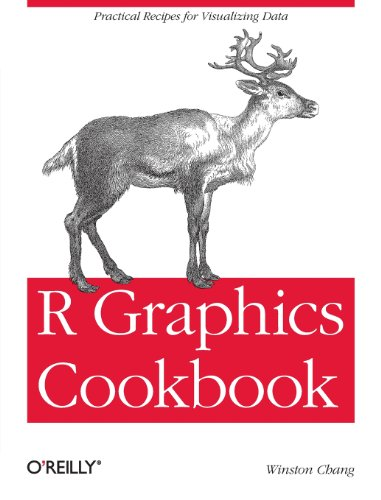
\includegraphics[scale=0.45]{rgraphicscookbook}
\end{column}

\begin{column}{0.5\textwidth}
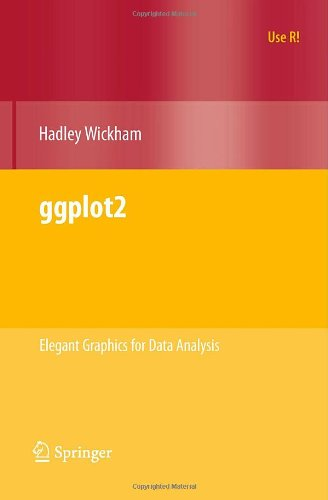
\includegraphics[scale=0.45]{ggplot2}
\end{column}
\end{columns}
\end{frame}

\begin{frame}{Online resources}
\begin{itemize}
\item ggplot2 official documentation:\\  \url{http://docs.ggplot2.org/current/}
\item R code related to ggplot2 cookbook:\\ \url{http://www.cookbook-r.com/Graphs/}
\item R code related to useR! ggplot2 book:\\ \url{http://ggplot2.org/book/}
\item Google groups to ask questions:\\ \url{ggplot2@googlegroups.com}
\item Statistical tools for high-throughput data analysis:\\ \url{http://www.sthda.com/english/wiki/ggplot2-essentials}
\item Github repository:\\ \url{https://github.com/yhat/ggplot/}
\item RStudio Cheat Sheet :\\ \url{http://www.rstudio.com/wp-content/uploads/2015/12/ggplot2-cheatsheet-2.0.pdf}
\end{itemize}
\end{frame}


\begin{frame}{Introduction}
\begin{itemize}
\item based on \textit{new} aesthetic principles
\item based on \textit{The grammar of graphics} developed by Wilkinson in 2005
\item efficient way to produce simple graphics with a length reduction of R code
\end{itemize}

\begin{alertblock}{Forget about R base graphics:}
\texttt{ plot(), hist(), par(), layout(), points(), lines(),legend()}
\end{alertblock}
\end{frame}

\begin{frame}{Principle}
ggplot2 is based on a \textbf{layer} system which can be used as objects.\\
\vspace{1cm}
Main layers
\begin{itemize}
\item data $\rightarrow$ raw data
\item mapping $\rightarrow$ graphic projection
\item geom $\rightarrow$ geometric objects (points, lines, polygons, ...)
\item stat $\rightarrow$ statistics transformation (histogram, model)
\item scale $\rightarrow$ aesthetics customization (colour, shape, size, axes, legend)
\item coord $\rightarrow$ coordinate system (axes, grid)
\item facet $\rightarrow$ subdivision (lattice, trellis)
\end{itemize}
\end{frame}

\begin{frame}{Base functions}
ggplot2 is based on two functions:
\vspace{0.5cm}
\begin{enumerate}
\item  \texttt{qplot()} for \textbf{q}uick \textbf{plot}
\begin{itemize}
\item easy and fast, but too simple in most cases
\item \texttt{qplot(x, y, data=data)}
\end{itemize}
\vspace{0.5cm}
\item \texttt{ggplot()}
\begin{itemize}
\item more complex but more powerful and flexible by adding \texttt{layers}
\item \texttt{ggplot(data=data, aes(x, y)) + layers}
\end{itemize}
\end{enumerate}
\end{frame}

%%%%%%%%%%%%%%%%%%%%%%%%%%%%%%%%%%%
\subsection{Data}

\begin{frame}[fragile]{Getting Started}

\begin{alertblock}{Data format}
Always work with a \texttt{data.frame}
\end{alertblock}

\vspace{1cm}

Our data frame is based on the Hecate Strait Synoptic Trawl Survey and simulated data.
\vspace{1cm}

Download all the codes from a Github repository:\newline \url{https://github.com/JBLecomte/ggplot2-Introduction.git}
\end{frame}

\begin{frame}[fragile]{Getting Started}
\begin{knitrout}\scriptsize
\definecolor{shadecolor}{rgb}{0.969, 0.969, 0.969}\color{fgcolor}\begin{kframe}
\begin{alltt}
\hlkwd{str}\hlstd{(df_data)}
\end{alltt}
\begin{verbatim}
## 'data.frame':	1909 obs. of  18 variables:
##  $ Year            : int  2005 2005 2005 2005 2005 2005 2005 2005 2005 2005 ...
##  $ Month           : int  7 7 7 7 7 7 7 7 7 7 ...
##  $ DURATION_MINUTES: int  21 20 21 21 20 20 20 21 21 20 ...
##  $ AREA            : Factor w/ 2 levels "5AB","5CD": 1 1 1 1 1 1 1 1 1 1 ...
##  $ Avg_net_depth   : num  -0.316 -0.435 -0.442 -0.234 -0.171 ...
##  $ Avg_net_temp    : num  0.3939 0.4339 0.3004 0.1335 -0.0267 ...
##  $ Date            : Date, format: "2005-07-06" "2005-07-06" ...
##  $ Lon             : num  -128 -128 -128 -128 -128 ...
##  $ Lat             : num  51.2 51.1 51.6 51.6 51.7 ...
##  $ X               : num  572025 570307 553665 551917 546338 ...
##  $ Y               : num  5668122 5665874 5717947 5719597 5723992 ...
##  $ X_km            : num  572 570 554 552 546 ...
##  $ Y_km            : num  5668 5666 5718 5720 5724 ...
##  $ Pres            : num  1 1 1 1 1 1 1 0 0 1 ...
##  $ Year_fac        : Factor w/ 5 levels "2005","2007",..: 1 1 1 1 1 1 1 1 1 1 ...
##  $ AREA_num        : num  1 1 1 1 1 1 1 1 1 1 ...
##  $ nFish           : int  1 1 2 3 1 1 1 0 1 0 ...
##  $ Biomass         : num  4.01 3.4 8.51 6.01 4.06 ...
\end{verbatim}
\end{kframe}
\end{knitrout}
\end{frame}

%%%%%%%%%%%%%%%%%%%%%%%
\subsection{Overview}
\begin{frame}[fragile]{A quick overview of the ggplot2 types}
\begin{itemize}
\item Points, as for a scatterplot: \lstinline{geom_point()}
\item Lines: \lstinline{geom_line()}
\item Histogram: \lstinline{geom_freqpoly(geom_histogram(), stat_bin())}
\item Boxplot: \lstinline{geom_boxplot()}
\item Polygon: \lstinline{geom_polygon()}
\item Draw rectangles: \lstinline{geom_raster()}
\item Smooth density estimate: \lstinline{geom_density()}
\item Ribbons and area plots: \lstinline{geom_ribbon(geom_area())}
\item Map: \lstinline{ggmap()}
\end{itemize}
\end{frame}

%%%%%%%%%%%%%%%%%%%%%%%%%%%%%%%%%%%
%% Example: scatter plot
\section{Scatter plot}
%%%%%%%%%%%%%%%%%%%%%%%%%%%%%%%%%%%

\begin{frame}[fragile]{Scatter plot: Depth and Biomass}
\begin{knitrout}\footnotesize
\definecolor{shadecolor}{rgb}{0.969, 0.969, 0.969}\color{fgcolor}\begin{kframe}
\begin{alltt}
\hlstd{sp} \hlkwb{<-} \hlkwd{ggplot}\hlstd{(}\hlkwc{data}\hlstd{=df_data,} \hlkwd{aes}\hlstd{(}\hlkwc{x}\hlstd{=Avg_net_depth,} \hlkwc{y}\hlstd{=Biomass))} \hlopt{+}
  \hlkwd{geom_point}\hlstd{(}\hlkwc{size}\hlstd{=}\hlnum{1}\hlstd{)}
\hlkwd{print}\hlstd{(sp)}
\end{alltt}
\end{kframe}

{\centering 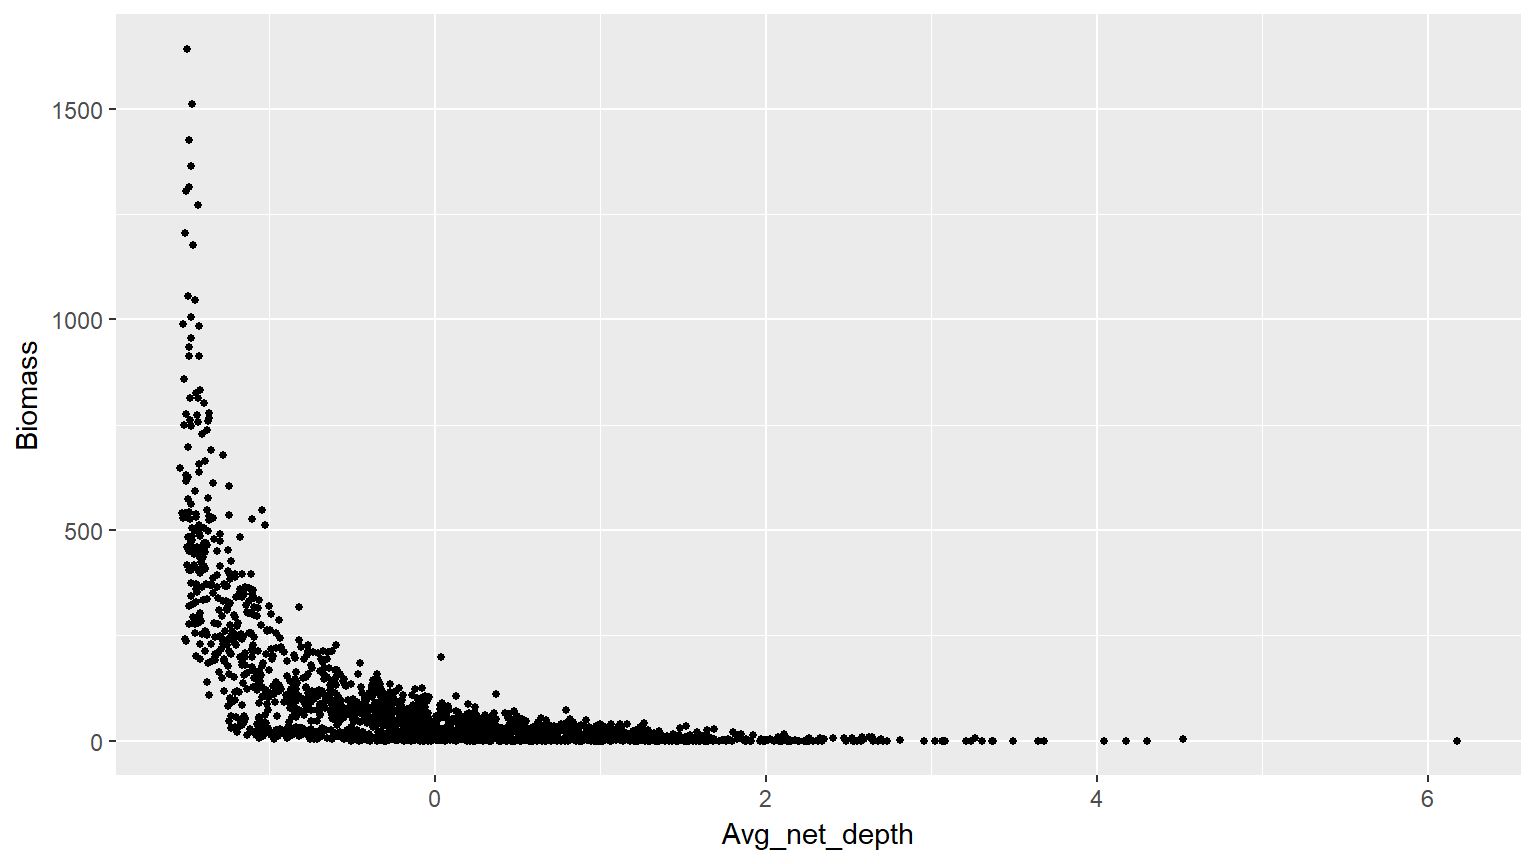
\includegraphics[width=.9\linewidth]{figure/sp_base-1} 

}



\end{knitrout}
\end{frame}

\begin{frame}[fragile]{Scatter plot with color: Depth and Biomass}
\begin{knitrout}\footnotesize
\definecolor{shadecolor}{rgb}{0.969, 0.969, 0.969}\color{fgcolor}\begin{kframe}
\begin{alltt}
\hlstd{sp_color} \hlkwb{<-} \hlkwd{ggplot}\hlstd{(df_data,} \hlkwd{aes}\hlstd{(}\hlkwc{x}\hlstd{=Avg_net_depth,} \hlkwc{y}\hlstd{=Biomass,}
                                \hlkwc{color}\hlstd{=AREA))} \hlopt{+}
  \hlkwd{geom_point}\hlstd{(}\hlkwc{size}\hlstd{=}\hlnum{1}\hlstd{)}
\hlkwd{print}\hlstd{(sp_color)}
\end{alltt}
\end{kframe}

{\centering 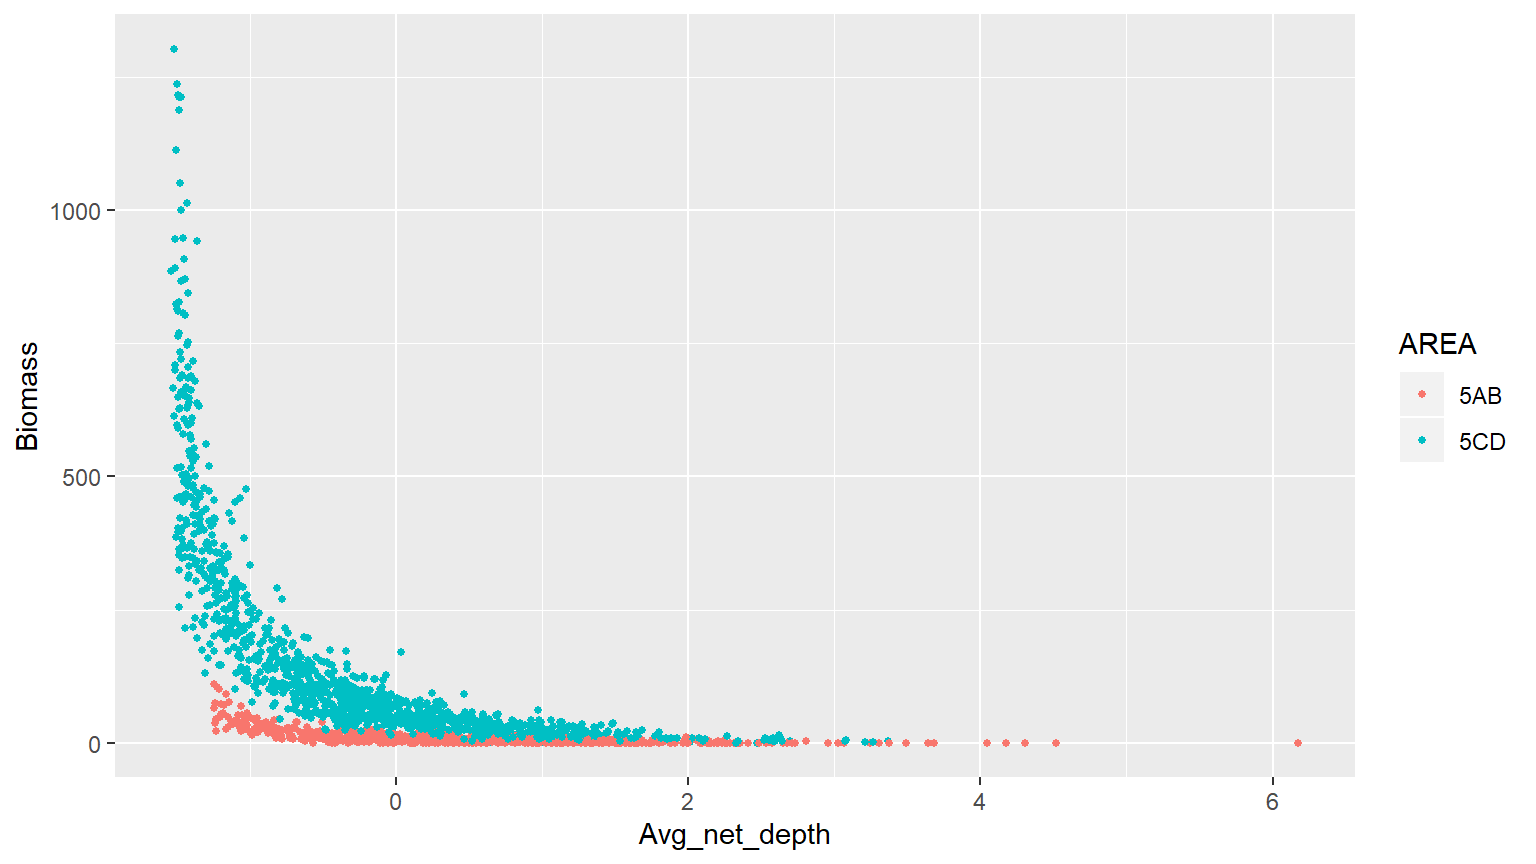
\includegraphics[width=.9\linewidth]{figure/sp_color-1} 

}



\end{knitrout}
\end{frame}


\begin{frame}[fragile]{Scatter plot with shape: Depth and Biomass}
\begin{knitrout}\footnotesize
\definecolor{shadecolor}{rgb}{0.969, 0.969, 0.969}\color{fgcolor}\begin{kframe}
\begin{alltt}
\hlstd{sp_shape} \hlkwb{<-} \hlkwd{ggplot}\hlstd{(df_data,} \hlkwd{aes}\hlstd{(}\hlkwc{x}\hlstd{=Avg_net_depth,} \hlkwc{y}\hlstd{=Biomass,}
                                \hlkwc{color}\hlstd{=AREA,} \hlkwc{shape}\hlstd{=Year_fac))} \hlopt{+}
  \hlkwd{geom_point}\hlstd{(}\hlkwc{size}\hlstd{=}\hlnum{1}\hlstd{)}
\hlkwd{print}\hlstd{(sp_shape)}
\end{alltt}
\end{kframe}

{\centering 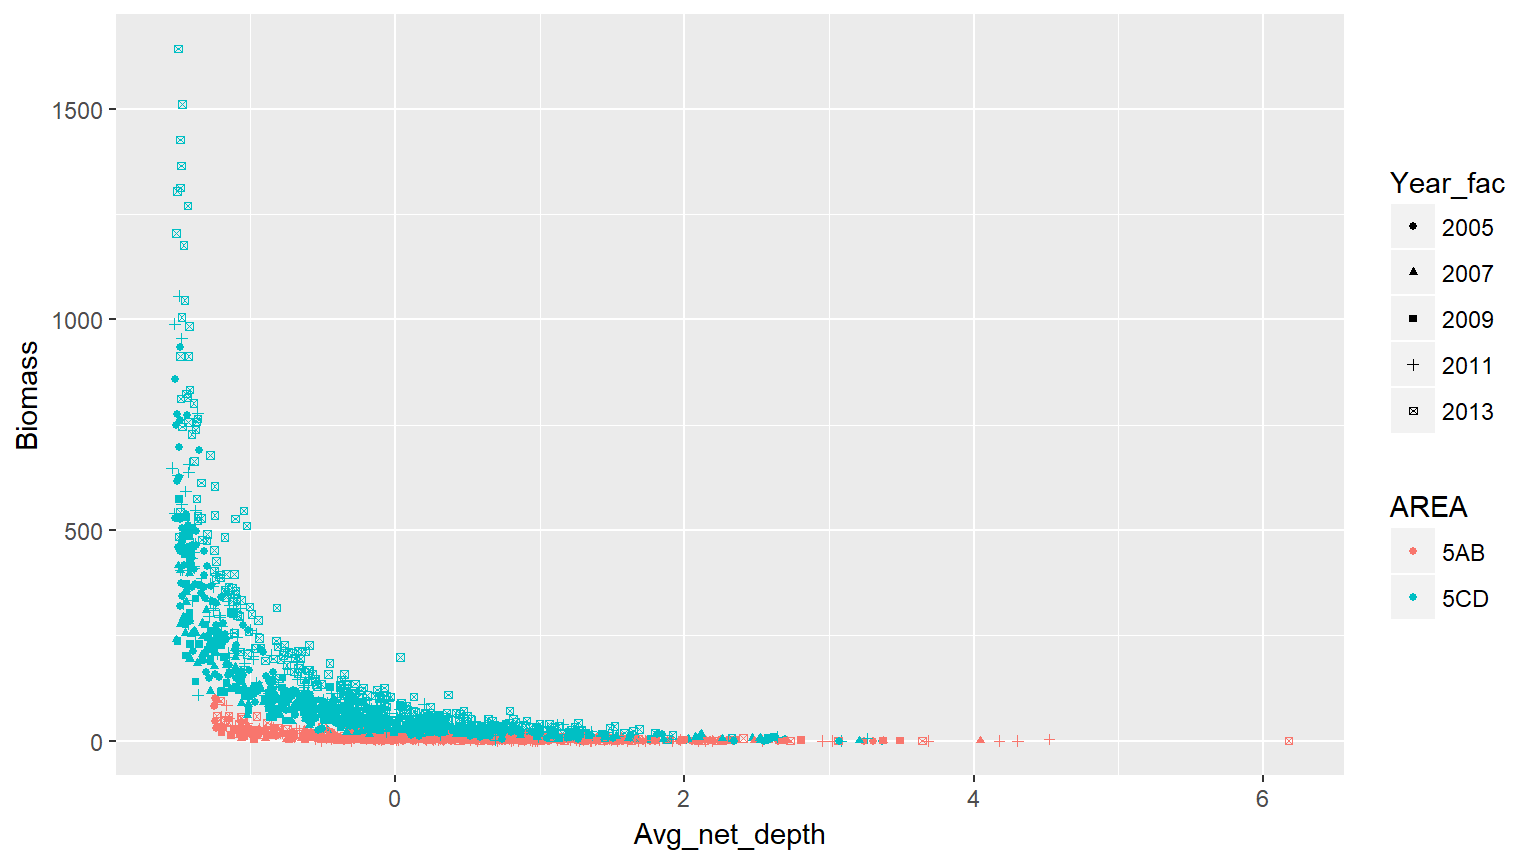
\includegraphics[width=.9\linewidth]{figure/sp_shape-1} 

}



\end{knitrout}
\end{frame}

\begin{frame}[fragile]{Scatter plot with continuous color: Depth and Biomass}
\begin{knitrout}\footnotesize
\definecolor{shadecolor}{rgb}{0.969, 0.969, 0.969}\color{fgcolor}\begin{kframe}
\begin{alltt}
\hlstd{sp_color_cont} \hlkwb{<-} \hlkwd{ggplot}\hlstd{(df_data,} \hlkwd{aes}\hlstd{(}\hlkwc{x}\hlstd{=Avg_net_depth,} \hlkwc{y}\hlstd{=Biomass,}
                                     \hlkwc{color}\hlstd{=Avg_net_temp))} \hlopt{+}
  \hlkwd{geom_point}\hlstd{(}\hlkwc{size}\hlstd{=}\hlnum{1}\hlstd{)}
\hlkwd{print}\hlstd{(sp_color_cont)}
\end{alltt}
\end{kframe}

{\centering 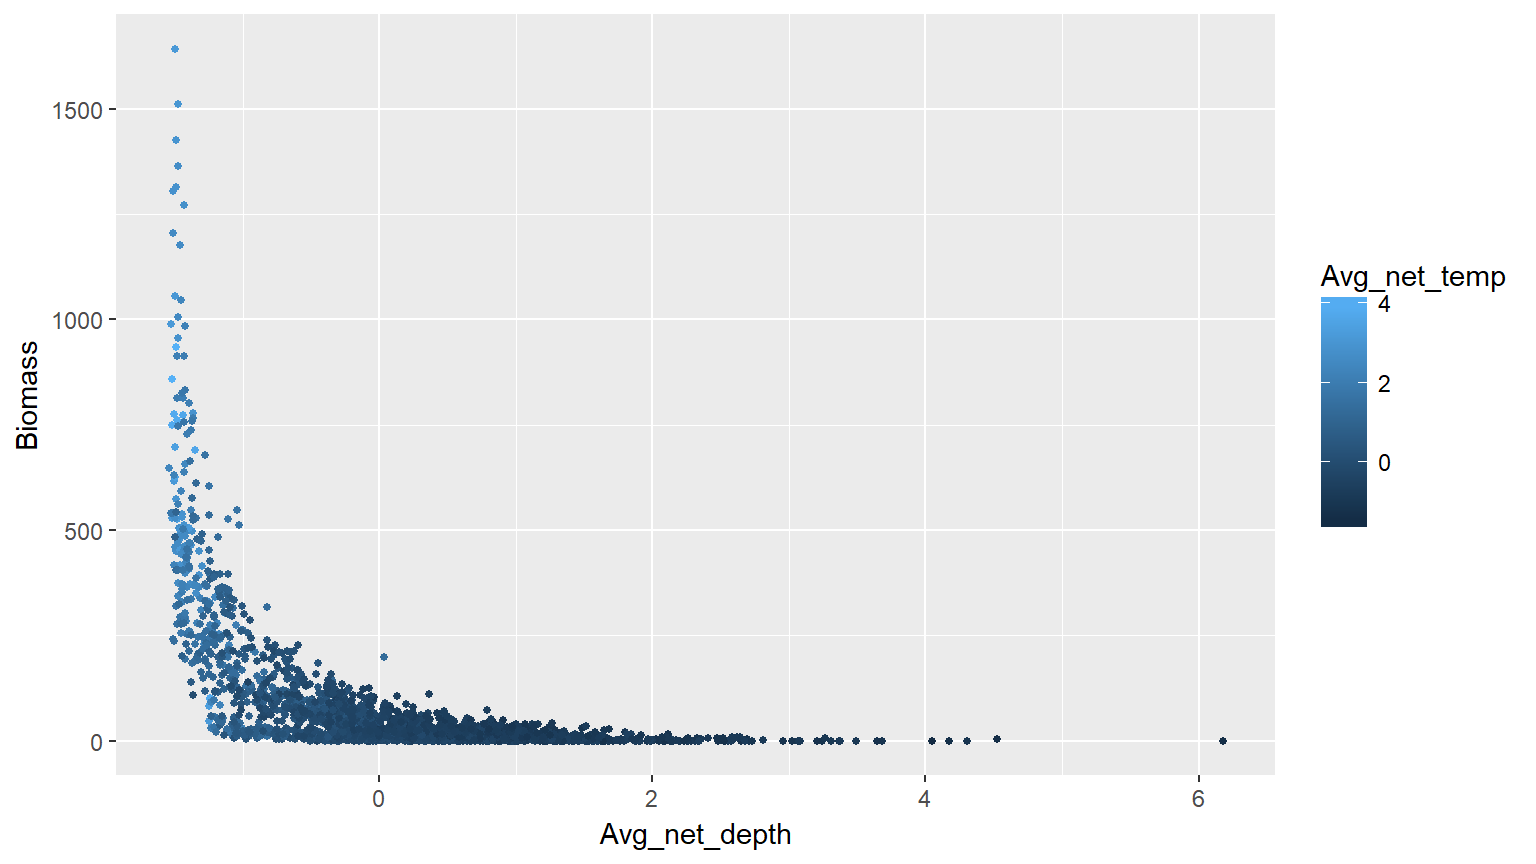
\includegraphics[width=.9\linewidth]{figure/sp_color_cont-1} 

}



\end{knitrout}
\end{frame}


\begin{frame}[fragile]{Scatter plot with size: Depth and Biomass}
\begin{knitrout}\footnotesize
\definecolor{shadecolor}{rgb}{0.969, 0.969, 0.969}\color{fgcolor}\begin{kframe}
\begin{alltt}
\hlstd{sp_area} \hlkwb{<-} \hlkwd{ggplot}\hlstd{(df_data,} \hlkwd{aes}\hlstd{(}\hlkwc{x}\hlstd{=Avg_net_depth,} \hlkwc{y}\hlstd{=Biomass,}
                               \hlkwc{size}\hlstd{=nFish))} \hlopt{+}
  \hlkwd{geom_point}\hlstd{(}\hlkwc{shape}\hlstd{=}\hlnum{17}\hlstd{)}
\hlkwd{print}\hlstd{(sp_area)}
\end{alltt}
\end{kframe}

{\centering 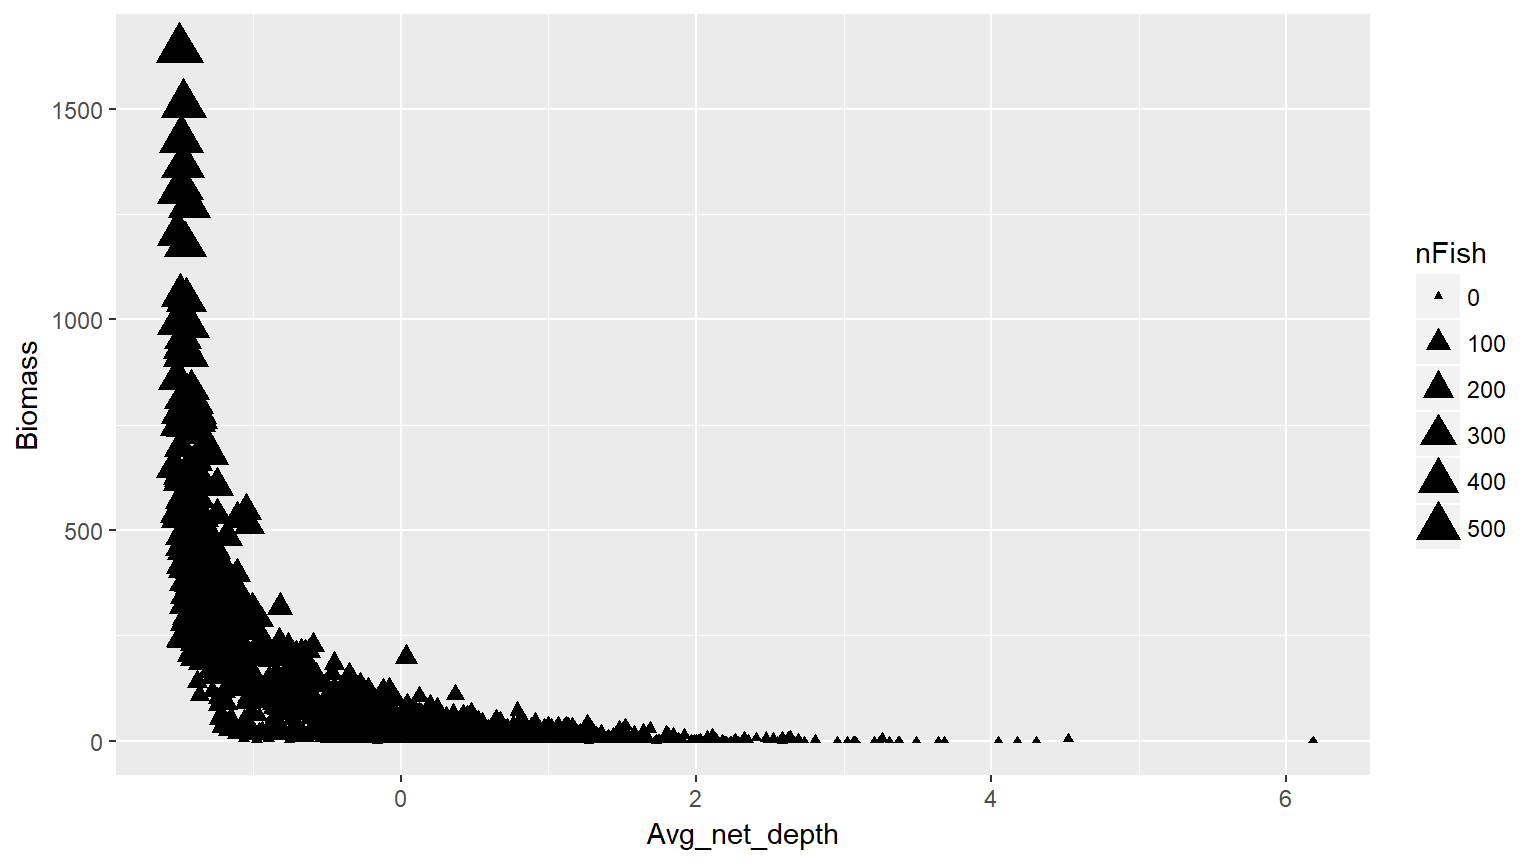
\includegraphics[width=.9\linewidth]{figure/sp_color_size-1} 

}



\end{knitrout}
\end{frame}

\begin{frame}[fragile]{Improvement of a plot}
\begin{knitrout}\footnotesize
\definecolor{shadecolor}{rgb}{0.969, 0.969, 0.969}\color{fgcolor}\begin{kframe}
\begin{alltt}
\hlstd{sp_shape} \hlkwb{<-} \hlkwd{ggplot}\hlstd{(df_data,} \hlkwd{aes}\hlstd{(}\hlkwc{x}\hlstd{=Avg_net_depth,} \hlkwc{y}\hlstd{=Biomass,}
                                \hlkwc{color}\hlstd{=AREA,} \hlkwc{shape}\hlstd{=Year_fac))} \hlopt{+}
  \hlkwd{geom_point}\hlstd{(}\hlkwc{size}\hlstd{=}\hlnum{1}\hlstd{)}
\hlkwd{print}\hlstd{(sp_shape)}
\end{alltt}
\end{kframe}

{\centering 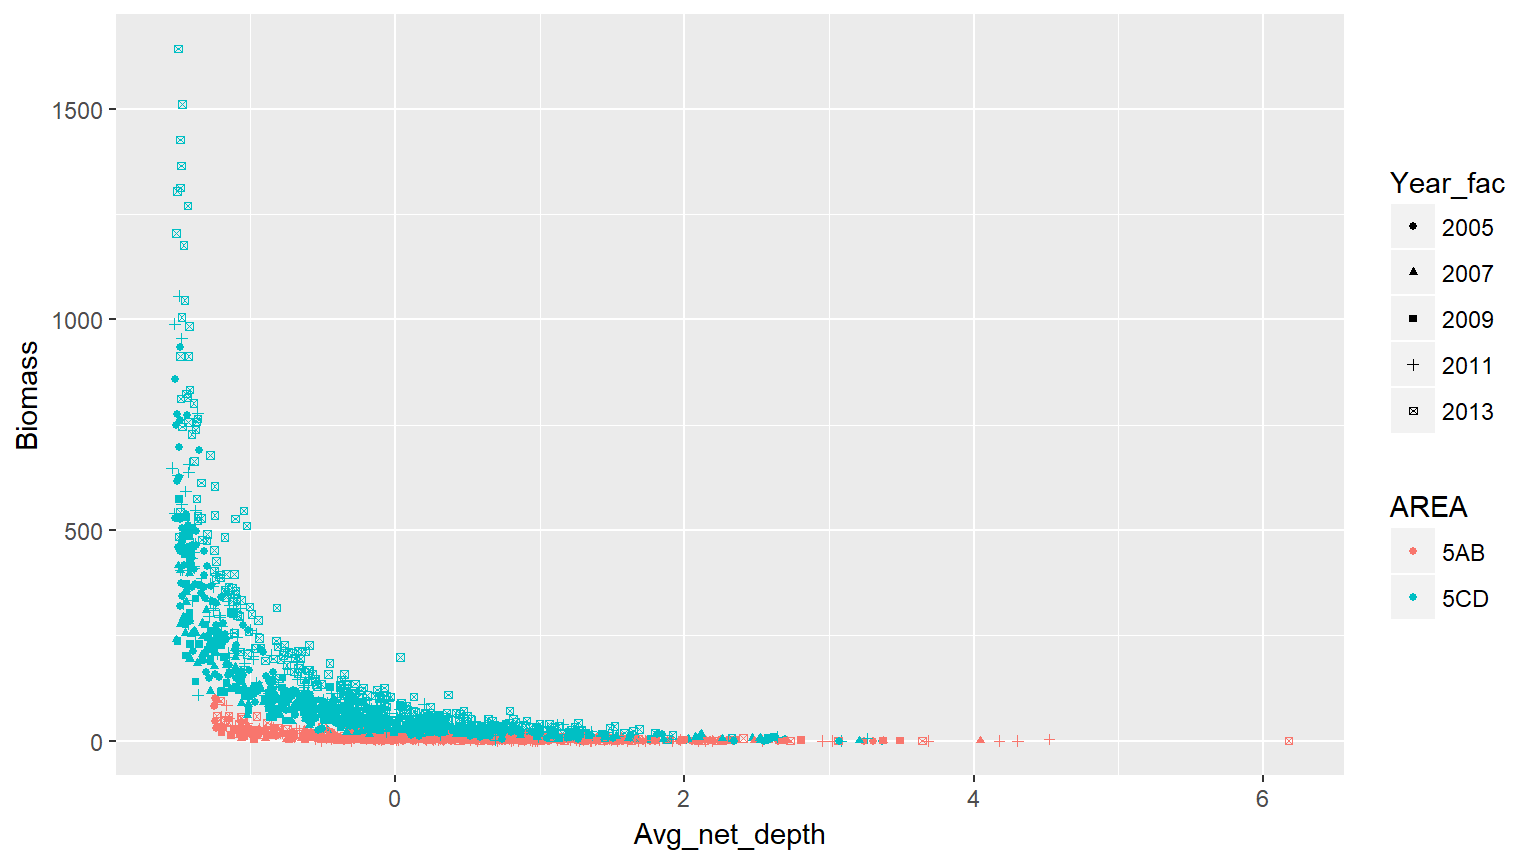
\includegraphics[width=.9\linewidth]{figure/sp_shape2-1} 

}



\end{knitrout}
\end{frame}

\begin{frame}[fragile]{Improvement of a plot: axes names}
\begin{knitrout}\footnotesize
\definecolor{shadecolor}{rgb}{0.969, 0.969, 0.969}\color{fgcolor}\begin{kframe}
\begin{alltt}
\hlstd{sp_shape_imp1} \hlkwb{<-} \hlstd{sp_shape} \hlopt{+}
  \hlkwd{xlab}\hlstd{(}\hlstr{'Average net depth (m)'}\hlstd{)} \hlopt{+}
  \hlkwd{ylab}\hlstd{(}\hlstr{'Biomass (kg)'}\hlstd{)}
\hlkwd{print}\hlstd{(sp_shape_imp1)}
\end{alltt}
\end{kframe}

{\centering 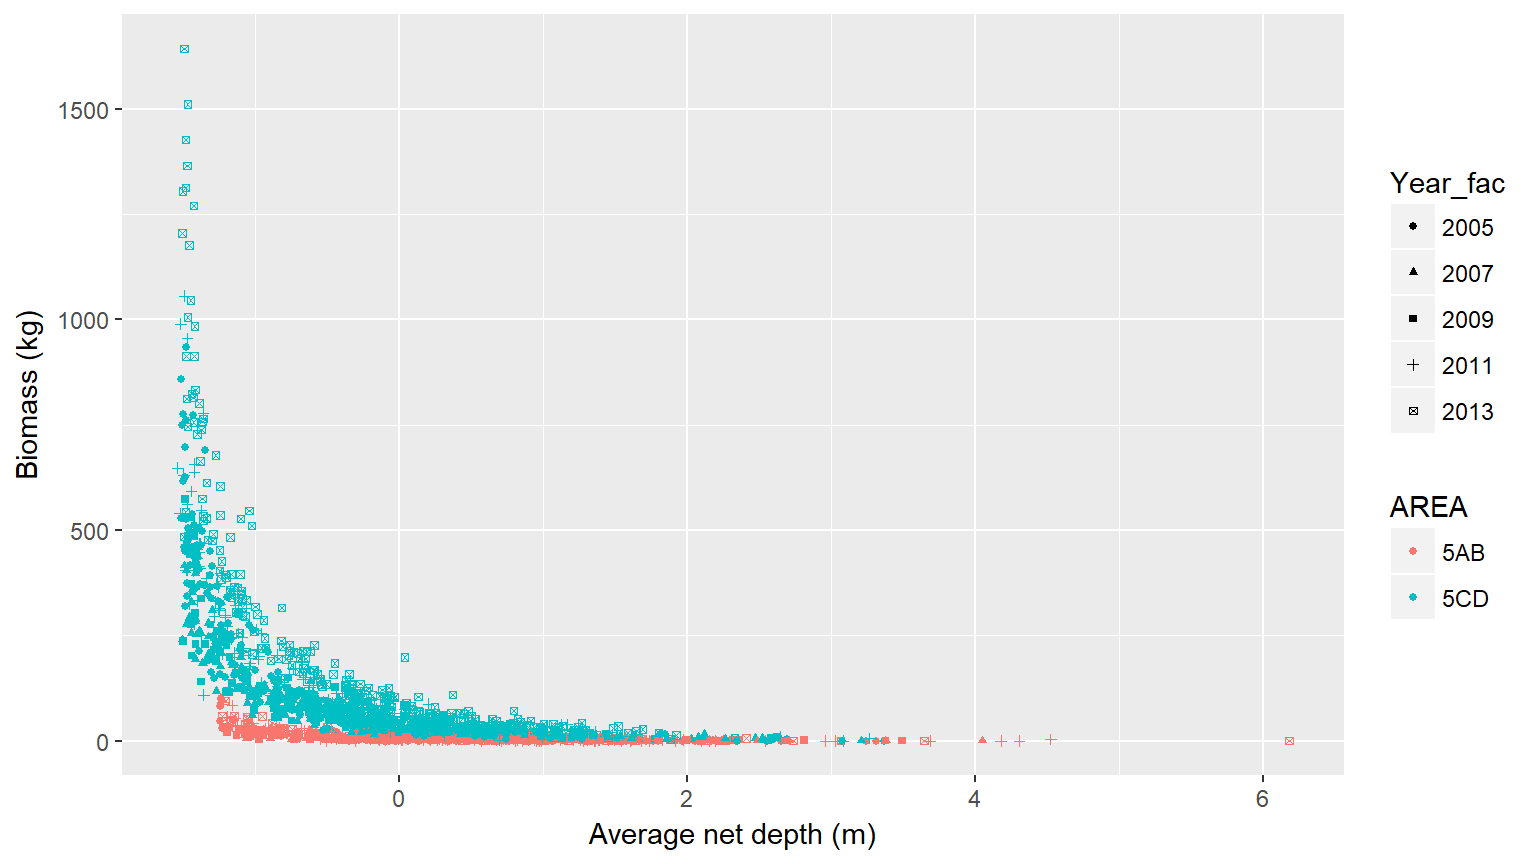
\includegraphics[width=.9\linewidth]{figure/sp_shape_imp1-1} 

}



\end{knitrout}
\end{frame}

\begin{frame}[fragile]{Improvement of a plot: axes options}
\begin{knitrout}\footnotesize
\definecolor{shadecolor}{rgb}{0.969, 0.969, 0.969}\color{fgcolor}\begin{kframe}
\begin{alltt}
\hlkwd{scale_x_continuous}\hlstd{(name, breaks, labels, limits, trans)}
\hlkwd{scale_y_continuous}\hlstd{(name, breaks, labels, limits, trans)}
\end{alltt}
\end{kframe}
\end{knitrout}
\begin{itemize}

\item    name : x or y axis labels
\item    breaks : to control the breaks in the guide (axis ticks, grid lines,...).
Among the possible values, there are :
NULL : hide all breaks
waiver() : the default break computation a character or numeric vector specifying the breaks to display
\item labels : labels of axis tick marks. Allowed values are :
NULL for no labels
waiver() for the default labels
character vector to be used for break labels
\item limits : a numeric vector specifying x or y axis limits (min, max)
\item trans for axis transformations. Possible values are "log2", "log10"
\end{itemize}
\end{frame}

\begin{frame}[fragile]{Improvement of a plot: axes options}
\begin{knitrout}\footnotesize
\definecolor{shadecolor}{rgb}{0.969, 0.969, 0.969}\color{fgcolor}\begin{kframe}
\begin{alltt}
\hlstd{sp_shape_imp1} \hlkwb{<-} \hlstd{sp_shape_imp1} \hlopt{+}
  \hlkwd{scale_x_continuous}\hlstd{(}\hlkwc{name}\hlstd{=}\hlstr{'Average net depth (m)'}\hlstd{,}
                     \hlkwc{breaks}\hlstd{=}\hlkwd{seq}\hlstd{(}\hlopt{-}\hlnum{4}\hlstd{,}\hlnum{7}\hlstd{,}\hlnum{2}\hlstd{),} \hlkwc{limits}\hlstd{=}\hlkwd{c}\hlstd{(}\hlopt{-}\hlnum{4}\hlstd{,}\hlnum{7}\hlstd{))}
\hlkwd{print}\hlstd{(sp_shape_imp1)}
\end{alltt}
\end{kframe}

{\centering 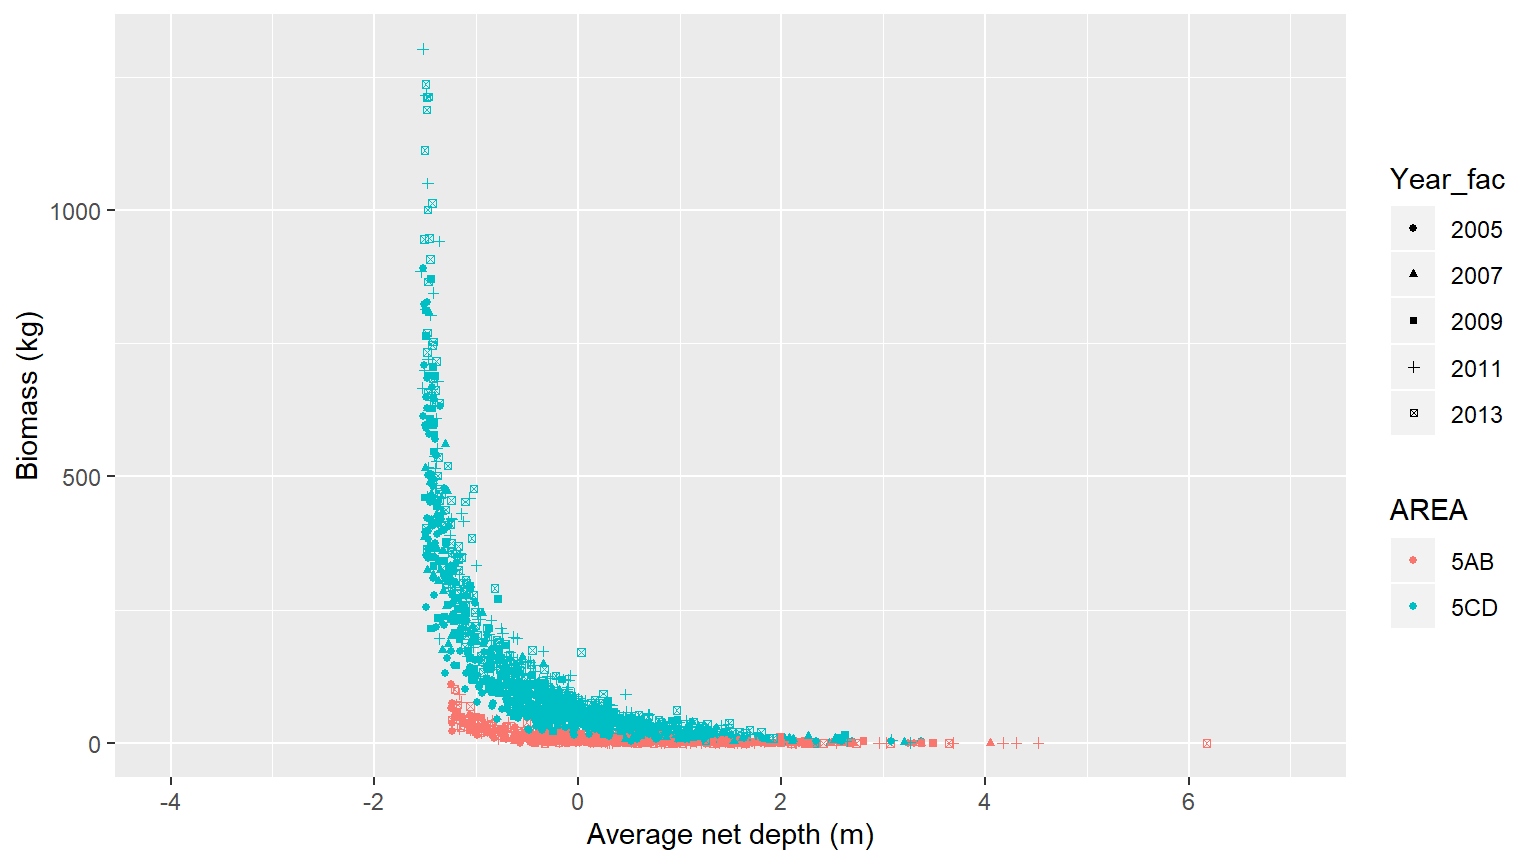
\includegraphics[width=.9\linewidth]{figure/sp_shape_imp1x-1} 

}



\end{knitrout}
\end{frame}

\begin{frame}[fragile]{Improvement of a plot: legend titles}
\begin{knitrout}\footnotesize
\definecolor{shadecolor}{rgb}{0.969, 0.969, 0.969}\color{fgcolor}\begin{kframe}
\begin{alltt}
\hlstd{sp_shape_imp2} \hlkwb{<-} \hlkwd{ggplot}\hlstd{(df_data,} \hlkwd{aes}\hlstd{(}\hlkwc{x}\hlstd{=Avg_net_depth,} \hlkwc{y}\hlstd{=Biomass,}
                                     \hlkwc{color}\hlstd{=AREA,} \hlkwc{shape}\hlstd{=Year_fac))} \hlopt{+}
  \hlkwd{geom_point}\hlstd{(}\hlkwc{size}\hlstd{=}\hlnum{1}\hlstd{)} \hlopt{+} \hlkwd{xlab}\hlstd{(}\hlstr{'Average net depth (m)'}\hlstd{)} \hlopt{+}
  \hlkwd{scale_shape_discrete}\hlstd{(}\hlkwc{name}\hlstd{=}\hlstr{"Years"}\hlstd{)} \hlopt{+} \hlkwd{scale_color_discrete}\hlstd{(}\hlkwc{name}\hlstd{=}\hlstr{"Area"}\hlstd{)}
\hlkwd{print}\hlstd{(sp_shape_imp2)}
\end{alltt}
\end{kframe}

{\centering 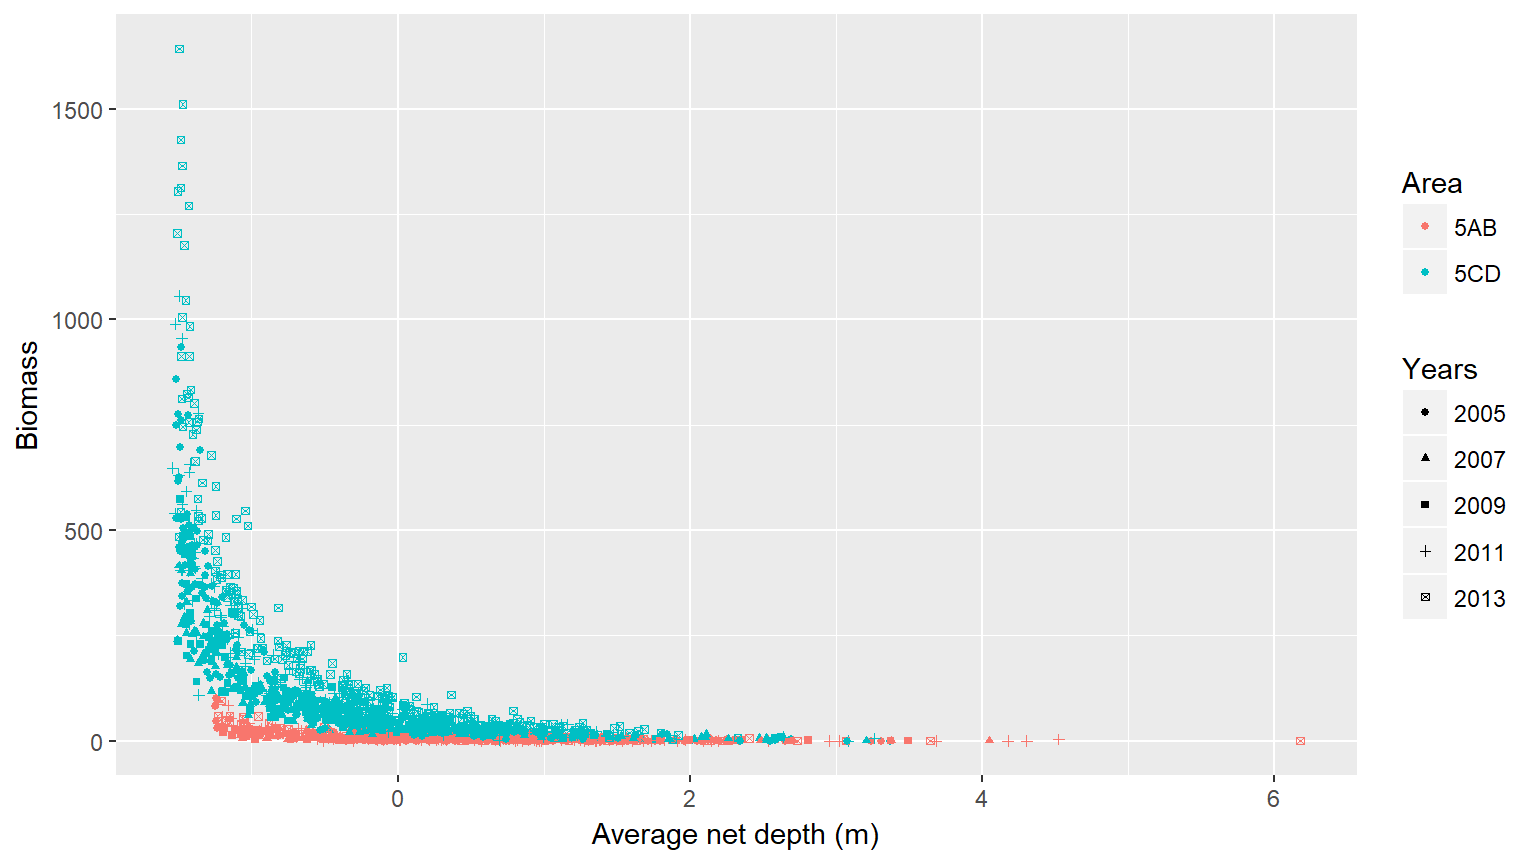
\includegraphics[width=.9\linewidth]{figure/sp_shape_imp2-1} 

}



\end{knitrout}
\end{frame}


\begin{frame}[fragile]{Improvement of a plot: plot title}
\begin{knitrout}\footnotesize
\definecolor{shadecolor}{rgb}{0.969, 0.969, 0.969}\color{fgcolor}\begin{kframe}
\begin{alltt}
\hlstd{sp_shape_imp3} \hlkwb{<-} \hlstd{sp_shape_imp2} \hlopt{+}
  \hlkwd{ggtitle}\hlstd{(}\hlstr{"Biomass of species X and average net depth"}\hlstd{)}
\hlkwd{print}\hlstd{(sp_shape_imp3)}
\end{alltt}
\end{kframe}

{\centering 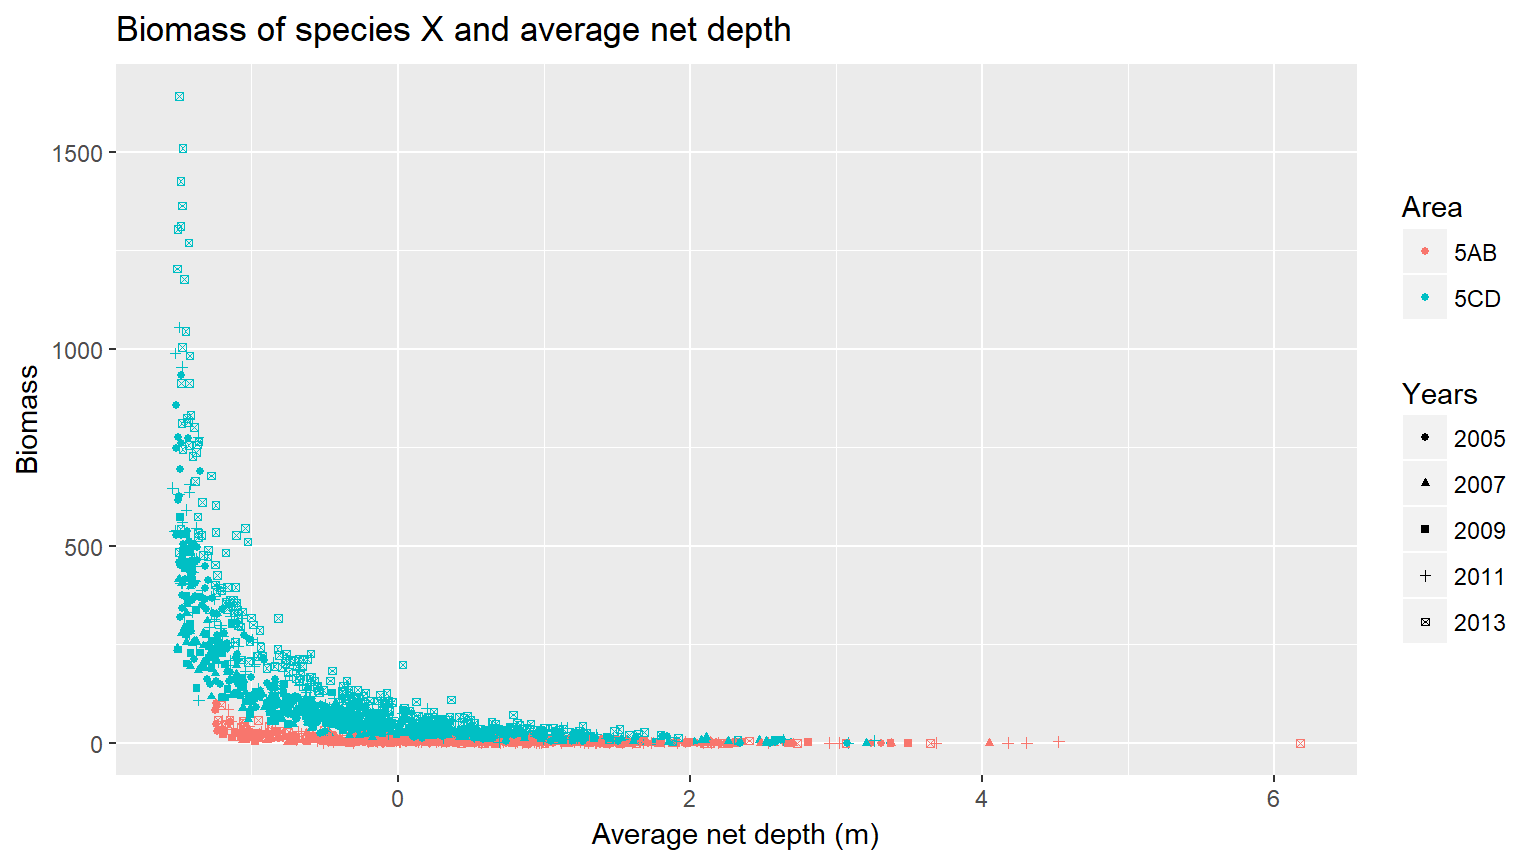
\includegraphics[width=.9\linewidth]{figure/sp_shape_imp3-1} 

}



\end{knitrout}
\end{frame}

%%%%%%%%%%%%%%%%%%%%%%%%%%%%%%%%%%%%%%%%%%%%%%%%%%%%%%%%%%%%%%%%%%%%%%%%%%%%%%%%
%% Example: scatter plot with discrete color
\section{Colors}
%%%%%%%%%%%%%%%%%%%%%%%%%%%%%%%%%%%%%%%%%%%%%%%%%%%%%%%%%%%%%%%%%%%%%%%%%%%%%%%%

%%%%%%%%%%%%%%%%%%%%%%%
\subsection{Colors for discrete variables}

\begin{frame}[fragile]{Discrete color scale}
\begin{knitrout}\footnotesize
\definecolor{shadecolor}{rgb}{0.969, 0.969, 0.969}\color{fgcolor}\begin{kframe}
\begin{alltt}
\hlstd{sp_c} \hlkwb{<-} \hlkwd{ggplot}\hlstd{(df_data,} \hlkwd{aes}\hlstd{(}\hlkwc{x}\hlstd{=Avg_net_depth,} \hlkwc{y}\hlstd{=Biomass,}
                            \hlkwc{color}\hlstd{=Year_fac))} \hlopt{+}
  \hlkwd{geom_point}\hlstd{(}\hlkwc{alpha}\hlstd{=}\hlnum{0.8}\hlstd{,} \hlkwc{size}\hlstd{=}\hlnum{1}\hlstd{)} \hlopt{+} \hlkwd{xlab}\hlstd{(}\hlstr{'Average net depth (m)'}\hlstd{)}
\hlkwd{print}\hlstd{(sp_c)}
\end{alltt}
\end{kframe}

{\centering 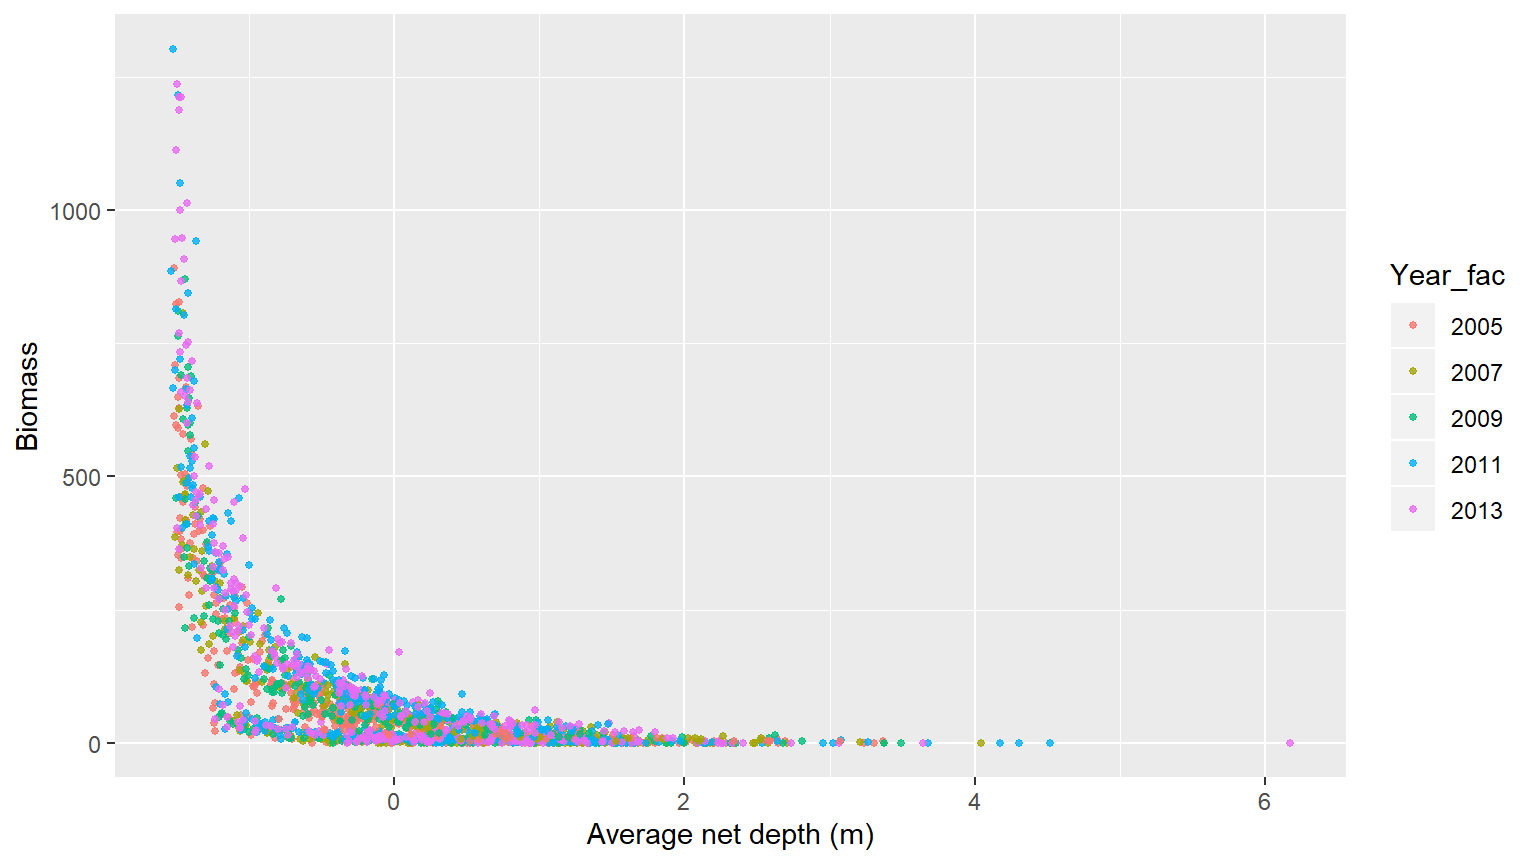
\includegraphics[width=.9\linewidth]{figure/sp_discrete_color1-1} 

}



\end{knitrout}
\end{frame}

%%%%%%%%%%%%%%%%%%%%%%%
\subsubsection{\lstinline{scale_colour_hue}}

\begin{frame}[fragile]{Discrete color scale: \lstinline{scale_colour_hue}}
\begin{knitrout}\footnotesize
\definecolor{shadecolor}{rgb}{0.969, 0.969, 0.969}\color{fgcolor}\begin{kframe}
\begin{alltt}
\hlcom{# Adjust luminosity and chroma}
\hlstd{sp_c_hue} \hlkwb{<-} \hlstd{sp_c} \hlopt{+}
  \hlkwd{scale_colour_hue}\hlstd{(}\hlkwc{name}\hlstd{=}\hlstr{'Year'}\hlstd{,} \hlkwc{l}\hlstd{=}\hlnum{70}\hlstd{,} \hlkwc{c}\hlstd{=}\hlnum{150}\hlstd{)}
\hlkwd{print}\hlstd{(sp_c_hue)}
\end{alltt}
\end{kframe}

{\centering 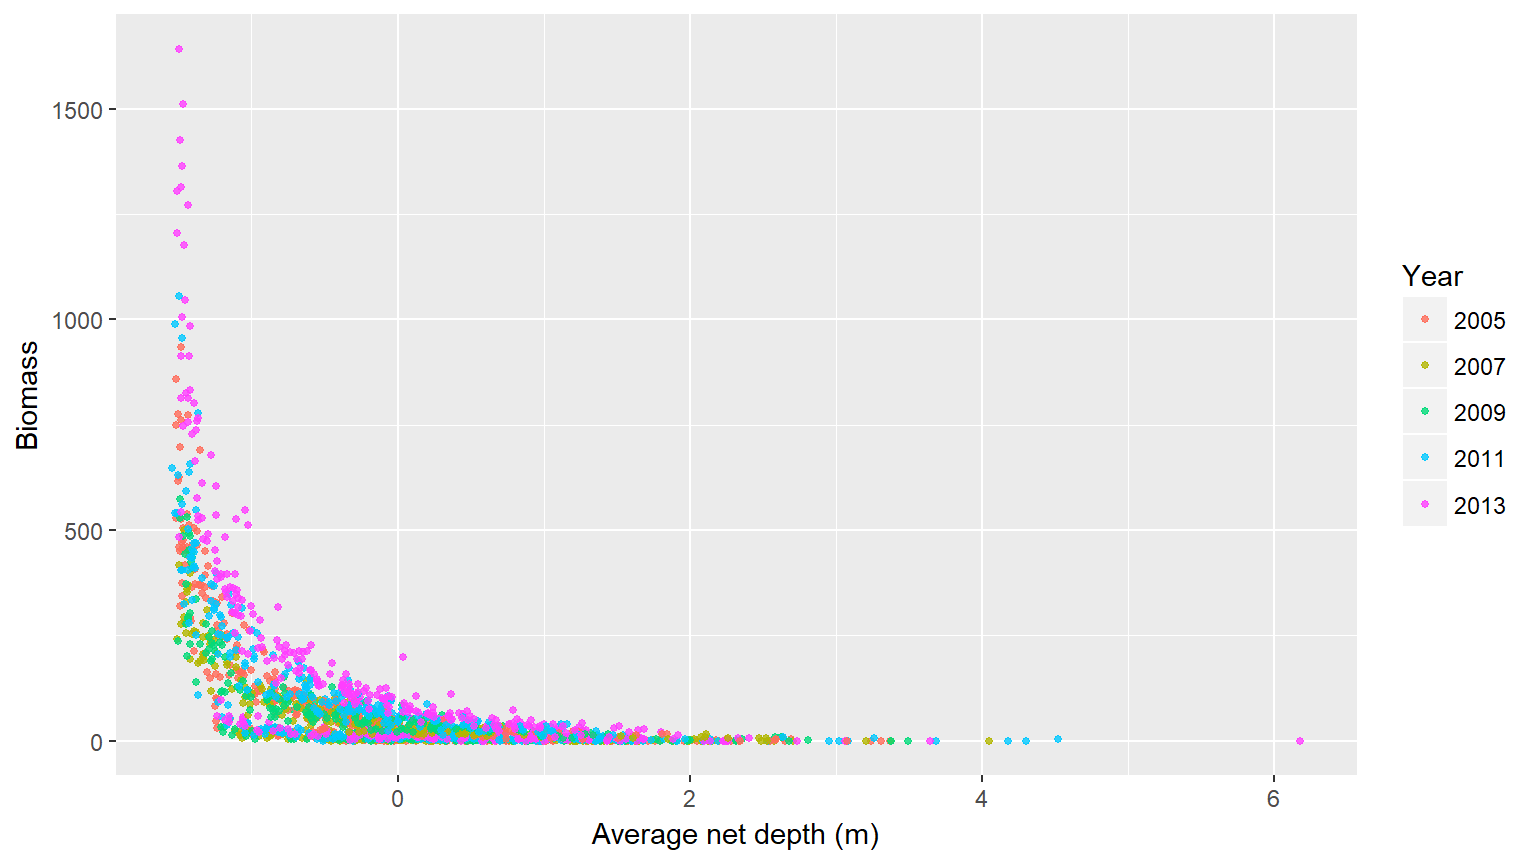
\includegraphics[width=.9\linewidth]{figure/sp_discrete_color_hue1-1} 

}



\end{knitrout}
\end{frame}

\begin{frame}[fragile]{Discrete color scale: \lstinline{scale_colour_hue}}
\begin{knitrout}\footnotesize
\definecolor{shadecolor}{rgb}{0.969, 0.969, 0.969}\color{fgcolor}\begin{kframe}
\begin{alltt}
\hlcom{# Adjust luminosity and chroma}
\hlstd{sp_c_hue} \hlkwb{<-} \hlstd{sp_c} \hlopt{+}
  \hlkwd{scale_colour_hue}\hlstd{(}\hlkwc{name}\hlstd{=}\hlstr{'Year'}\hlstd{,} \hlkwc{l}\hlstd{=}\hlnum{10}\hlstd{,} \hlkwc{c}\hlstd{=}\hlnum{150}\hlstd{)}
\hlkwd{print}\hlstd{(sp_c_hue)}
\end{alltt}
\end{kframe}

{\centering 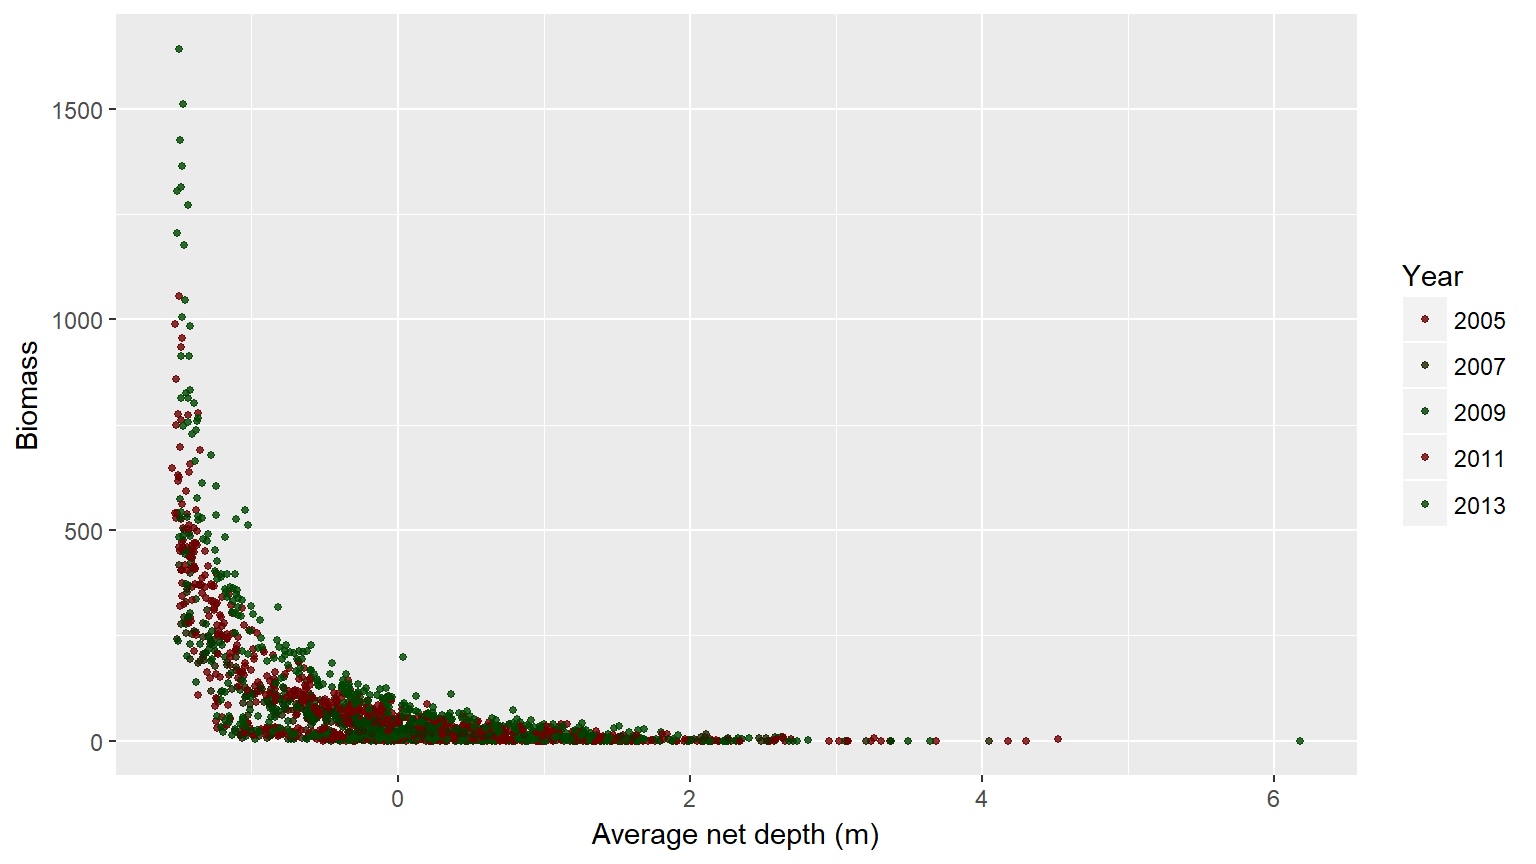
\includegraphics[width=.9\linewidth]{figure/sp_discrete_color_hue2-1} 

}



\end{knitrout}
\end{frame}

\begin{frame}[fragile]{Discrete color scale: \lstinline{scale_colour_hue}}
\begin{knitrout}\footnotesize
\definecolor{shadecolor}{rgb}{0.969, 0.969, 0.969}\color{fgcolor}\begin{kframe}
\begin{alltt}
\hlcom{# Adjust luminosity and chroma}
\hlstd{sp_c_hue} \hlkwb{<-} \hlstd{sp_c} \hlopt{+}
  \hlkwd{scale_colour_hue}\hlstd{(}\hlkwc{name}\hlstd{=}\hlstr{'Year'}\hlstd{,} \hlkwc{l}\hlstd{=}\hlnum{70}\hlstd{,} \hlkwc{c}\hlstd{=}\hlnum{50}\hlstd{)}
\hlkwd{print}\hlstd{(sp_c_hue)}
\end{alltt}
\end{kframe}

{\centering 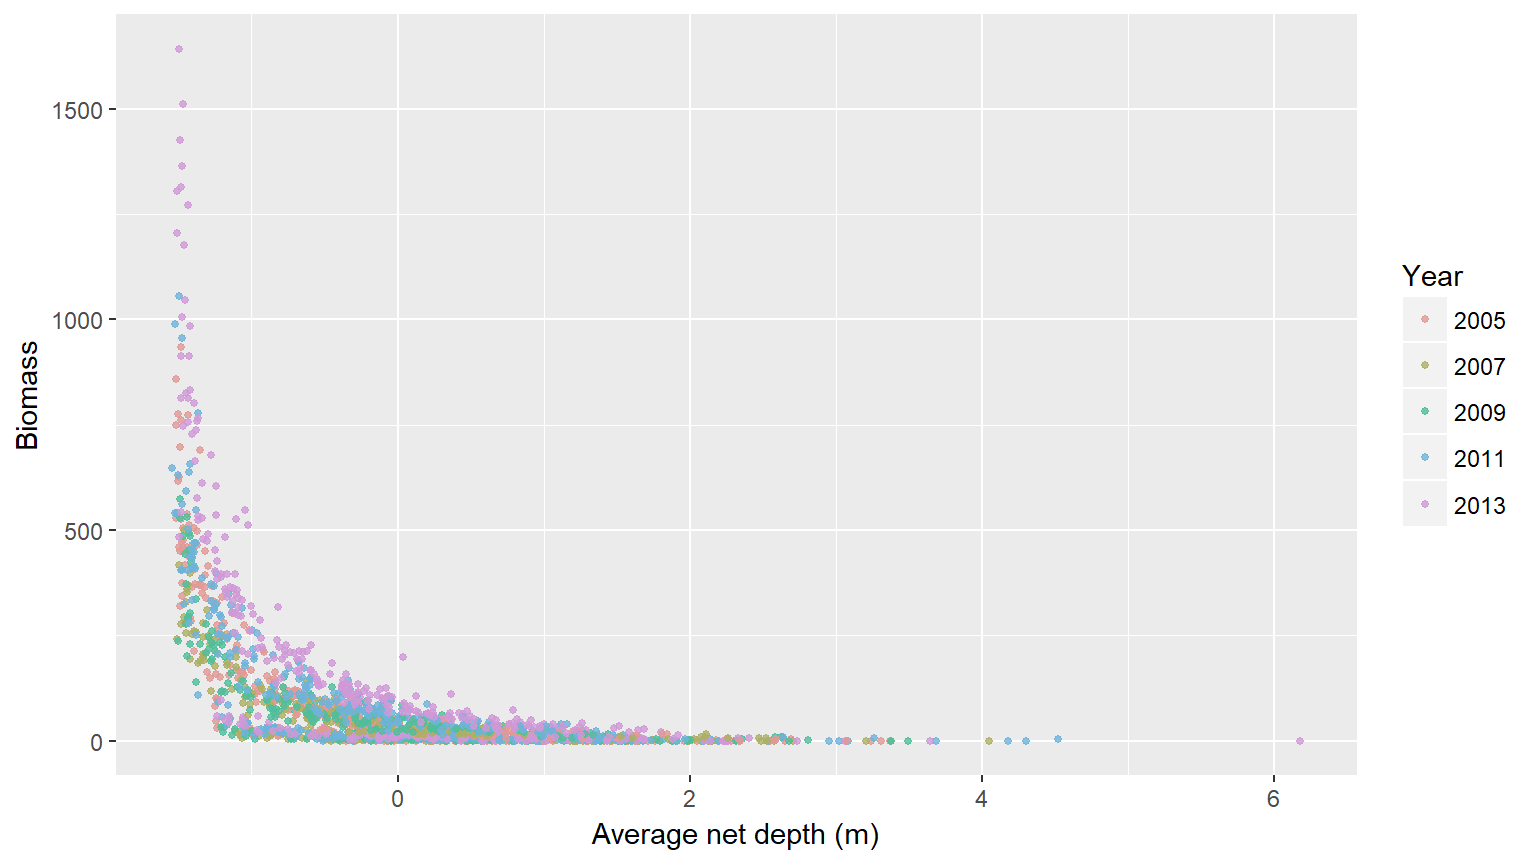
\includegraphics[width=.9\linewidth]{figure/sp_discrete_color_hue2b-1} 

}



\end{knitrout}
\end{frame}

\begin{frame}[fragile]{Discrete color scale: \lstinline{scale_colour_hue}}
\begin{knitrout}\footnotesize
\definecolor{shadecolor}{rgb}{0.969, 0.969, 0.969}\color{fgcolor}\begin{kframe}
\begin{alltt}
\hlcom{# Change range of hues used}
\hlstd{sp_c_hue} \hlkwb{<-} \hlstd{sp_c} \hlopt{+}
  \hlkwd{scale_colour_hue}\hlstd{(}\hlkwc{name}\hlstd{=}\hlstr{'Year'}\hlstd{,} \hlkwc{h}\hlstd{=}\hlkwd{c}\hlstd{(}\hlnum{0}\hlstd{,} \hlnum{90}\hlstd{))}
\hlkwd{print}\hlstd{(sp_c_hue)}
\end{alltt}
\end{kframe}

{\centering 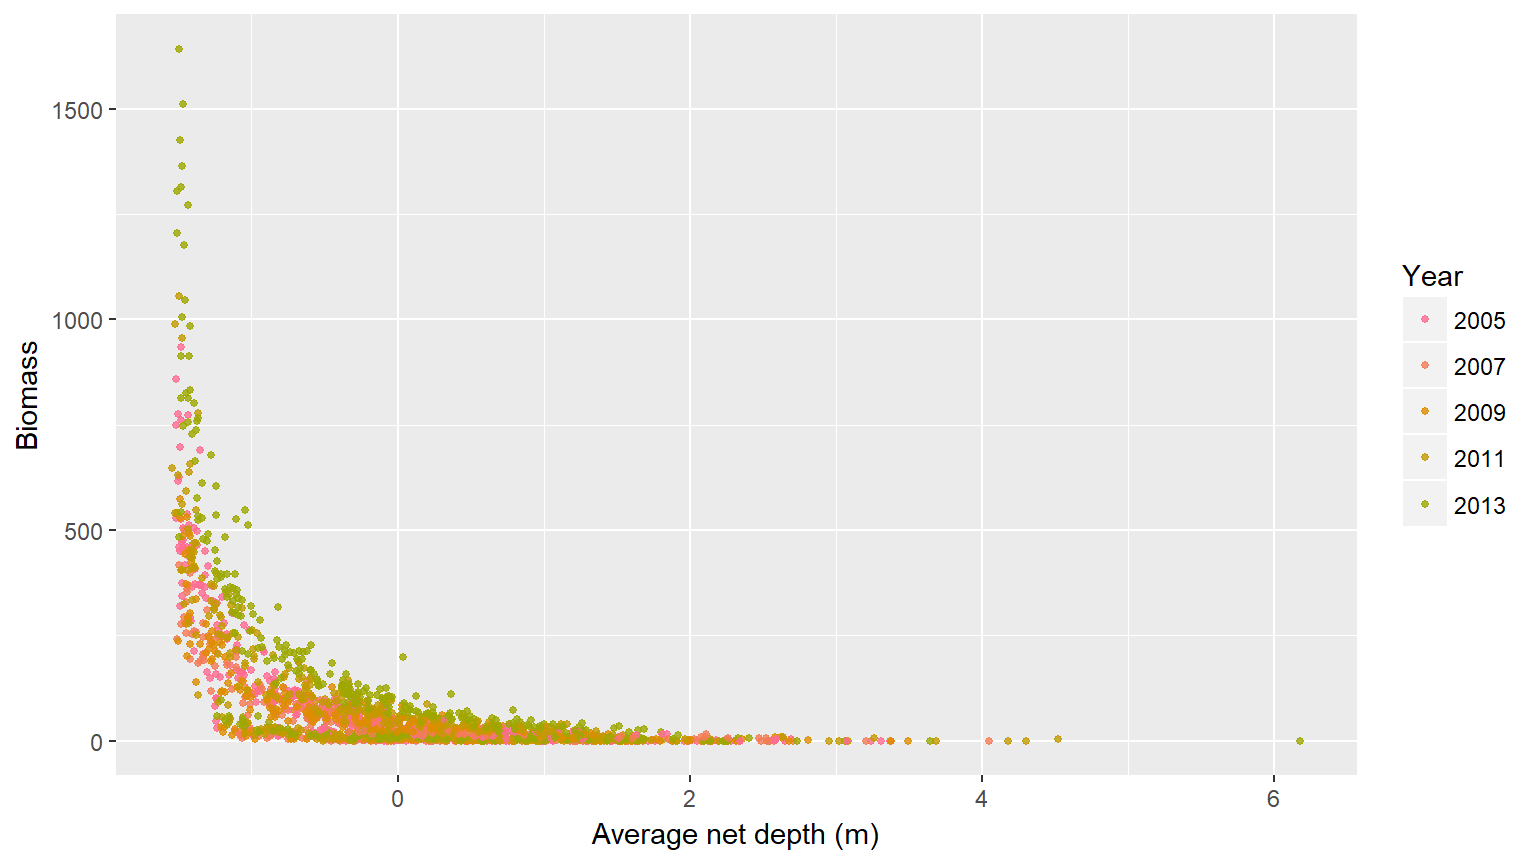
\includegraphics[width=.9\linewidth]{figure/sp_discrete_color_hue3-1} 

}



\end{knitrout}
\end{frame}

\begin{frame}[fragile]{Discrete color scale: \lstinline{scale_colour_hue}}
\begin{knitrout}\footnotesize
\definecolor{shadecolor}{rgb}{0.969, 0.969, 0.969}\color{fgcolor}\begin{kframe}
\begin{alltt}
\hlcom{# Change range of hues used}
\hlstd{sp_c_hue} \hlkwb{<-} \hlstd{sp_c} \hlopt{+}
  \hlkwd{scale_colour_hue}\hlstd{(}\hlkwc{name}\hlstd{=}\hlstr{'Year'}\hlstd{,} \hlkwc{h}\hlstd{=}\hlkwd{c}\hlstd{(}\hlnum{100}\hlstd{,} \hlnum{300}\hlstd{))}
\hlkwd{print}\hlstd{(sp_c_hue)}
\end{alltt}
\end{kframe}

{\centering 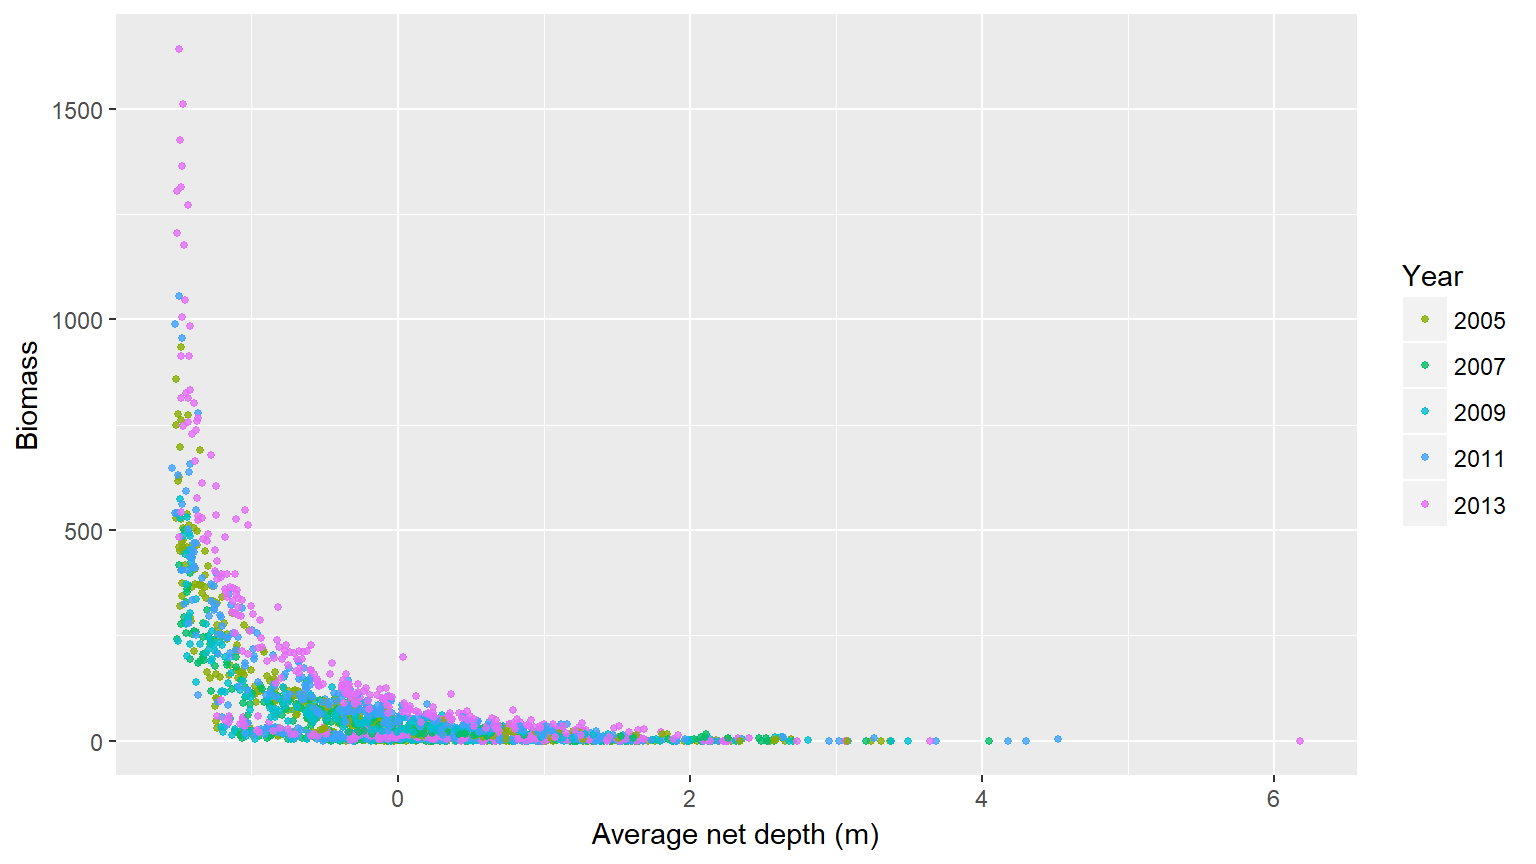
\includegraphics[width=.9\linewidth]{figure/sp_discrete_color_hue3b-1} 

}



\end{knitrout}
\end{frame}

%%%%%%%%%%%%%%%%%%%%%%%
\subsubsection{\lstinline{scale_color_brewer}}

\begin{frame}[fragile]{Discrete color scale: brewer palettes}
\vspace{-0.5cm}
\begin{center}
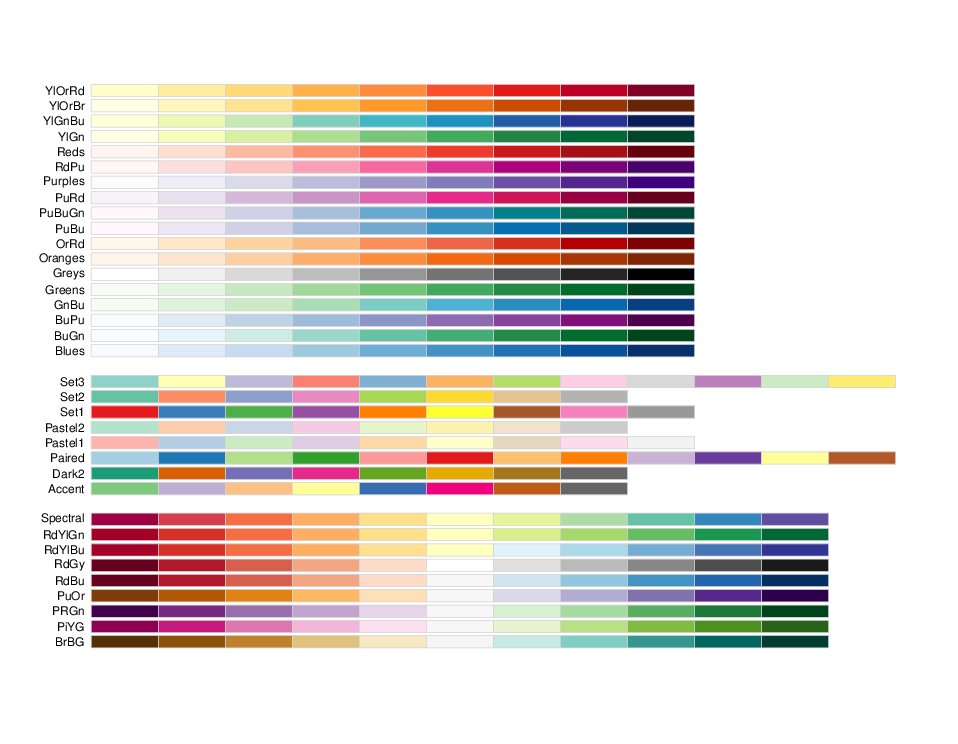
\includegraphics[scale=0.35]{colorbrewer_names.png}
\end{center}
\end{frame}

\begin{frame}[fragile]{Discrete color scale: brewer palette}
\begin{knitrout}\footnotesize
\definecolor{shadecolor}{rgb}{0.969, 0.969, 0.969}\color{fgcolor}\begin{kframe}
\begin{alltt}
\hlstd{sp_c_brewer} \hlkwb{<-} \hlstd{sp_c} \hlopt{+}
  \hlkwd{scale_color_brewer}\hlstd{(}\hlkwc{name}\hlstd{=}\hlstr{'Year'}\hlstd{,} \hlkwc{palette}\hlstd{=}\hlstr{"Dark2"}\hlstd{)}
\hlkwd{print}\hlstd{(sp_c_brewer)}
\end{alltt}
\end{kframe}

{\centering 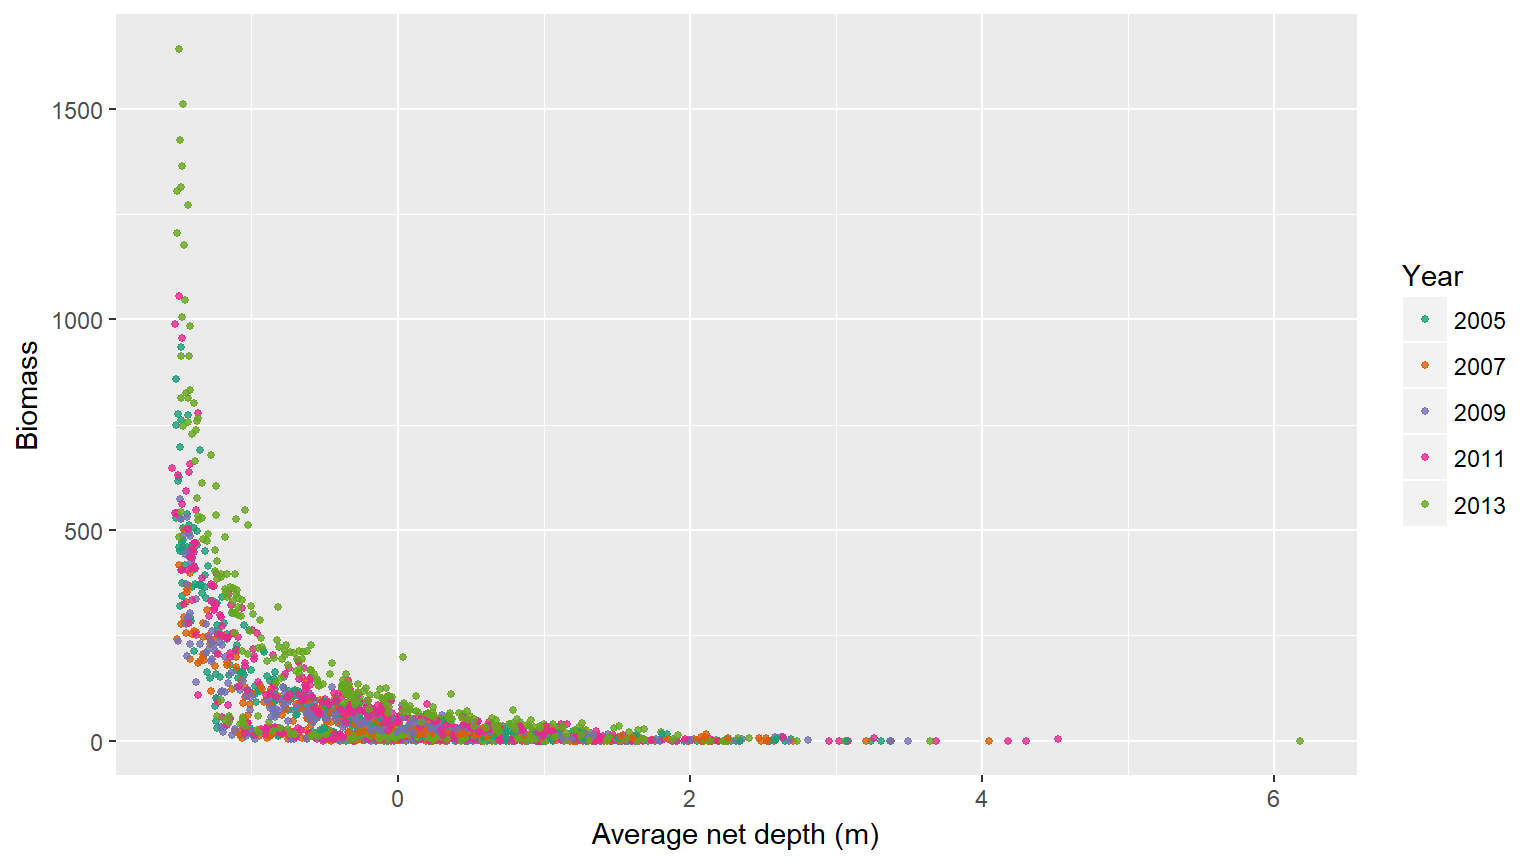
\includegraphics[width=.9\linewidth]{figure/sp_discrete_color4-1} 

}



\end{knitrout}
\end{frame}


\begin{frame}[fragile]{Discrete color scale: brewer palette}
\begin{knitrout}\footnotesize
\definecolor{shadecolor}{rgb}{0.969, 0.969, 0.969}\color{fgcolor}\begin{kframe}
\begin{alltt}
\hlstd{sp_c_brewer} \hlkwb{<-} \hlstd{sp_c} \hlopt{+}
  \hlkwd{scale_color_brewer}\hlstd{(}\hlkwc{name}\hlstd{=}\hlstr{'Year'}\hlstd{,} \hlkwc{palette}\hlstd{=}\hlstr{"Set1"}\hlstd{)}
\hlkwd{print}\hlstd{(sp_c_brewer)}
\end{alltt}
\end{kframe}

{\centering 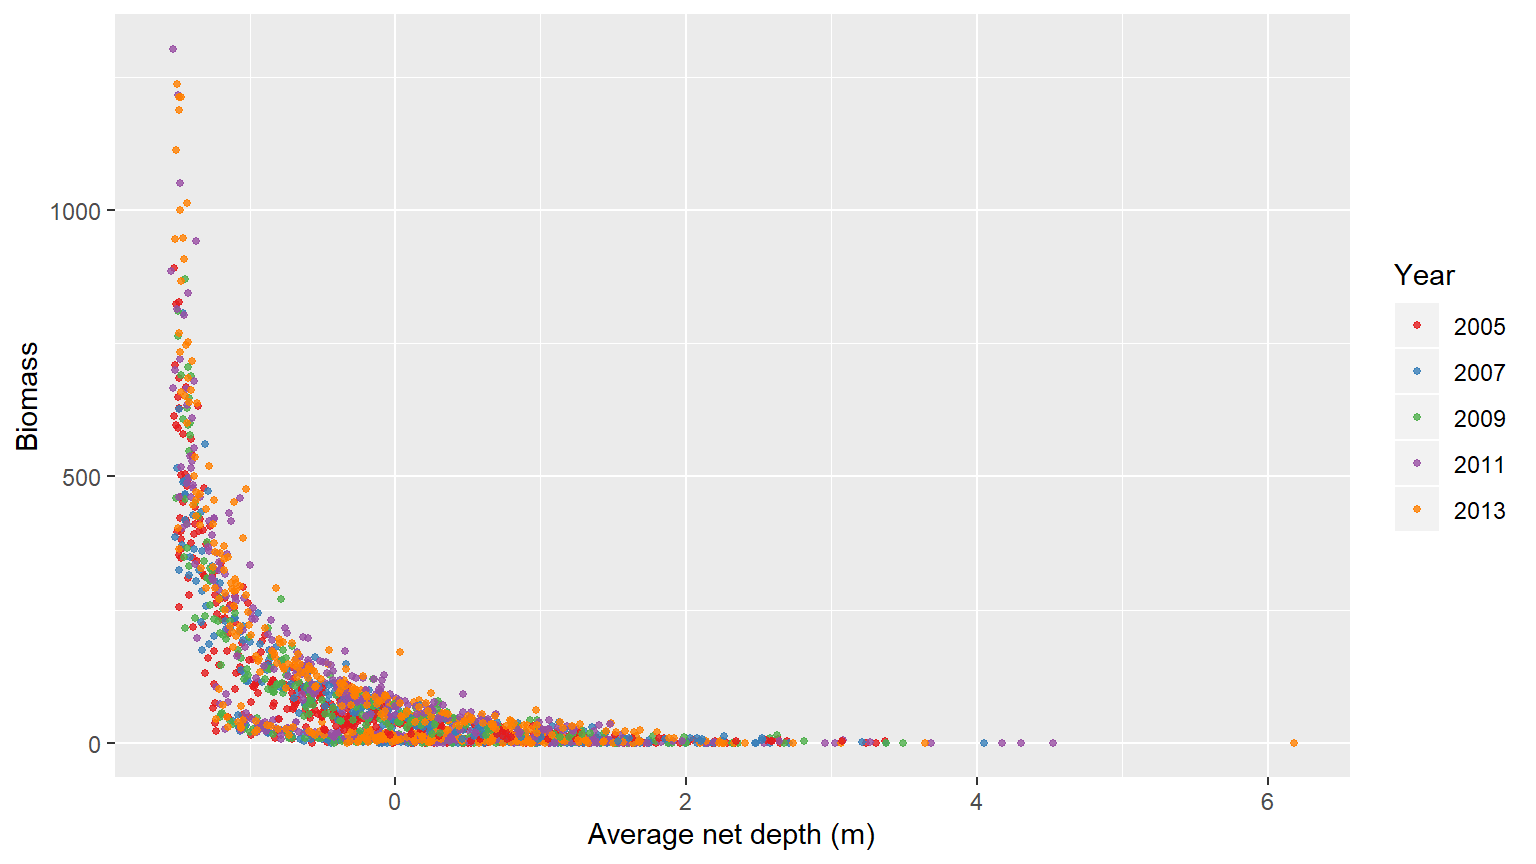
\includegraphics[width=.9\linewidth]{figure/sp_discrete_color4b-1} 

}



\end{knitrout}
\end{frame}

%%%%%%%%%%%%%%%%%%%%%%%
\subsubsection{wesanderson palettes}

\begin{frame}[fragile]{Discrete color scale: wesanderson palettes}
\begin{knitrout}\footnotesize
\definecolor{shadecolor}{rgb}{0.969, 0.969, 0.969}\color{fgcolor}\begin{kframe}
\begin{alltt}
\hlkwd{library}\hlstd{(wesanderson)}
\end{alltt}
\end{kframe}
\end{knitrout}
\begin{center}
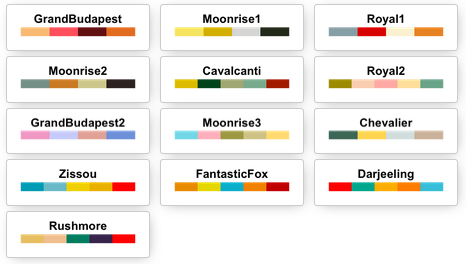
\includegraphics[scale=0.5]{wesanderson-color.png}
\end{center}

Other resources: 
\begin{itemize}
\item \url{http://www.stat.columbia.edu/~tzheng/files/Rcolor.pdf}
\item \url{http://research.stowers-institute.org/efg/R/Color/Chart/ColorChart.pdf}
\end{itemize}
\end{frame}


\begin{frame}[fragile]{Discrete color scale: wesanderson palettes}
\begin{knitrout}\footnotesize
\definecolor{shadecolor}{rgb}{0.969, 0.969, 0.969}\color{fgcolor}\begin{kframe}
\begin{alltt}
\hlstd{sp_c_wanderson} \hlkwb{<-} \hlstd{sp_c} \hlopt{+}
  \hlkwd{scale_color_manual}\hlstd{(}\hlkwc{name}\hlstd{=}\hlstr{'Year'}\hlstd{,} \hlkwc{values}\hlstd{=}\hlkwd{wes_palette}\hlstd{(}\hlkwc{name}\hlstd{=}\hlstr{"Darjeeling"}\hlstd{))}
\hlkwd{print}\hlstd{(sp_c_wanderson)}
\end{alltt}
\end{kframe}

{\centering 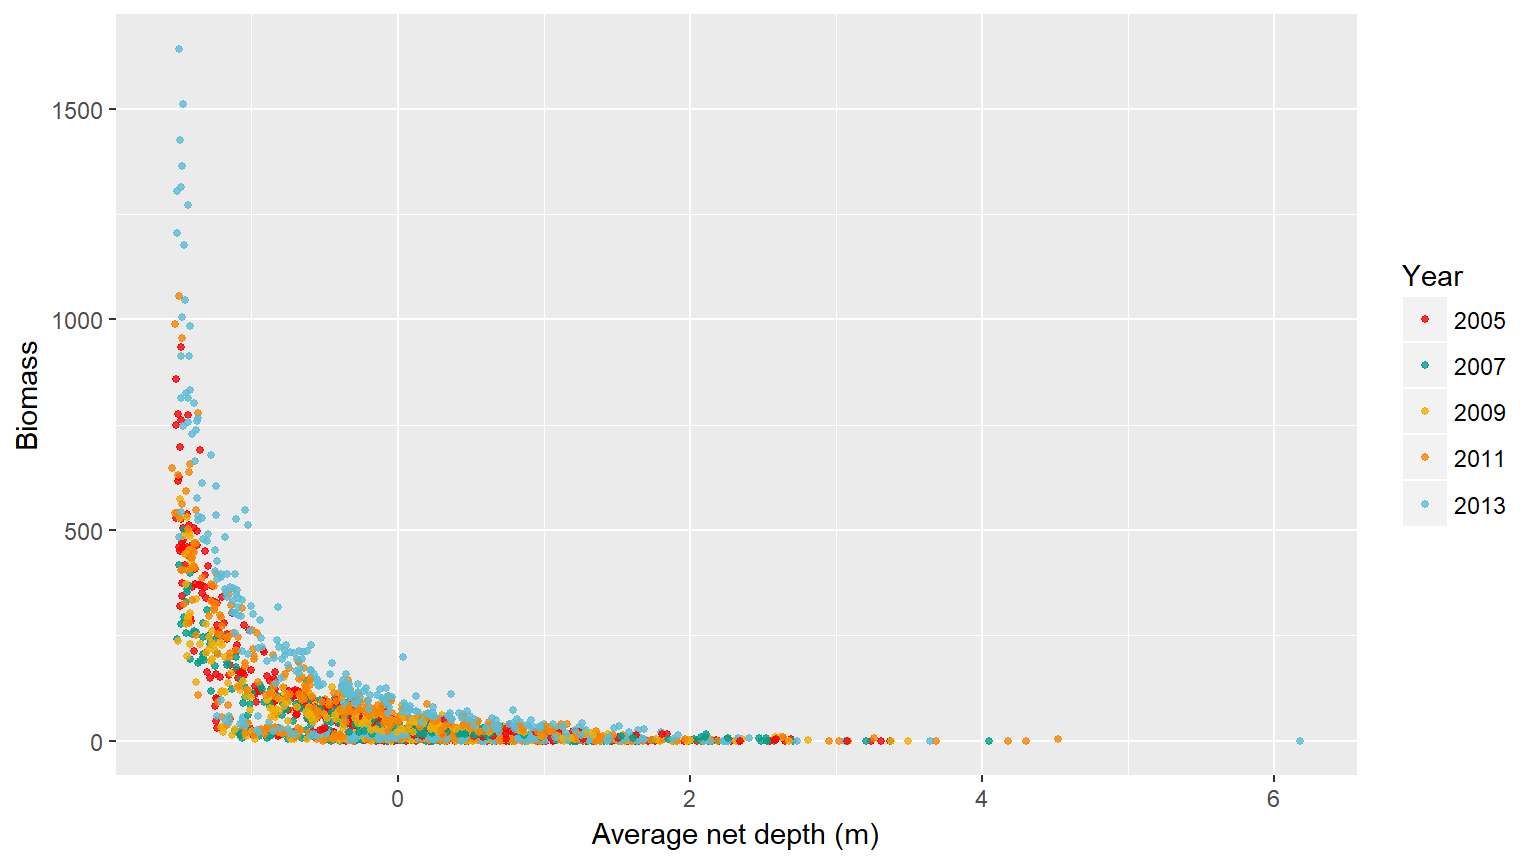
\includegraphics[width=.9\linewidth]{figure/sp_discrete_color_wa2-1} 

}



\end{knitrout}
\end{frame}

%%%%%%%%%%%%%%%%%%%%%%%
\subsubsection{\lstinline{scale_color_grey}}
\begin{frame}[fragile]{Discrete color scale: \lstinline{scale_color_grey}}
\begin{knitrout}\footnotesize
\definecolor{shadecolor}{rgb}{0.969, 0.969, 0.969}\color{fgcolor}\begin{kframe}
\begin{alltt}
\hlstd{sp_c_grey} \hlkwb{<-} \hlstd{sp_c} \hlopt{+}
  \hlkwd{scale_color_grey}\hlstd{(}\hlkwc{name}\hlstd{=}\hlstr{'Year'}\hlstd{)}
\hlkwd{print}\hlstd{(sp_c_grey)}
\end{alltt}
\end{kframe}

{\centering 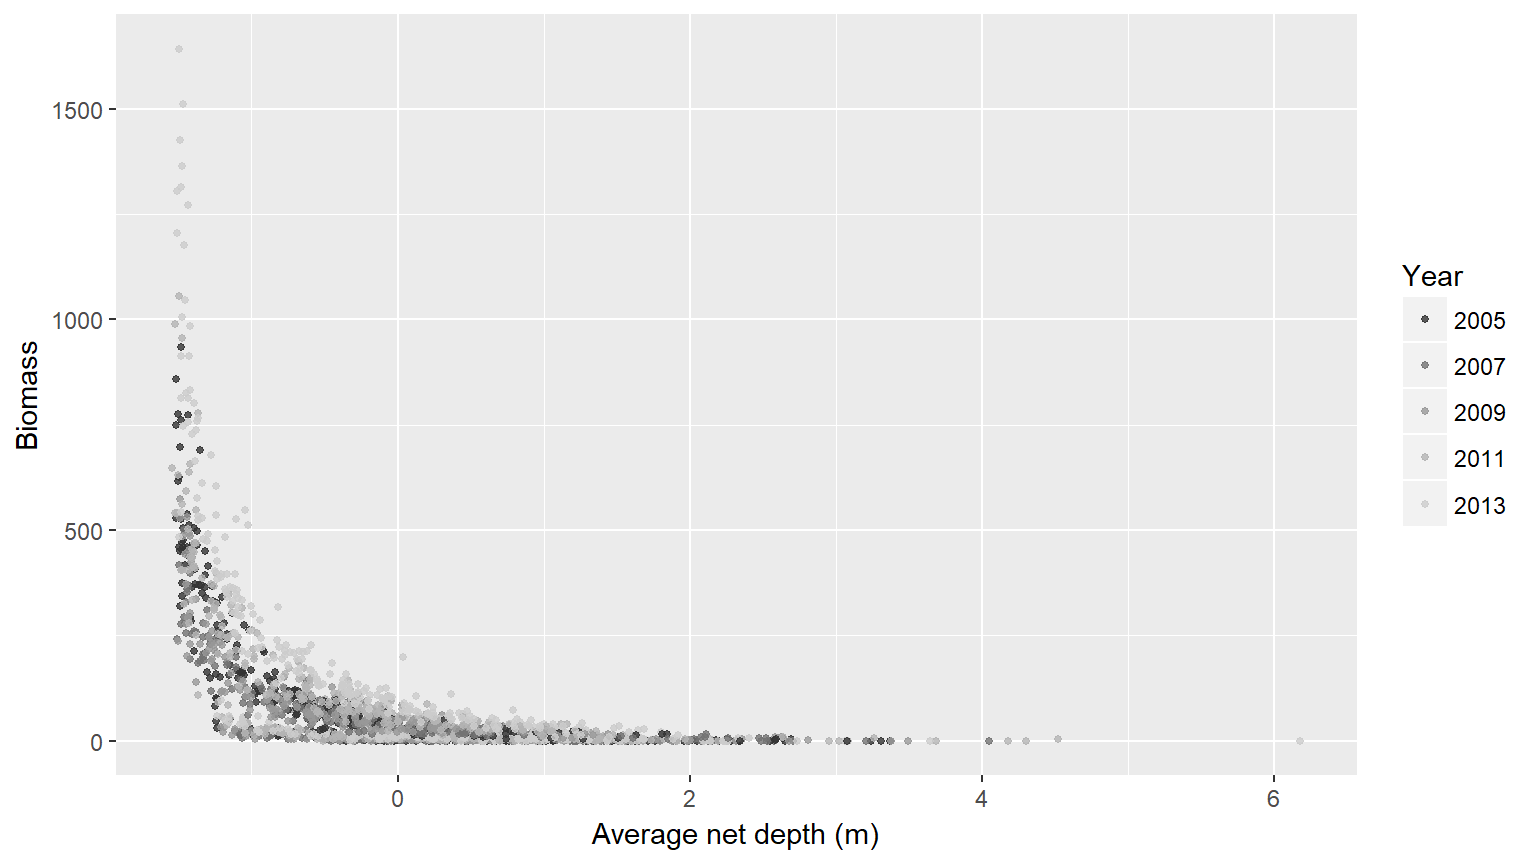
\includegraphics[width=.9\linewidth]{figure/sp_discrete_color5-1} 

}



\end{knitrout}
\end{frame}


\begin{frame}[fragile]{Discrete color scale: \lstinline{scale_color_grey}}
\begin{knitrout}\footnotesize
\definecolor{shadecolor}{rgb}{0.969, 0.969, 0.969}\color{fgcolor}\begin{kframe}
\begin{alltt}
\hlstd{sp_c_grey} \hlkwb{<-} \hlstd{sp_c} \hlopt{+}
  \hlkwd{scale_color_grey}\hlstd{(}\hlkwc{name}\hlstd{=}\hlstr{'Year'}\hlstd{,} \hlkwc{start}\hlstd{=}\hlnum{0.8}\hlstd{,} \hlkwc{end}\hlstd{=}\hlnum{0.2}\hlstd{)}
\hlkwd{print}\hlstd{(sp_c_grey)}
\end{alltt}
\end{kframe}

{\centering 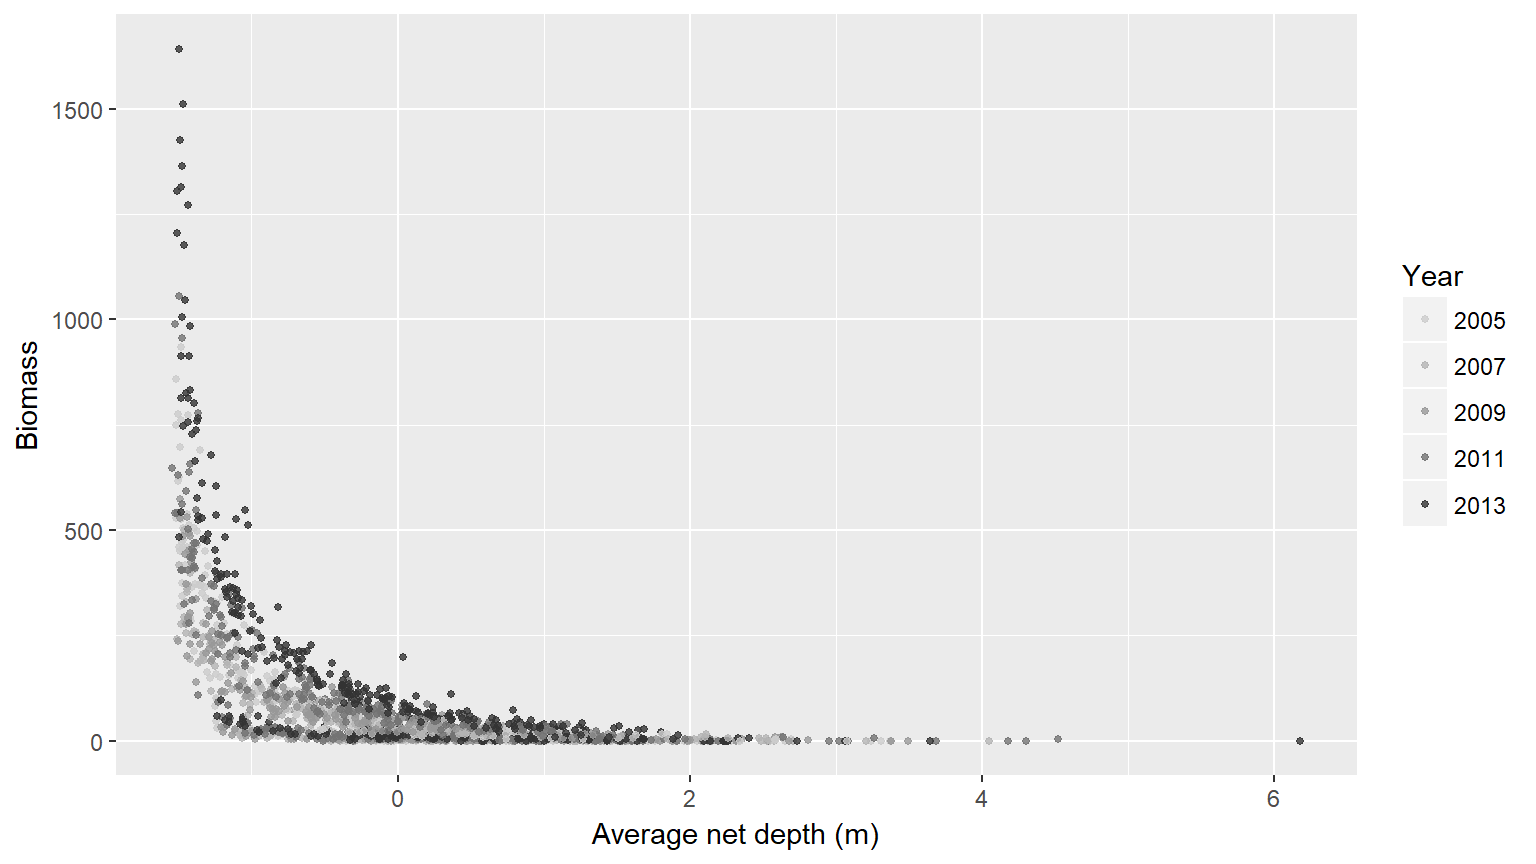
\includegraphics[width=.9\linewidth]{figure/sp_discrete_color6-1} 

}



\end{knitrout}
\end{frame}

%%%%%%%%%%%%%%%%%%%%%%%
\subsubsection{manual scale}

\begin{frame}[fragile]{Discrete color scale: manual}
\begin{knitrout}\footnotesize
\definecolor{shadecolor}{rgb}{0.969, 0.969, 0.969}\color{fgcolor}\begin{kframe}
\begin{alltt}
\hlstd{sp_c_manual} \hlkwb{<-} \hlstd{sp_color} \hlopt{+}
  \hlkwd{scale_color_manual}\hlstd{(}\hlkwc{name}\hlstd{=}\hlstr{'Area'}\hlstd{,} \hlkwc{values}\hlstd{=}\hlkwd{c}\hlstd{(}\hlstr{"#E69F00"}\hlstd{,} \hlstr{"#56B4E9"}\hlstd{))}
\hlkwd{print}\hlstd{(sp_c_manual)}
\end{alltt}
\end{kframe}

{\centering 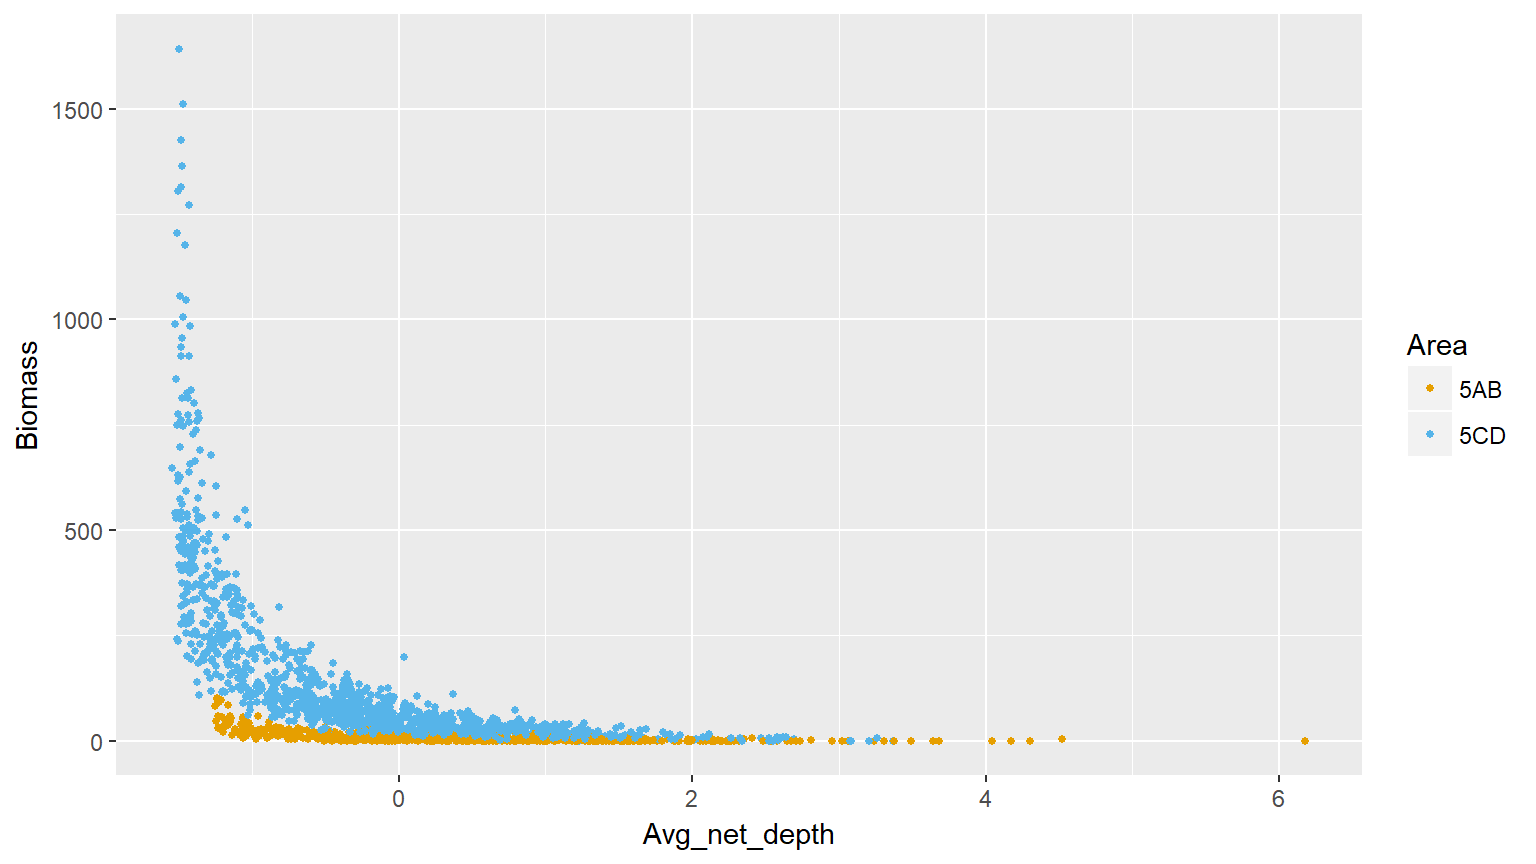
\includegraphics[width=.9\linewidth]{figure/sp_discrete_color2-1} 

}



\end{knitrout}
\end{frame}




\begin{frame}[fragile]{Color scale: make your own}
A color-blind palette:
\begin{knitrout}\footnotesize
\definecolor{shadecolor}{rgb}{0.969, 0.969, 0.969}\color{fgcolor}\begin{kframe}
\begin{alltt}
\hlstd{cb_palette_black} \hlkwb{<-} \hlkwd{c}\hlstd{(}\hlstr{"#E69F00"}\hlstd{,} \hlstr{"#56B4E9"}\hlstd{,} \hlstr{"#009E73"}\hlstd{,} \hlstr{"#F0E442"}\hlstd{,}
                      \hlstr{"#0072B2"}\hlstd{,} \hlstr{"#D55E00"}\hlstd{,} \hlstr{"#CC79A7"}\hlstd{,} \hlstr{"#000000"}\hlstd{)}
\end{alltt}
\end{kframe}
\end{knitrout}
Or create your own gradient palette function with 2 or more colors:
\begin{knitrout}\footnotesize
\definecolor{shadecolor}{rgb}{0.969, 0.969, 0.969}\color{fgcolor}\begin{kframe}
\begin{alltt}
\hlcom{## Palette from white-grey to red to black}
\hlstd{Palette_grb} \hlkwb{<-} \hlkwd{colorRampPalette}\hlstd{(}\hlkwd{c}\hlstd{(}\hlkwd{colors}\hlstd{()[}\hlnum{139}\hlstd{],} \hlcom{# green}
                                  \hlkwd{colors}\hlstd{()[}\hlnum{554}\hlstd{],} \hlcom{# red}
                                  \hlkwd{colors}\hlstd{()[}\hlnum{153}\hlstd{])} \hlcom{# black}
                \hlstd{)}
\end{alltt}
\end{kframe}
\end{knitrout}
\end{frame}

\begin{frame}[fragile]{Discrete color scale: manual}
\begin{knitrout}\footnotesize
\definecolor{shadecolor}{rgb}{0.969, 0.969, 0.969}\color{fgcolor}\begin{kframe}
\begin{alltt}
\hlstd{sp_color_cb} \hlkwb{<-} \hlstd{sp_c} \hlopt{+}
  \hlkwd{scale_color_manual}\hlstd{(}\hlkwc{name}\hlstd{=}\hlstr{'Year'}\hlstd{,} \hlkwc{values} \hlstd{= cb_palette_black)}
\hlkwd{print}\hlstd{(sp_color_cb)}
\end{alltt}
\end{kframe}

{\centering 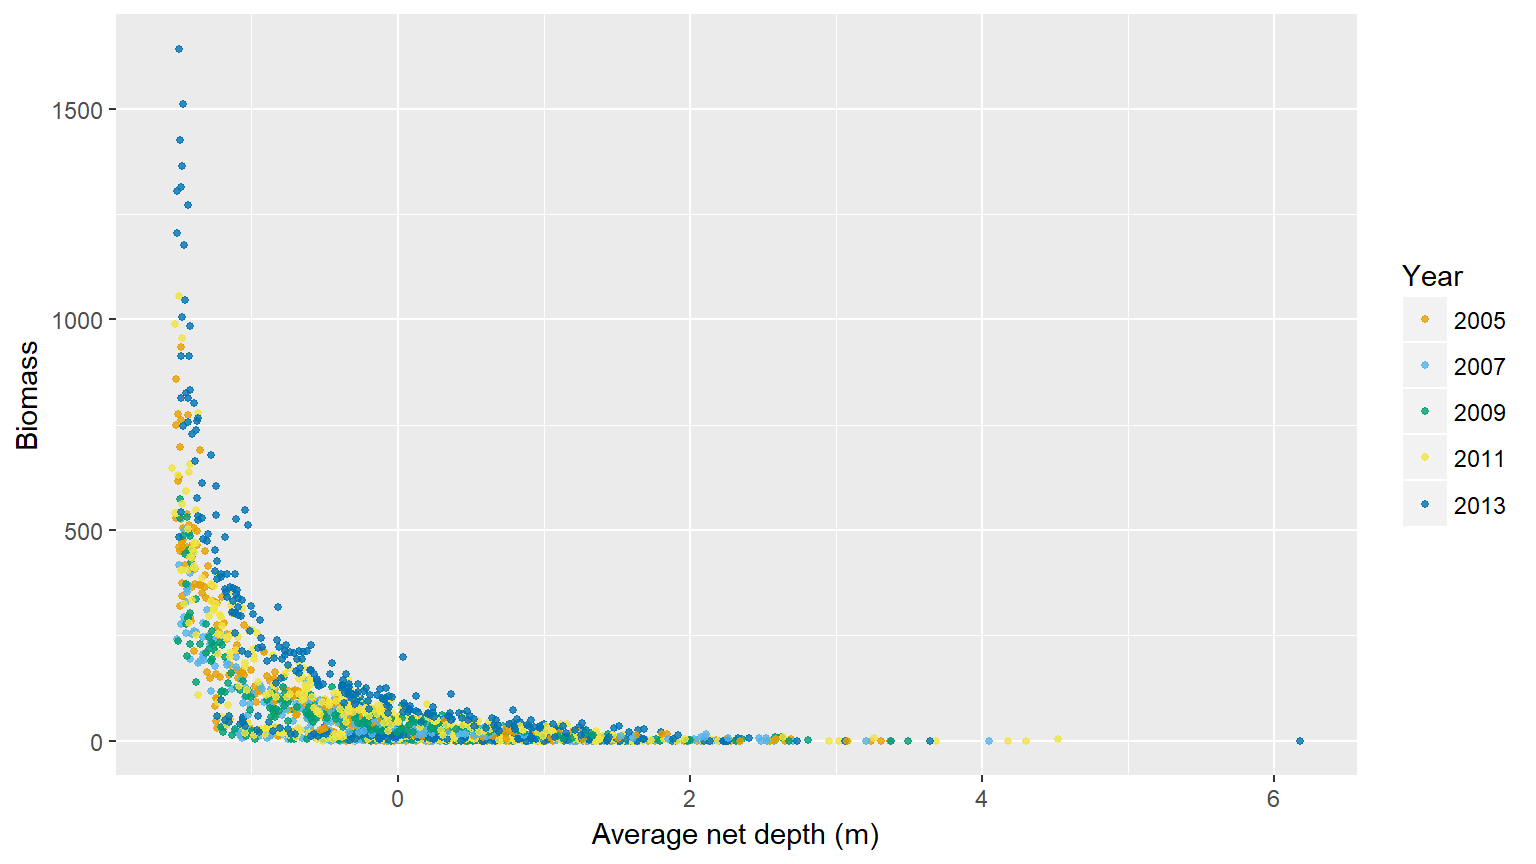
\includegraphics[width=.9\linewidth]{figure/sp_discrete_colorcb-1} 

}



\end{knitrout}
\end{frame}

\begin{frame}[fragile]{Discrete color scale: manual}
\begin{knitrout}\footnotesize
\definecolor{shadecolor}{rgb}{0.969, 0.969, 0.969}\color{fgcolor}\begin{kframe}
\begin{alltt}
\hlstd{sp_color_own} \hlkwb{<-} \hlstd{sp_c} \hlopt{+}
  \hlkwd{scale_color_manual}\hlstd{(}\hlkwc{name}\hlstd{=}\hlstr{'Year'}\hlstd{,} \hlkwc{values} \hlstd{=} \hlkwd{Palette_grb}\hlstd{(nYear))}
\hlkwd{print}\hlstd{(sp_color_own)}
\end{alltt}
\end{kframe}

{\centering 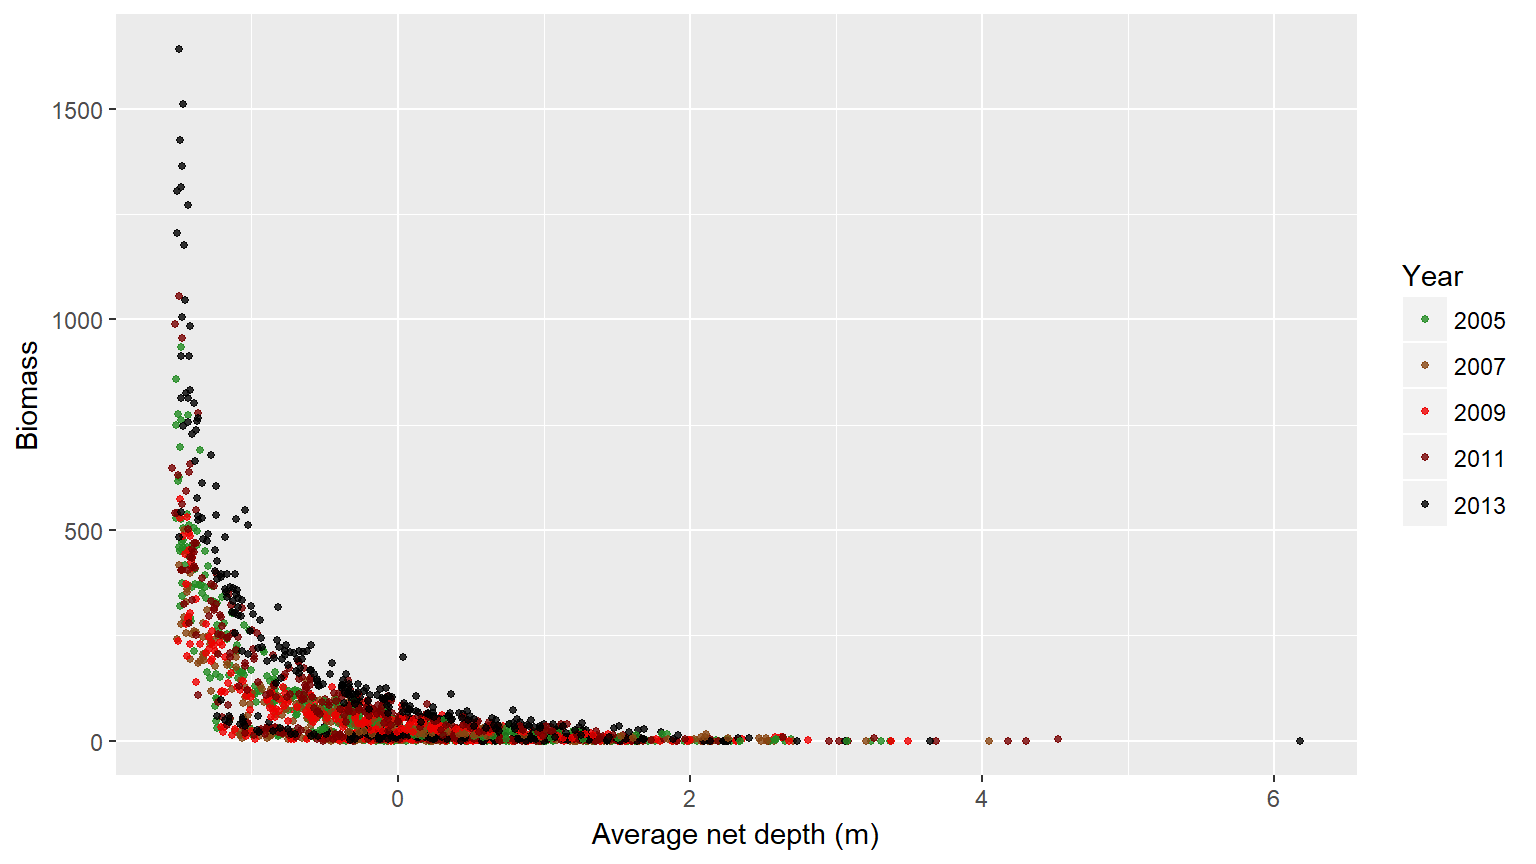
\includegraphics[width=.9\linewidth]{figure/sp_discrete_colorown-1} 

}



\end{knitrout}
\end{frame}


%%%%%%%%%%%%%%%%%%%%%%%
\subsection{Colors for continuous variables}

\begin{frame}[fragile]{Continuous color scale}
\begin{knitrout}\footnotesize
\definecolor{shadecolor}{rgb}{0.969, 0.969, 0.969}\color{fgcolor}\begin{kframe}
\begin{alltt}
\hlstd{sp_cc} \hlkwb{<-} \hlkwd{ggplot}\hlstd{(df_data,} \hlkwd{aes}\hlstd{(}\hlkwc{x}\hlstd{=Avg_net_temp,} \hlkwc{y}\hlstd{=Avg_net_depth))} \hlopt{+}
  \hlkwd{geom_point}\hlstd{(}\hlkwc{alpha}\hlstd{=}\hlnum{0.8}\hlstd{,} \hlkwc{size}\hlstd{=}\hlnum{1}\hlstd{,} \hlkwd{aes}\hlstd{(}\hlkwc{colour}\hlstd{=Biomass))} \hlopt{+}
  \hlkwd{xlab}\hlstd{(}\hlstr{'Average net temperature (C)'}\hlstd{)} \hlopt{+} \hlkwd{ylab}\hlstd{(}\hlstr{'Average net depth (m)'}\hlstd{)}
\hlkwd{print}\hlstd{(sp_cc)}
\end{alltt}
\end{kframe}

{\centering 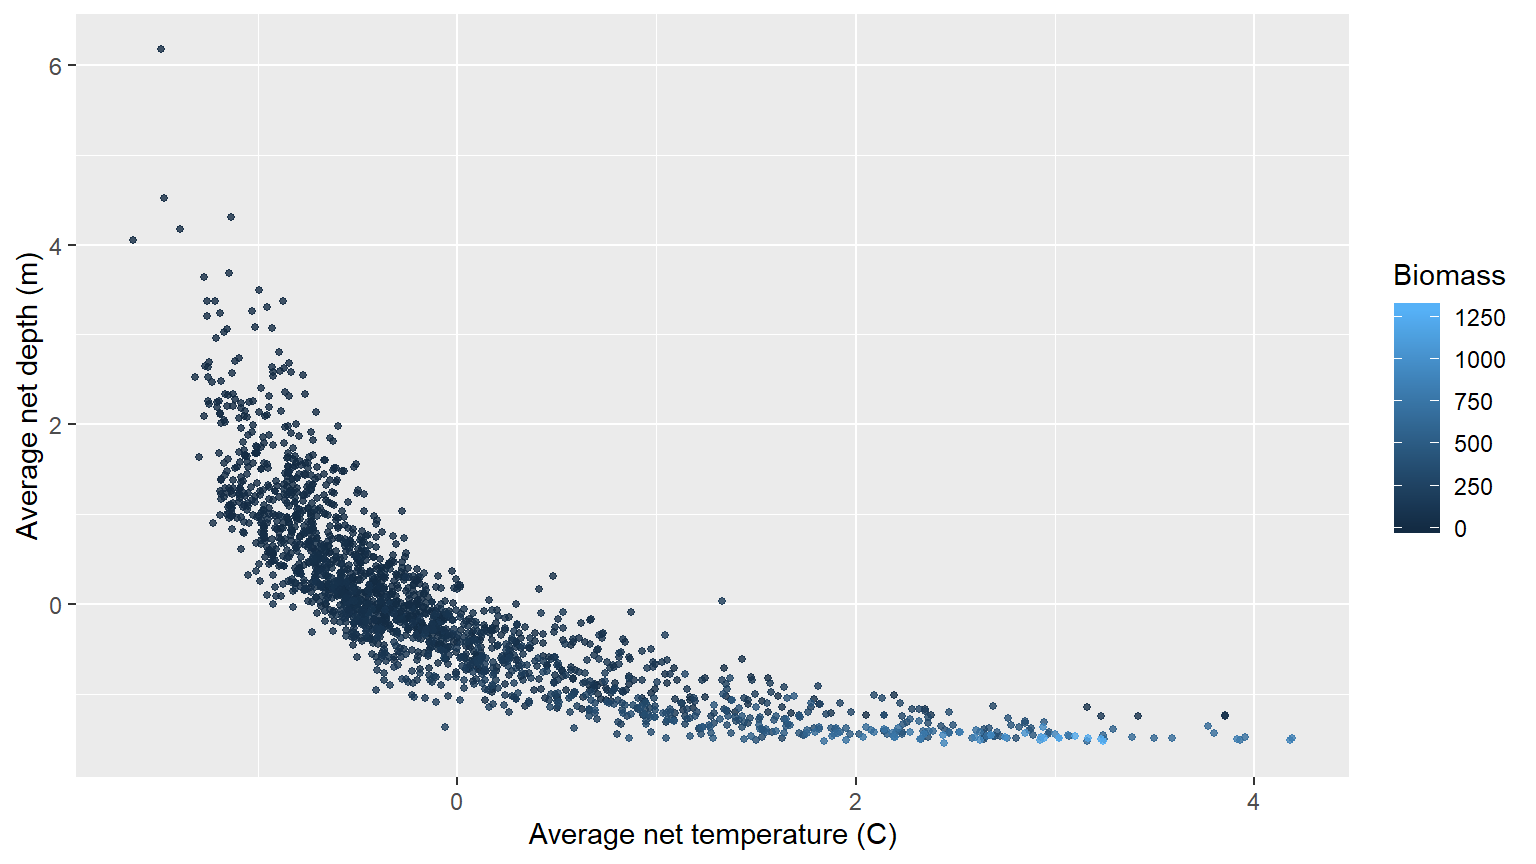
\includegraphics[width=.9\linewidth]{figure/sp_continuous_color1-1} 

}



\end{knitrout}
\end{frame}

\begin{frame}[fragile]{Continuous color scale: choose color}
\begin{knitrout}\footnotesize
\definecolor{shadecolor}{rgb}{0.969, 0.969, 0.969}\color{fgcolor}\begin{kframe}
\begin{alltt}
\hlstd{sp_cc2} \hlkwb{<-} \hlstd{sp_cc} \hlopt{+}
  \hlkwd{scale_colour_gradient}\hlstd{(}\hlkwc{low} \hlstd{=} \hlstr{'blue'}\hlstd{,} \hlkwc{high} \hlstd{=} \hlstr{'red'}\hlstd{)}
\hlkwd{print}\hlstd{(sp_cc2)}
\end{alltt}
\end{kframe}

{\centering 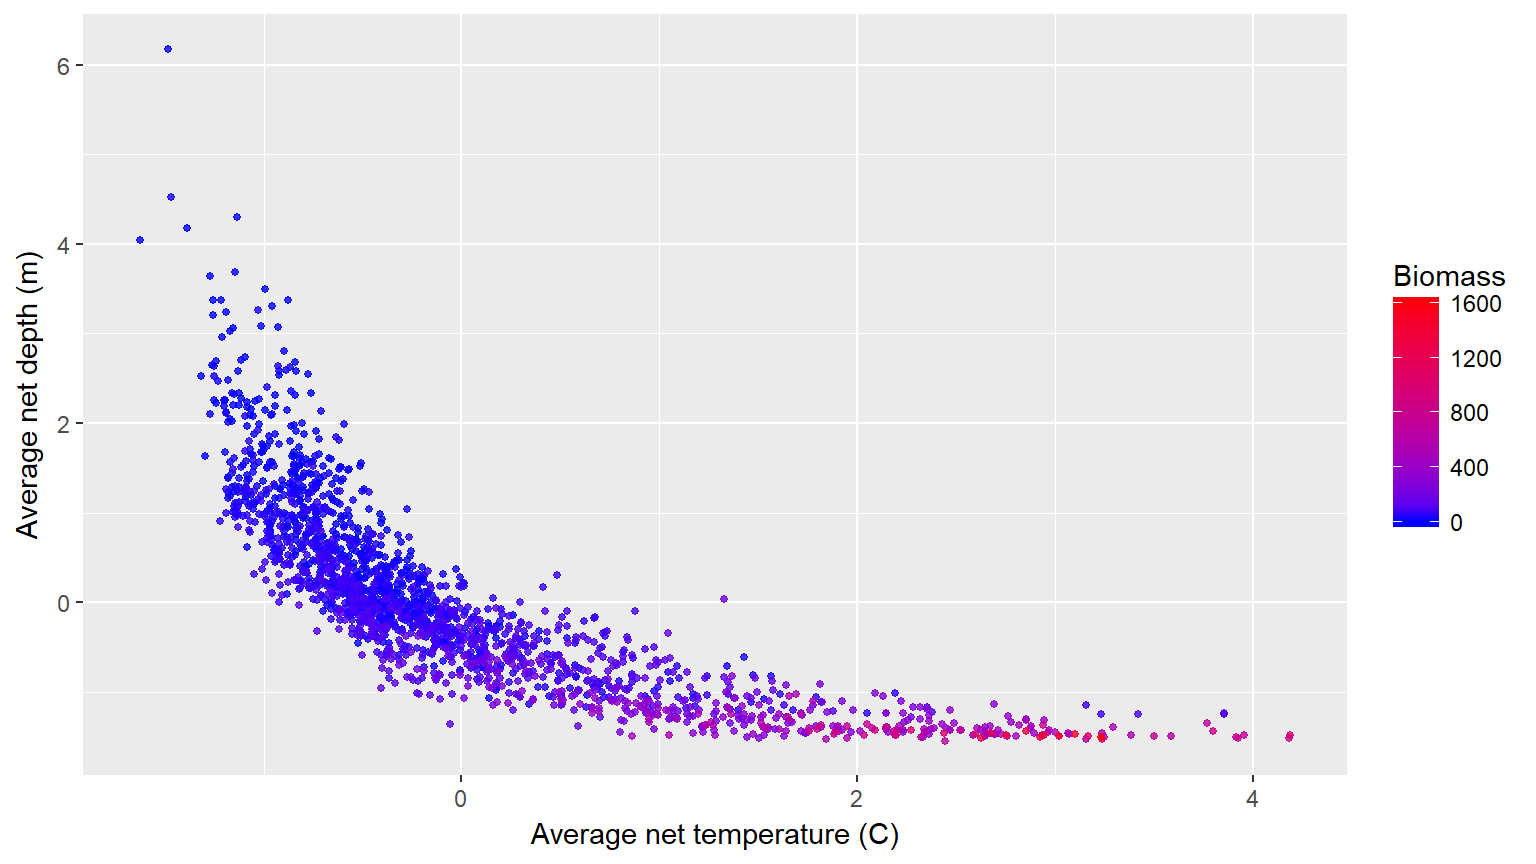
\includegraphics[width=.9\linewidth]{figure/sp_continuous_color2-1} 

}



\end{knitrout}
\end{frame}

\begin{frame}[fragile]{Continuous color scale: divergent scale}
\begin{knitrout}\footnotesize
\definecolor{shadecolor}{rgb}{0.969, 0.969, 0.969}\color{fgcolor}\begin{kframe}
\begin{alltt}
\hlstd{sp_cc_div} \hlkwb{<-} \hlstd{sp_cc} \hlopt{+}
  \hlkwd{scale_colour_gradient2}\hlstd{(}\hlkwc{midpoint} \hlstd{=} \hlnum{100}\hlstd{,}
                         \hlkwc{low} \hlstd{=} \hlstr{'blue'}\hlstd{,} \hlkwc{high} \hlstd{=} \hlstr{'red'}\hlstd{,} \hlkwc{mid} \hlstd{=} \hlkwd{muted}\hlstd{(}\hlstr{'green'}\hlstd{))}
\hlkwd{print}\hlstd{(sp_cc_div)}
\end{alltt}
\end{kframe}

{\centering 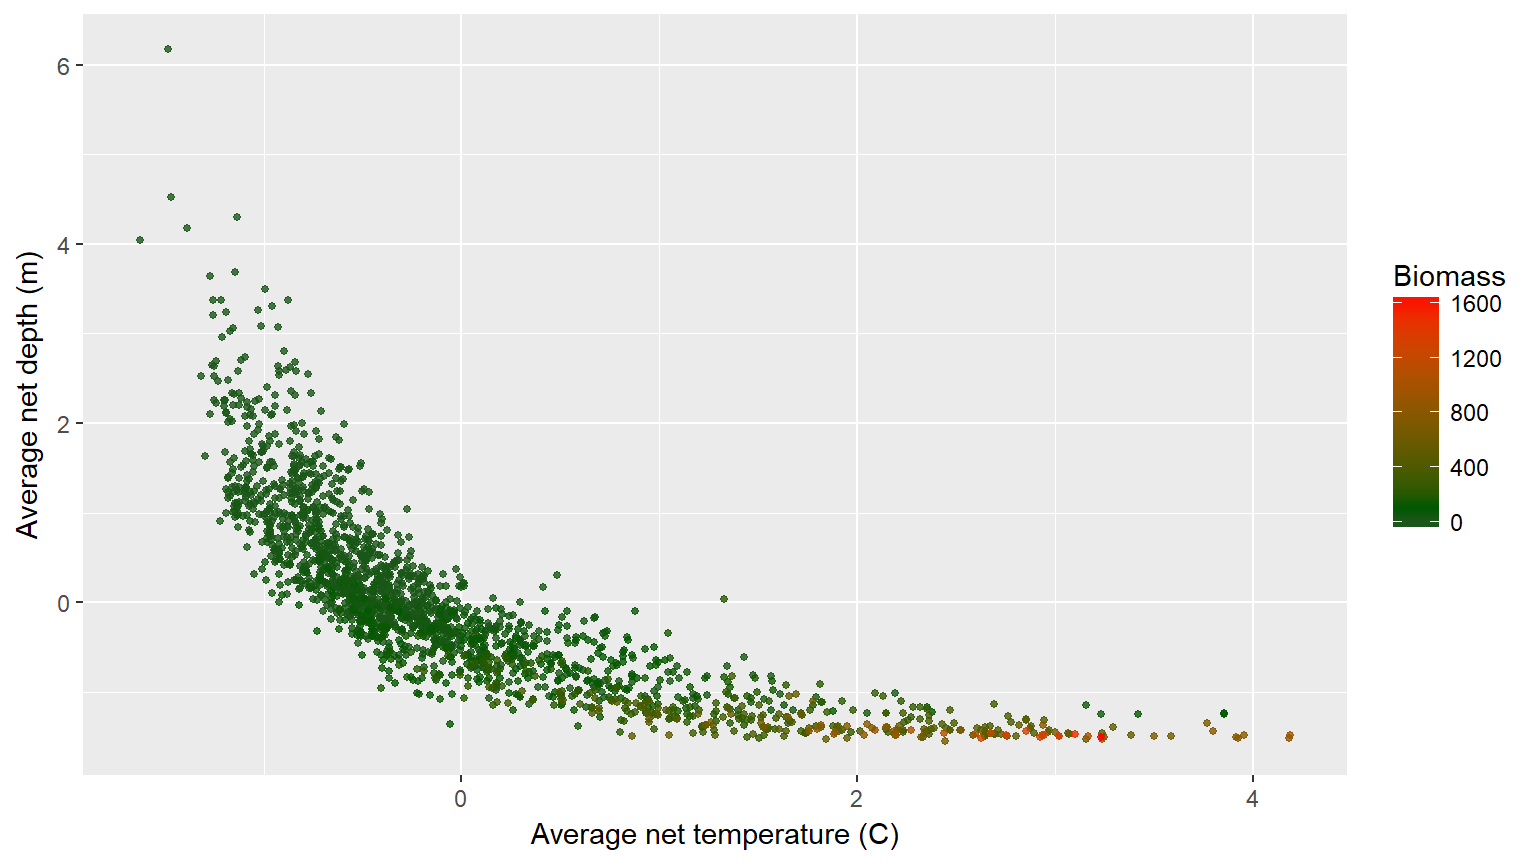
\includegraphics[width=.9\linewidth]{figure/sp_continuous_color3-1} 

}



\end{knitrout}
\end{frame}

\begin{frame}[fragile]{Continuous color scale: rainbow scale}
\begin{knitrout}\footnotesize
\definecolor{shadecolor}{rgb}{0.969, 0.969, 0.969}\color{fgcolor}\begin{kframe}
\begin{alltt}
\hlstd{sp_cc_own} \hlkwb{<-} \hlstd{sp_cc} \hlopt{+}
  \hlkwd{scale_color_gradientn}\hlstd{(}\hlkwc{colors} \hlstd{=} \hlkwd{rainbow}\hlstd{(}\hlnum{5}\hlstd{))}
\hlkwd{print}\hlstd{(sp_cc_own)}
\end{alltt}
\end{kframe}

{\centering 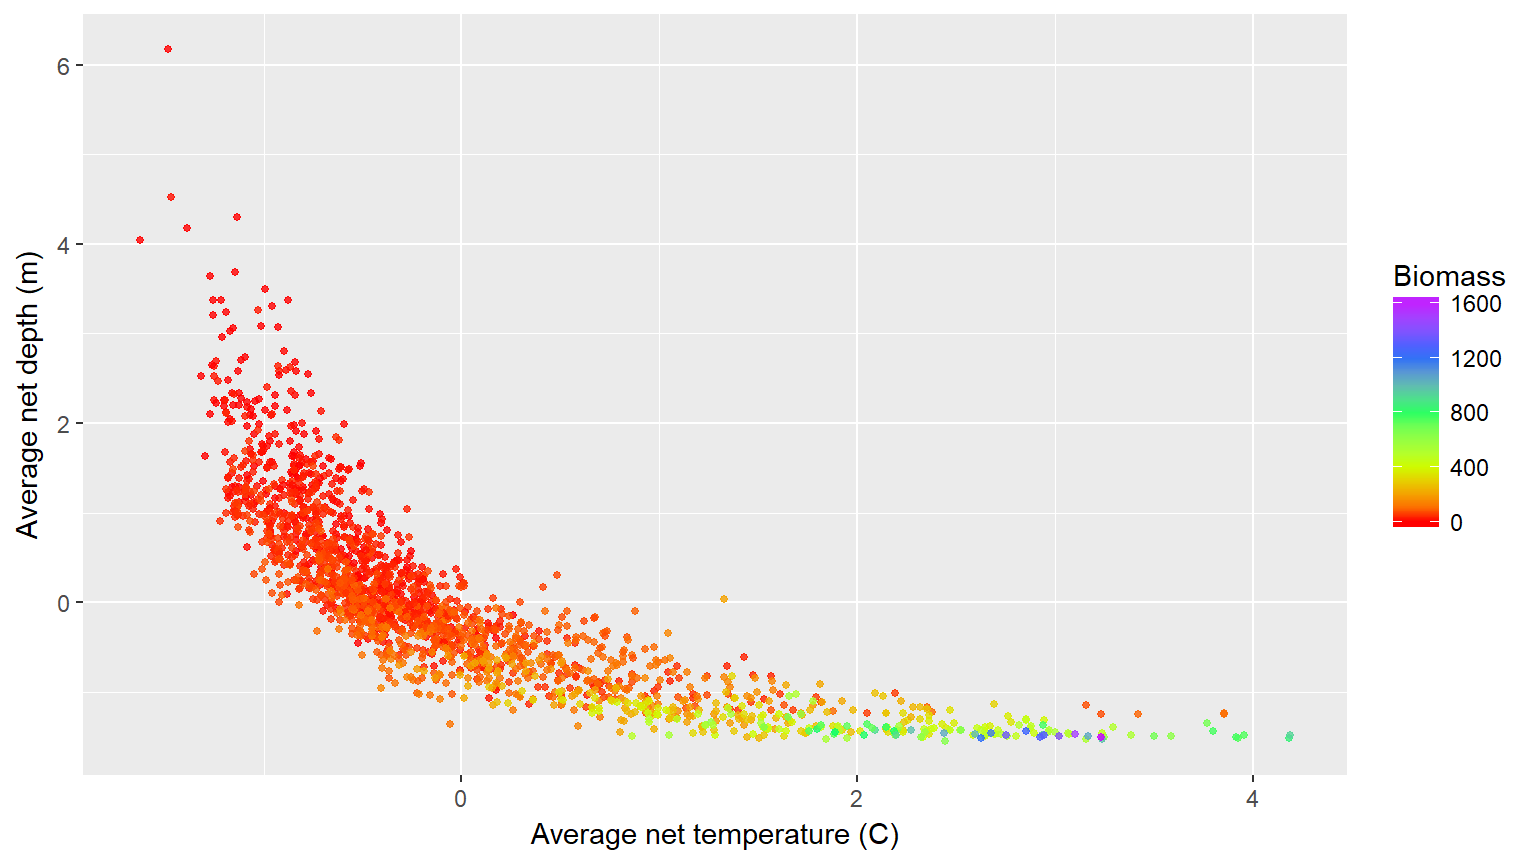
\includegraphics[width=.9\linewidth]{figure/sp_continuous_color4-1} 

}



\end{knitrout}
\end{frame}

\begin{frame}[fragile]{Continuous color scale: wesanderson scale}
\begin{knitrout}\footnotesize
\definecolor{shadecolor}{rgb}{0.969, 0.969, 0.969}\color{fgcolor}\begin{kframe}
\begin{alltt}
\hlstd{sp_cc_own} \hlkwb{<-} \hlstd{sp_cc} \hlopt{+}
  \hlkwd{scale_color_gradientn}\hlstd{(}\hlkwc{colors} \hlstd{=} \hlkwd{wes_palette}\hlstd{(}\hlkwc{n}\hlstd{=}\hlnum{5}\hlstd{,}
                                             \hlkwc{name}\hlstd{=}\hlstr{"Rushmore"}\hlstd{,}
                                             \hlkwc{type} \hlstd{=} \hlstr{'continuous'}\hlstd{))}
\hlkwd{print}\hlstd{(sp_cc_own)}
\end{alltt}
\end{kframe}

{\centering 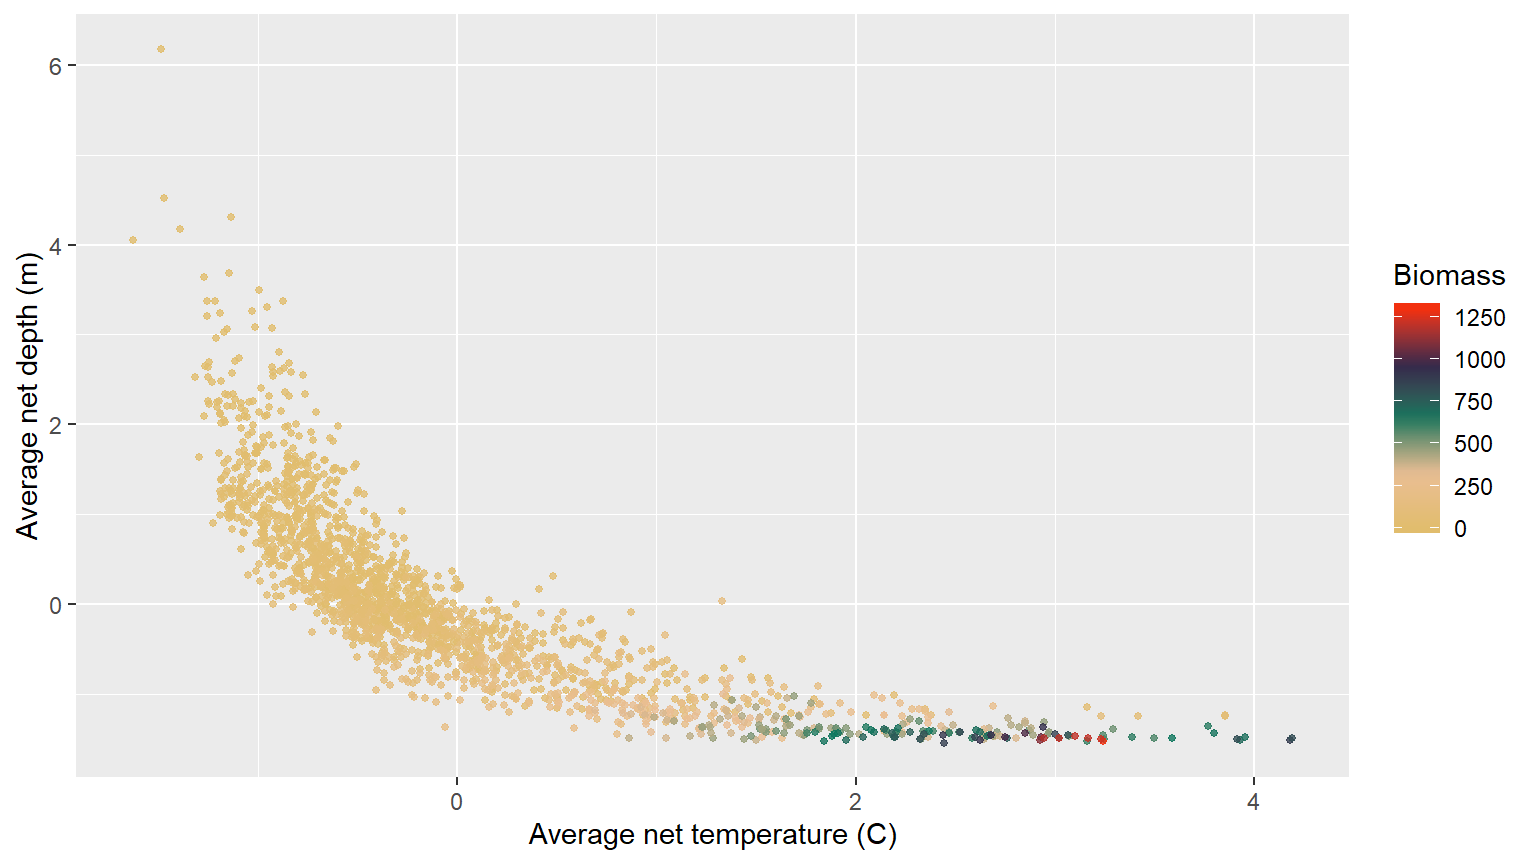
\includegraphics[width=.9\linewidth]{figure/sp_continuous_color5-1} 

}



\end{knitrout}
\end{frame}

\begin{frame}[fragile]{Continuous color scale: own scale}
\begin{knitrout}\footnotesize
\definecolor{shadecolor}{rgb}{0.969, 0.969, 0.969}\color{fgcolor}\begin{kframe}
\begin{alltt}
\hlstd{sp_cc_own} \hlkwb{<-} \hlstd{sp_cc} \hlopt{+}
  \hlkwd{scale_color_gradientn}\hlstd{(}\hlkwc{colors} \hlstd{=} \hlkwd{Palette_grb}\hlstd{(}\hlnum{10}\hlstd{))}
\hlkwd{print}\hlstd{(sp_cc_own)}
\end{alltt}
\end{kframe}

{\centering 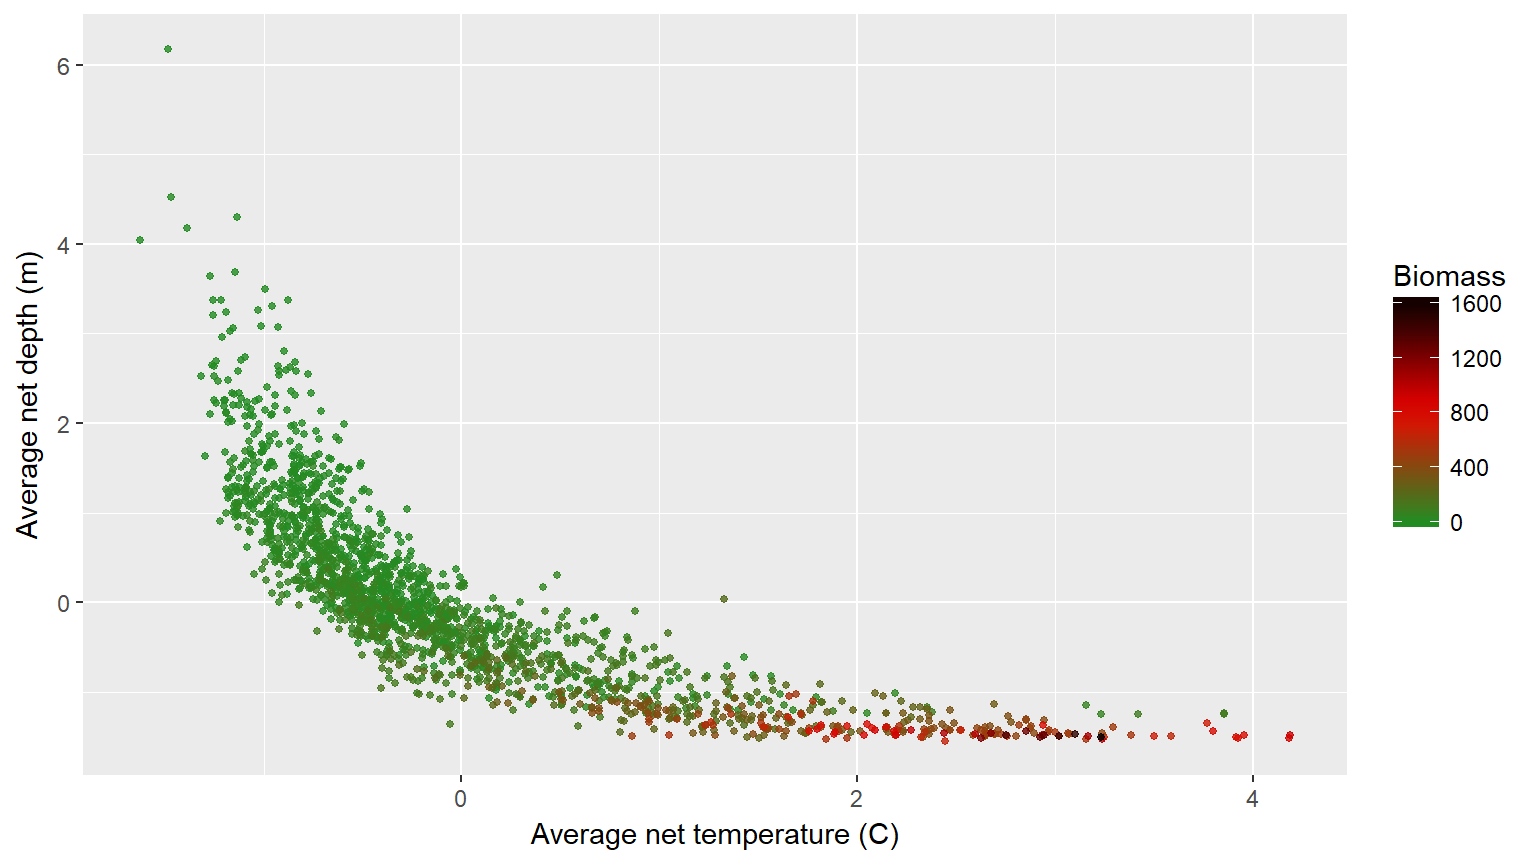
\includegraphics[width=.9\linewidth]{figure/sp_continuous_color6-1} 

}



\end{knitrout}
\end{frame}

\begin{frame}[fragile]{Continuous color scale: own scale}
\begin{knitrout}\footnotesize
\definecolor{shadecolor}{rgb}{0.969, 0.969, 0.969}\color{fgcolor}\begin{kframe}
\begin{alltt}
\hlstd{sp_cc_own} \hlkwb{<-} \hlstd{sp_cc} \hlopt{+}
  \hlkwd{scale_color_gradientn}\hlstd{(}\hlkwc{colors} \hlstd{=} \hlkwd{Palette_grb}\hlstd{(}\hlnum{3}\hlstd{))}
\hlkwd{print}\hlstd{(sp_cc_own)}
\end{alltt}
\end{kframe}

{\centering 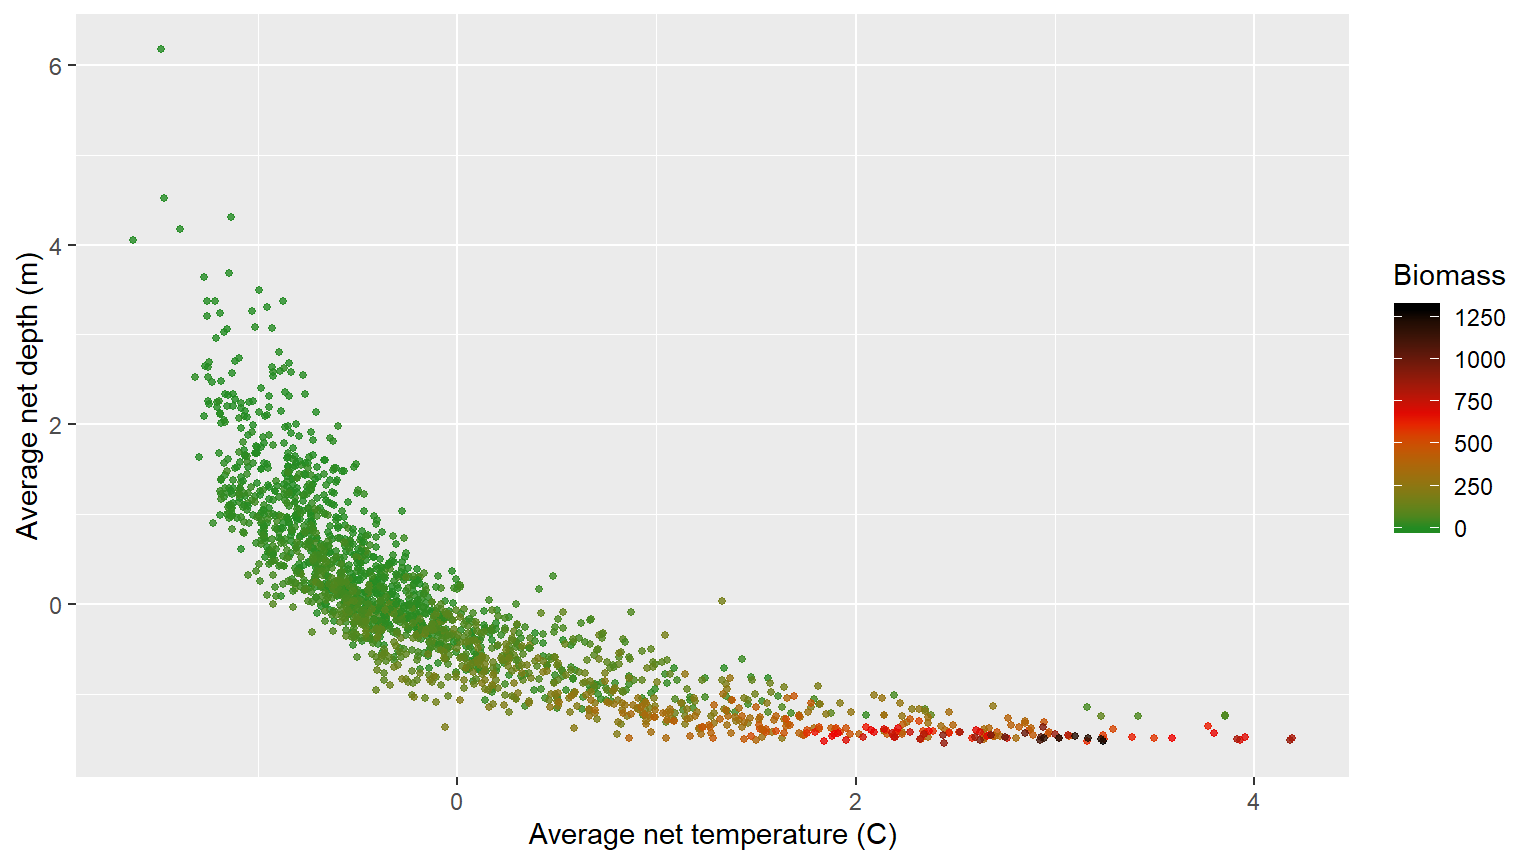
\includegraphics[width=.9\linewidth]{figure/sp_continuous_color7-1} 

}



\end{knitrout}
\end{frame}



%%%%%%%%%%%%%%%%%%%%%%%%%%%%%%%%%%%%%%%%%%%%%%%%%%%%%%%%%%%%%%%%%%%%%%%%%%%%%%%%
%% Time series
%%%%%%%%%%%%%%%%%%%%%%%%%%%%%%%%%%%%%%%%%%%%%%%%%%%%%%%%%%%%%%%%%%%%%%%%%%%%%%%%
\section{Time series}
\begin{frame}[fragile]{Time series}
\begin{knitrout}\footnotesize
\definecolor{shadecolor}{rgb}{0.969, 0.969, 0.969}\color{fgcolor}\begin{kframe}
\begin{alltt}
\hlstd{TSplot} \hlkwb{<-} \hlkwd{ggplot}\hlstd{(}\hlkwc{data}\hlstd{=df_data,} \hlkwd{aes}\hlstd{(}\hlkwc{x}\hlstd{=Date,} \hlkwc{y}\hlstd{=Biomass))} \hlopt{+}
  \hlkwd{geom_point}\hlstd{()} \hlopt{+} \hlkwd{ylim}\hlstd{(}\hlnum{0}\hlstd{,}\hlkwd{max}\hlstd{(df_data}\hlopt{$}\hlstd{Biomass))}
\hlkwd{print}\hlstd{(TSplot)}
\end{alltt}
\end{kframe}

{\centering 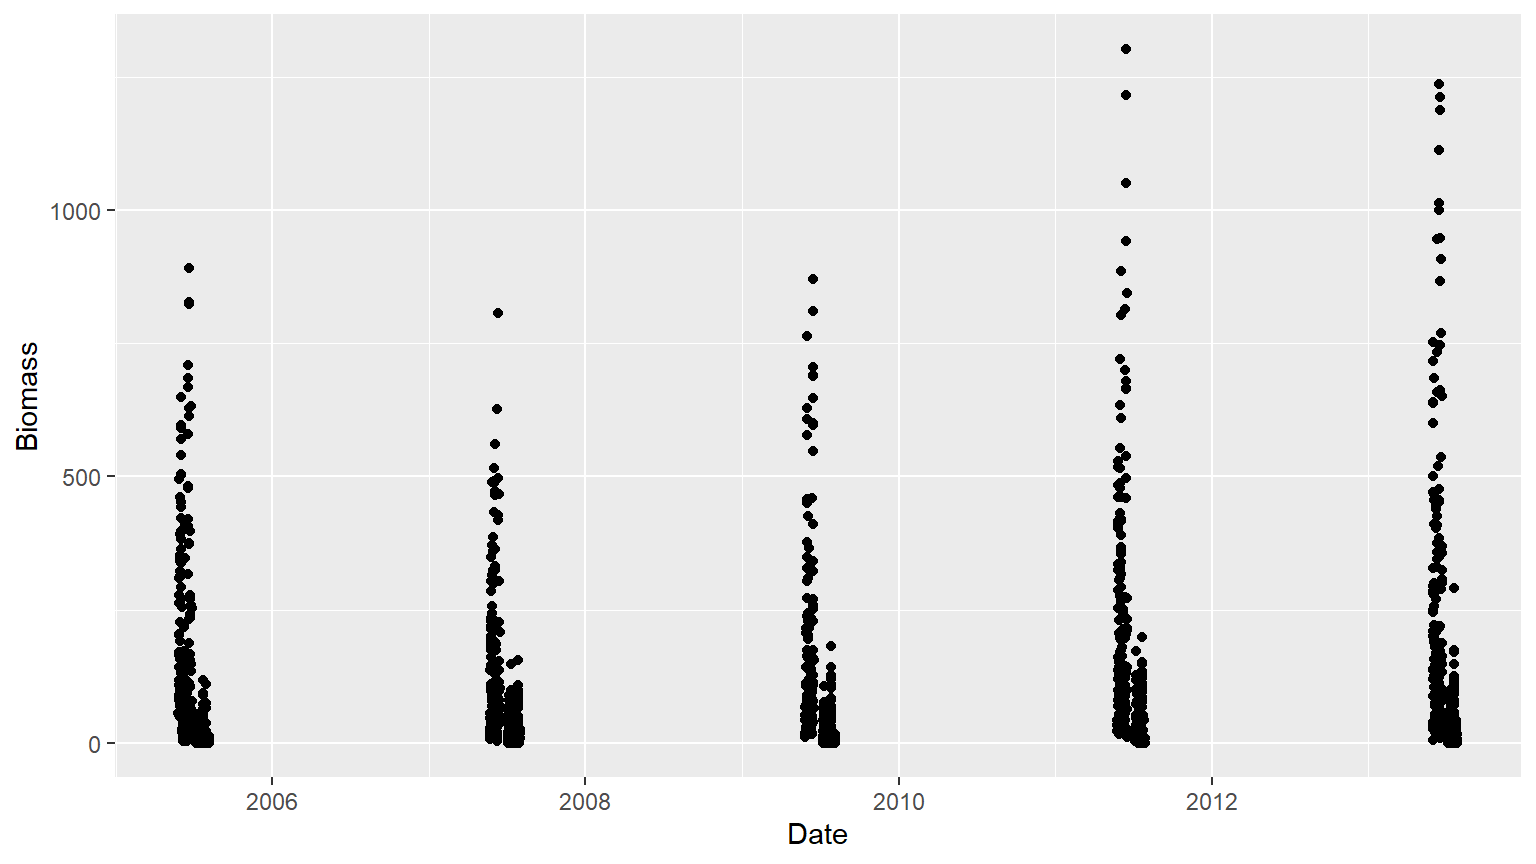
\includegraphics[width=.9\linewidth]{figure/sp_TSplot-1} 

}



\end{knitrout}
\end{frame}

\begin{frame}[fragile]{Time series}
\begin{knitrout}\footnotesize
\definecolor{shadecolor}{rgb}{0.969, 0.969, 0.969}\color{fgcolor}\begin{kframe}
\begin{alltt}
\hlstd{TSplot_year} \hlkwb{<-} \hlkwd{ggplot}\hlstd{(}\hlkwc{data}\hlstd{=df_data,} \hlkwd{aes}\hlstd{(}\hlkwc{x}\hlstd{=Year,} \hlkwc{y}\hlstd{=Biomass))} \hlopt{+}
  \hlkwd{geom_point}\hlstd{()}
\hlkwd{print}\hlstd{(TSplot_year)}
\end{alltt}
\end{kframe}

{\centering 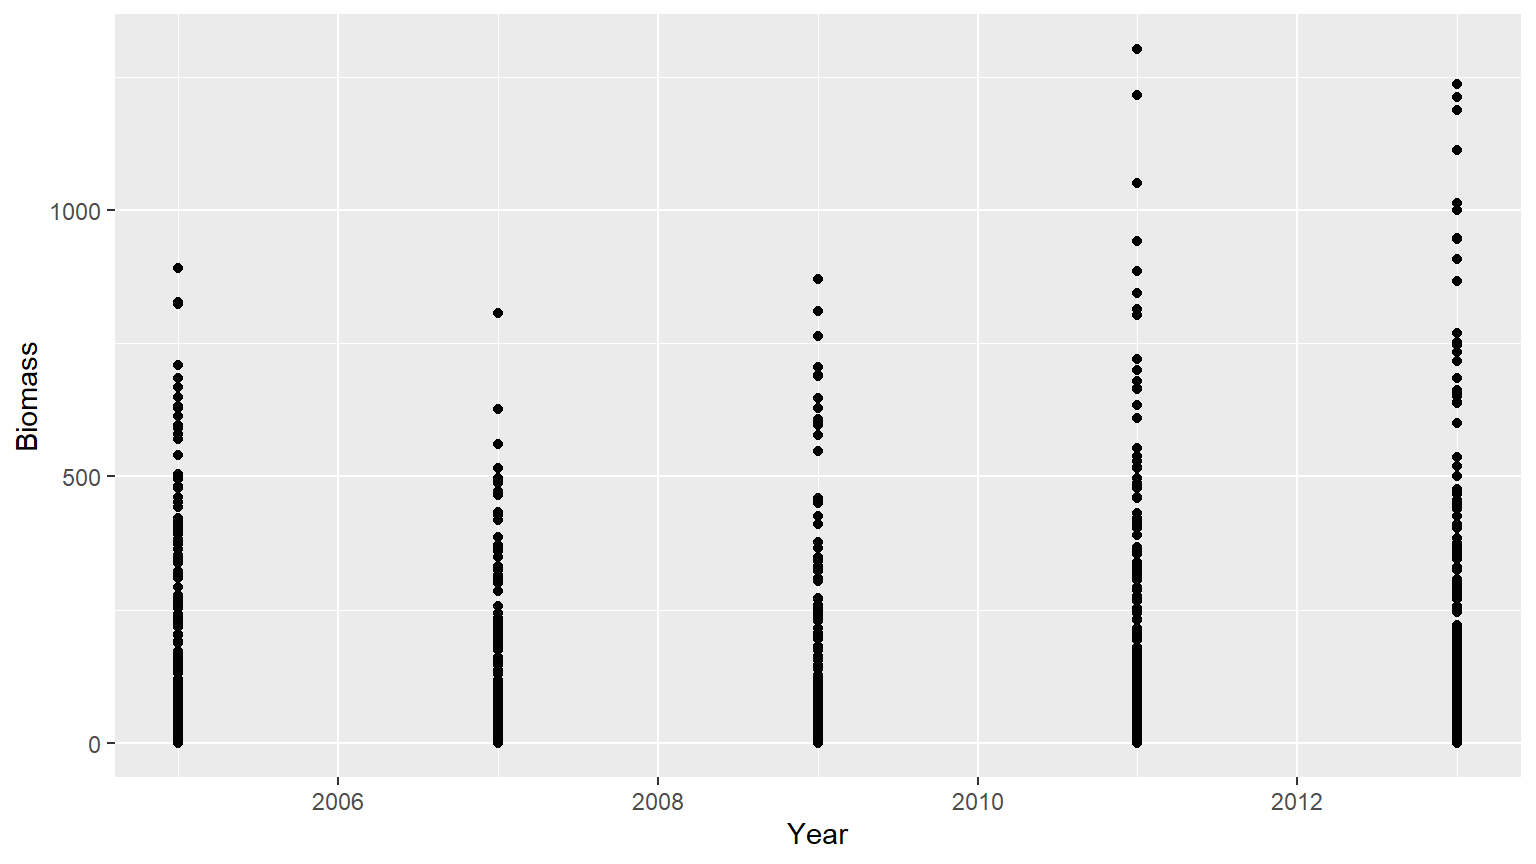
\includegraphics[width=.9\linewidth]{figure/sp_TSplot_year-1} 

}



\end{knitrout}
\end{frame}

\subsection{Summarize}
\begin{frame}[fragile]{Time series: summarize}
Summarize the data with the mean, median and quantiles for easy plotting.
The ddply function from the plyr R package provides an easy way to summarize the data.
\begin{knitrout}\footnotesize
\definecolor{shadecolor}{rgb}{0.969, 0.969, 0.969}\color{fgcolor}\begin{kframe}
\begin{alltt}
\hlstd{df_summary} \hlkwb{<-} \hlkwd{ddply}\hlstd{(df_data,} \hlkwd{c}\hlstd{(}\hlstr{'Year'}\hlstd{), summarise,}
                    \hlkwc{B_mean}\hlstd{=}\hlkwd{mean}\hlstd{(Biomass),}
                    \hlkwc{B_median}\hlstd{=}\hlkwd{median}\hlstd{(Biomass),}
                    \hlkwc{B_sd}\hlstd{=}\hlkwd{sd}\hlstd{(Biomass),}
                    \hlkwc{B_q025}\hlstd{=}\hlkwd{quantile}\hlstd{(Biomass,} \hlkwc{probs} \hlstd{=} \hlnum{0.025}\hlstd{),}
                    \hlkwc{B_q05}\hlstd{=}\hlkwd{quantile}\hlstd{(Biomass,} \hlkwc{probs} \hlstd{=} \hlnum{0.05}\hlstd{),}
                    \hlkwc{B_q10}\hlstd{=}\hlkwd{quantile}\hlstd{(Biomass,} \hlkwc{probs} \hlstd{=} \hlnum{0.10}\hlstd{),}
                    \hlkwc{B_q50}\hlstd{=}\hlkwd{quantile}\hlstd{(Biomass,} \hlkwc{probs} \hlstd{=} \hlnum{0.50}\hlstd{),}
                    \hlkwc{B_q90}\hlstd{=}\hlkwd{quantile}\hlstd{(Biomass,} \hlkwc{probs} \hlstd{=} \hlnum{0.90}\hlstd{),}
                    \hlkwc{B_q95}\hlstd{=}\hlkwd{quantile}\hlstd{(Biomass,} \hlkwc{probs} \hlstd{=} \hlnum{0.95}\hlstd{),}
                    \hlkwc{B_q975}\hlstd{=}\hlkwd{quantile}\hlstd{(Biomass,} \hlkwc{probs} \hlstd{=} \hlnum{0.975}\hlstd{))}
\end{alltt}
\end{kframe}
\end{knitrout}
\end{frame}

\begin{frame}[fragile]{Time series: summarize}
Summarize the data with the mean, median and quantiles for easy plotting.
The ddply function from the plyr R package provides an easy way to summarize the data.
\begin{knitrout}\footnotesize
\definecolor{shadecolor}{rgb}{0.969, 0.969, 0.969}\color{fgcolor}\begin{kframe}
\begin{alltt}
\hlkwd{str}\hlstd{(df_summary)}
\end{alltt}
\begin{verbatim}
## 'data.frame':	5 obs. of  11 variables:
##  $ Year    : int  2005 2007 2009 2011 2013
##  $ B_mean  : num  58.1 34.7 88.8 99.4 178.3
##  $ B_median: num  19.6 11.7 36.8 36.2 56.6
##  $ B_sd    : num  94.8 59.1 145.7 161.6 291.7
##  $ B_q025  : num  0 0 0 0 0
##  $ B_q05   : num  0 0 0 0 1.88
##  $ B_q10   : num  0 0 2.44 1.93 3.87
##  $ B_q50   : num  19.6 11.7 36.8 36.2 56.6
##  $ B_q90   : num  199 107 243 291 532
##  $ B_q95   : num  265 177 406 432 834
##  $ B_q975  : num  332 215 613 572 1112
\end{verbatim}
\end{kframe}
\end{knitrout}
\end{frame}


\subsection{Error bars}

\begin{frame}[fragile]{Time series with error bars}
\begin{knitrout}\footnotesize
\definecolor{shadecolor}{rgb}{0.969, 0.969, 0.969}\color{fgcolor}\begin{kframe}
\begin{alltt}
\hlstd{TSplot_i95} \hlkwb{<-} \hlkwd{ggplot}\hlstd{(}\hlkwc{data}\hlstd{=df_summary,} \hlkwd{aes}\hlstd{(}\hlkwc{x}\hlstd{=Year,} \hlkwc{y}\hlstd{=B_mean))} \hlopt{+}
  \hlkwd{geom_point}\hlstd{()}
\hlkwd{print}\hlstd{(TSplot_i95)}
\end{alltt}
\end{kframe}

{\centering 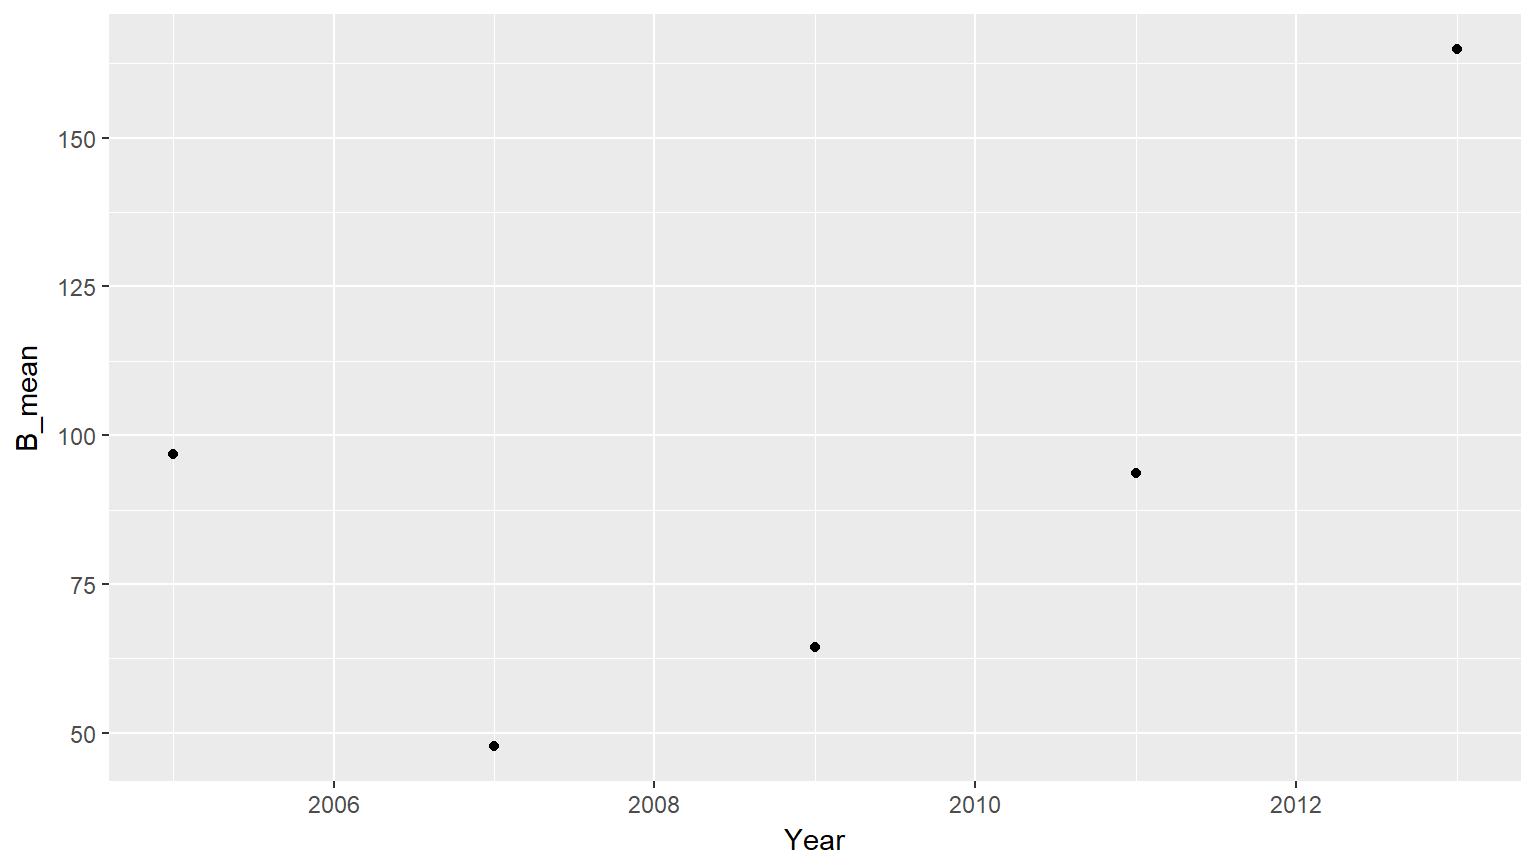
\includegraphics[width=.9\linewidth]{figure/sp_TSplot_i95a-1} 

}



\end{knitrout}
\end{frame}

\begin{frame}[fragile]{Time series with error bars}
\begin{knitrout}\footnotesize
\definecolor{shadecolor}{rgb}{0.969, 0.969, 0.969}\color{fgcolor}\begin{kframe}
\begin{alltt}
\hlstd{TSplot_i95} \hlkwb{<-} \hlstd{TSplot_i95} \hlopt{+}
  \hlkwd{geom_pointrange}\hlstd{(}\hlkwd{aes}\hlstd{(}\hlkwc{ymin} \hlstd{= B_q025,} \hlkwc{ymax} \hlstd{= B_q975))}
\hlkwd{print}\hlstd{(TSplot_i95)}
\end{alltt}
\end{kframe}

{\centering 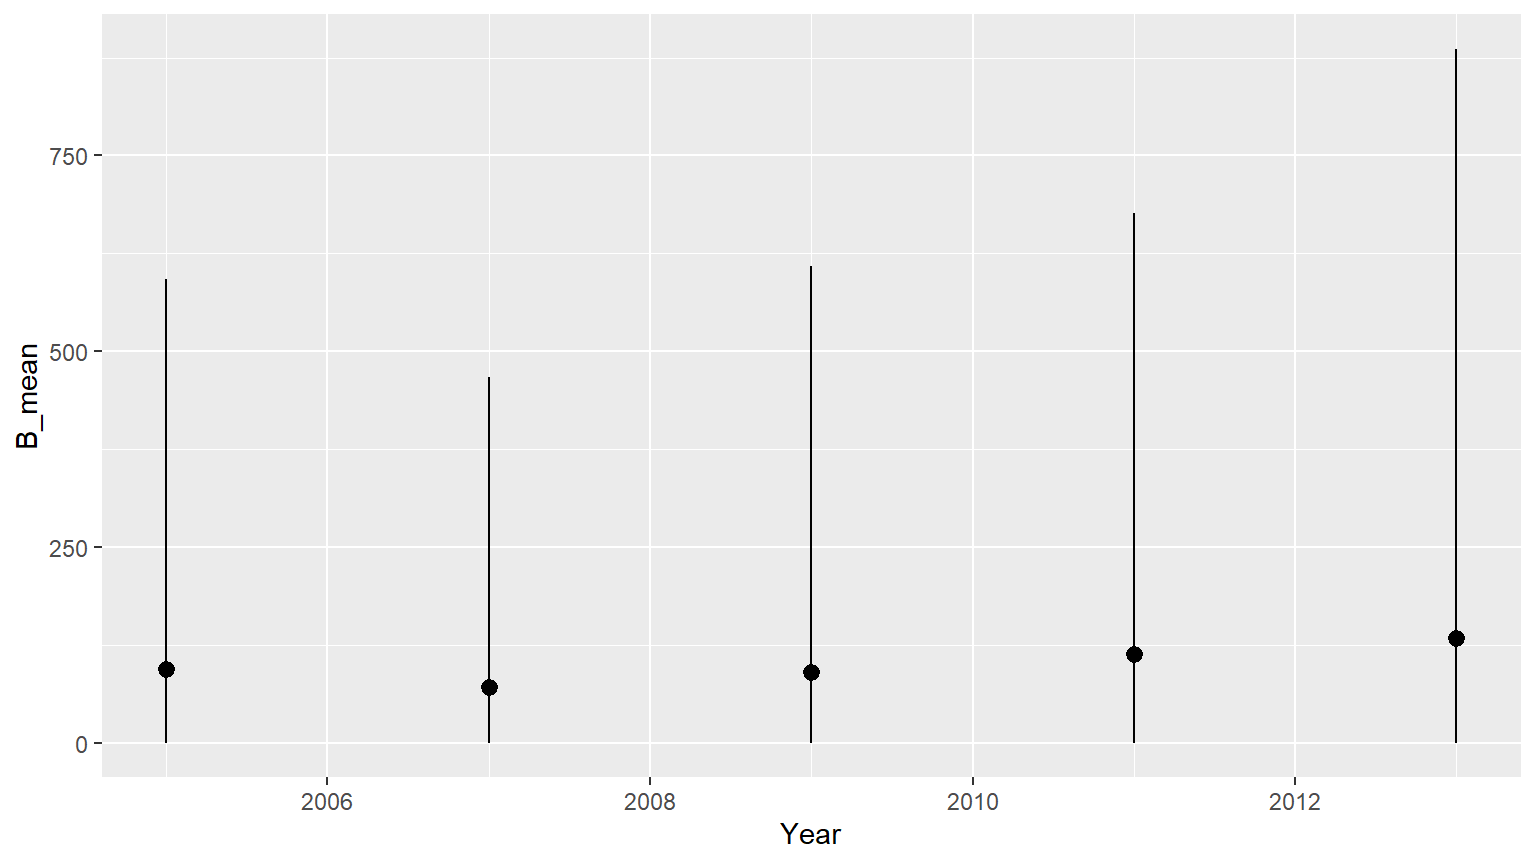
\includegraphics[width=.9\linewidth]{figure/sp_TSplot_i95b-1} 

}



\end{knitrout}
\end{frame}


\begin{frame}[fragile]{Time series with error bars}
\begin{knitrout}\footnotesize
\definecolor{shadecolor}{rgb}{0.969, 0.969, 0.969}\color{fgcolor}\begin{kframe}
\begin{alltt}
\hlstd{TSplot_errori95} \hlkwb{<-} \hlkwd{ggplot}\hlstd{(}\hlkwc{data}\hlstd{=df_summary,} \hlkwd{aes}\hlstd{(}\hlkwc{x}\hlstd{=Year,} \hlkwc{y}\hlstd{=B_mean))} \hlopt{+}
  \hlkwd{geom_line}\hlstd{()} \hlopt{+}
  \hlkwd{geom_errorbar}\hlstd{(}\hlkwd{aes}\hlstd{(}\hlkwc{ymin} \hlstd{= B_q025,} \hlkwc{ymax} \hlstd{= B_q975),} \hlkwc{width} \hlstd{=} \hlnum{0.2}\hlstd{)}
\hlkwd{print}\hlstd{(TSplot_errori95)}
\end{alltt}
\end{kframe}

{\centering 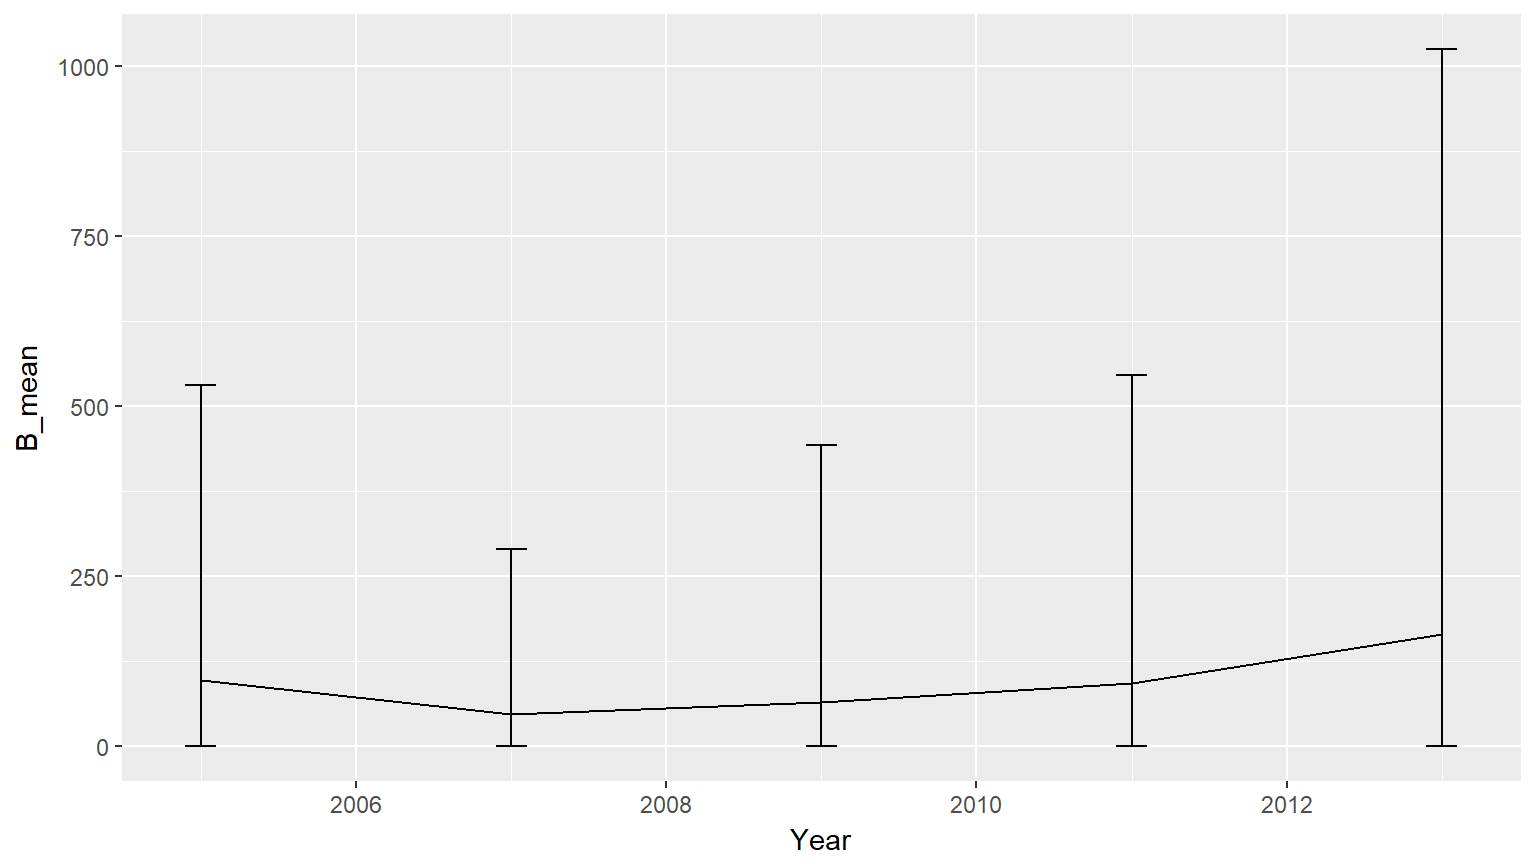
\includegraphics[width=.9\linewidth]{figure/sp_TSplot_errori95-1} 

}



\end{knitrout}
\end{frame}



\begin{frame}[fragile]{Time series with error bars: Improvement}
\begin{knitrout}\footnotesize
\definecolor{shadecolor}{rgb}{0.969, 0.969, 0.969}\color{fgcolor}\begin{kframe}
\begin{alltt}
\hlstd{TSplot_i95} \hlkwb{<-} \hlkwd{ggplot}\hlstd{(}\hlkwc{data}\hlstd{=df_summary,} \hlkwd{aes}\hlstd{(}\hlkwc{x}\hlstd{=Year,} \hlkwc{y}\hlstd{=B_mean))} \hlopt{+}
  \hlkwd{geom_point}\hlstd{()} \hlopt{+}
  \hlkwd{geom_pointrange}\hlstd{(}\hlkwd{aes}\hlstd{(}\hlkwc{ymin} \hlstd{= B_q025,} \hlkwc{ymax} \hlstd{= B_q975))}
\hlkwd{print}\hlstd{(TSplot_i95)}
\end{alltt}
\end{kframe}

{\centering 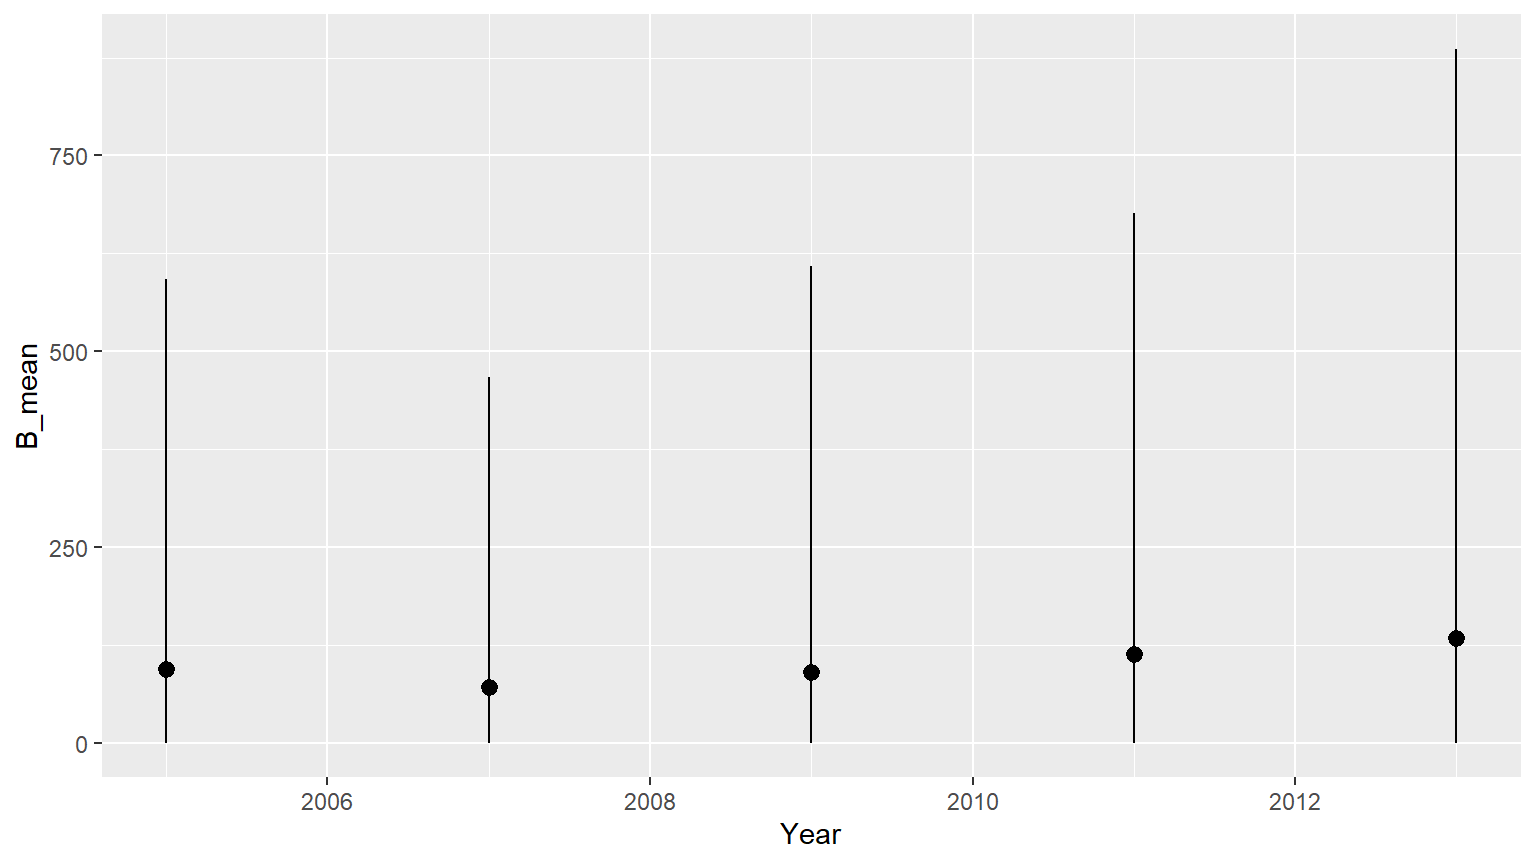
\includegraphics[width=.9\linewidth]{figure/sp_TSplot_i95_bis-1} 

}



\end{knitrout}
\end{frame}

\begin{frame}[fragile]{Time series with error bars: Improvement}
\begin{knitrout}\footnotesize
\definecolor{shadecolor}{rgb}{0.969, 0.969, 0.969}\color{fgcolor}\begin{kframe}
\begin{alltt}
\hlstd{TSplot_i95} \hlkwb{<-} \hlkwd{ggplot}\hlstd{(}\hlkwc{data}\hlstd{=df_summary,} \hlkwd{aes}\hlstd{(}\hlkwc{x}\hlstd{=Year,} \hlkwc{y}\hlstd{=B_mean))} \hlopt{+}
  \hlkwd{geom_point}\hlstd{()} \hlopt{+} \hlkwd{geom_pointrange}\hlstd{(}\hlkwd{aes}\hlstd{(}\hlkwc{ymin} \hlstd{= B_q025,} \hlkwc{ymax} \hlstd{= B_q975))} \hlopt{+}
  \hlkwd{ylab}\hlstd{(}\hlstr{'Biomass'}\hlstd{)} \hlopt{+}
  \hlkwd{scale_x_continuous}\hlstd{(}\hlkwc{name} \hlstd{=} \hlstr{'Year'}\hlstd{,} \hlkwc{breaks} \hlstd{=} \hlkwd{seq}\hlstd{(}\hlnum{2005}\hlstd{,} \hlnum{2013}\hlstd{,} \hlkwc{by} \hlstd{=} \hlnum{1}\hlstd{))}
\hlkwd{print}\hlstd{(TSplot_i95)}
\end{alltt}
\end{kframe}

{\centering 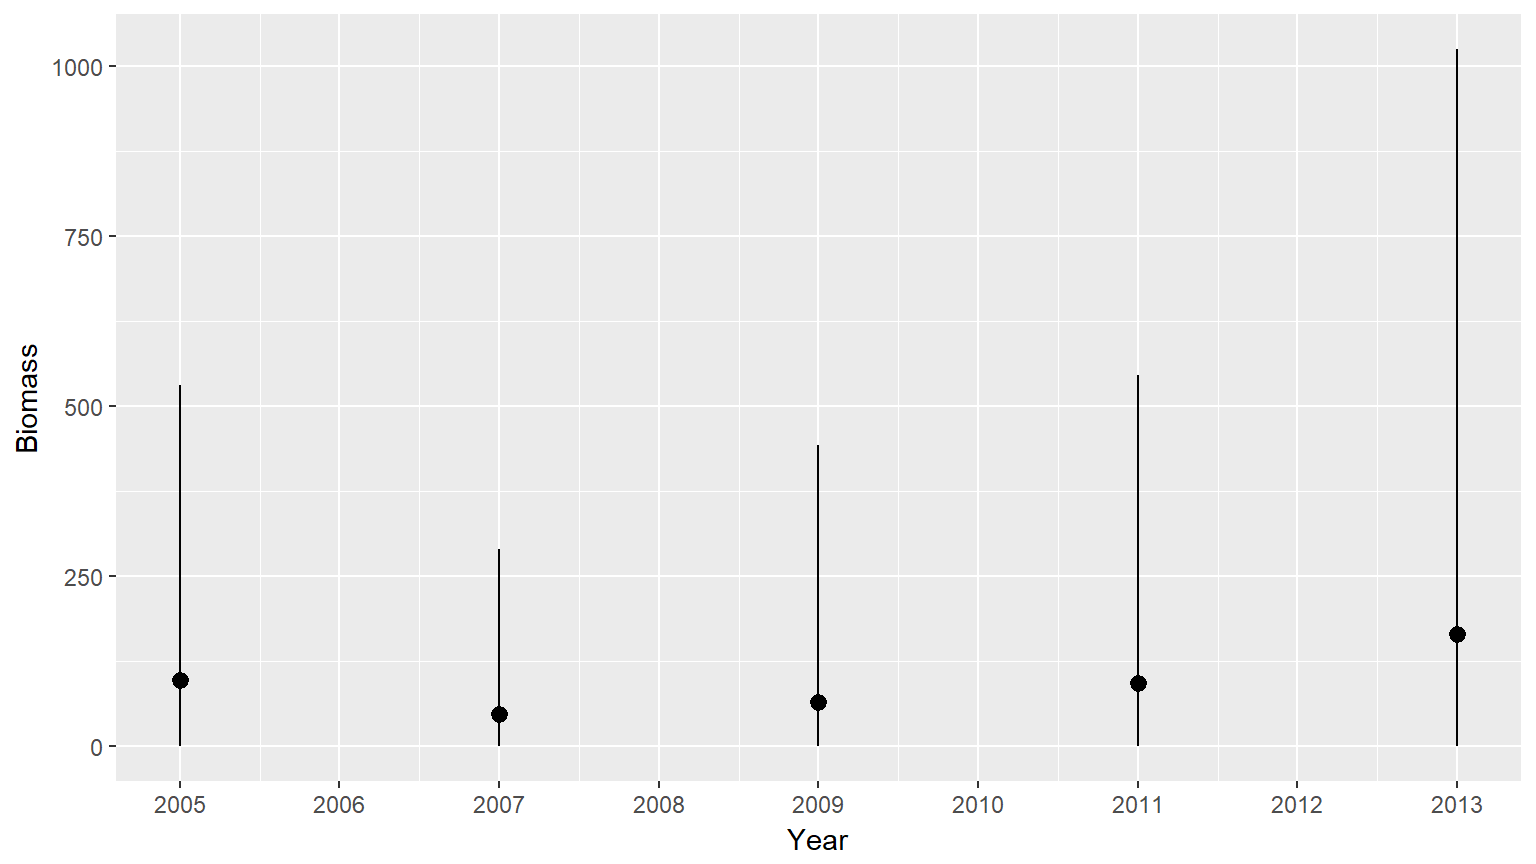
\includegraphics[width=.9\linewidth]{figure/sp_TSplot_i95_imp-1} 

}



\end{knitrout}
\end{frame}

\begin{frame}[fragile]{Time series with \lstinline{geom_ribbon}}
\begin{knitrout}\footnotesize
\definecolor{shadecolor}{rgb}{0.969, 0.969, 0.969}\color{fgcolor}\begin{kframe}
\begin{alltt}
\hlstd{TSplot_ri95} \hlkwb{<-} \hlkwd{ggplot}\hlstd{(}\hlkwc{data}\hlstd{=df_summary,} \hlkwd{aes}\hlstd{(}\hlkwc{x}\hlstd{=Year,} \hlkwc{y}\hlstd{=B_mean))} \hlopt{+}
  \hlkwd{geom_ribbon}\hlstd{(}\hlkwd{aes}\hlstd{(}\hlkwc{ymin} \hlstd{= B_q025,} \hlkwc{ymax} \hlstd{= B_q975),} \hlkwc{fill} \hlstd{=} \hlstr{"blue"}\hlstd{,} \hlkwc{alpha}\hlstd{=}\hlnum{0.2}\hlstd{)} \hlopt{+}
  \hlkwd{geom_point}\hlstd{()} \hlopt{+} \hlkwd{geom_line}\hlstd{()} \hlopt{+} \hlkwd{ylab}\hlstd{(}\hlstr{'Biomass'}\hlstd{)} \hlopt{+}
  \hlkwd{scale_x_continuous}\hlstd{(}\hlkwc{name} \hlstd{=} \hlstr{'Year'}\hlstd{,} \hlkwc{breaks} \hlstd{=} \hlkwd{seq}\hlstd{(}\hlnum{2005}\hlstd{,} \hlnum{2013}\hlstd{,} \hlkwc{by} \hlstd{=} \hlnum{1}\hlstd{))}
\hlkwd{print}\hlstd{(TSplot_ri95)}
\end{alltt}
\end{kframe}

{\centering 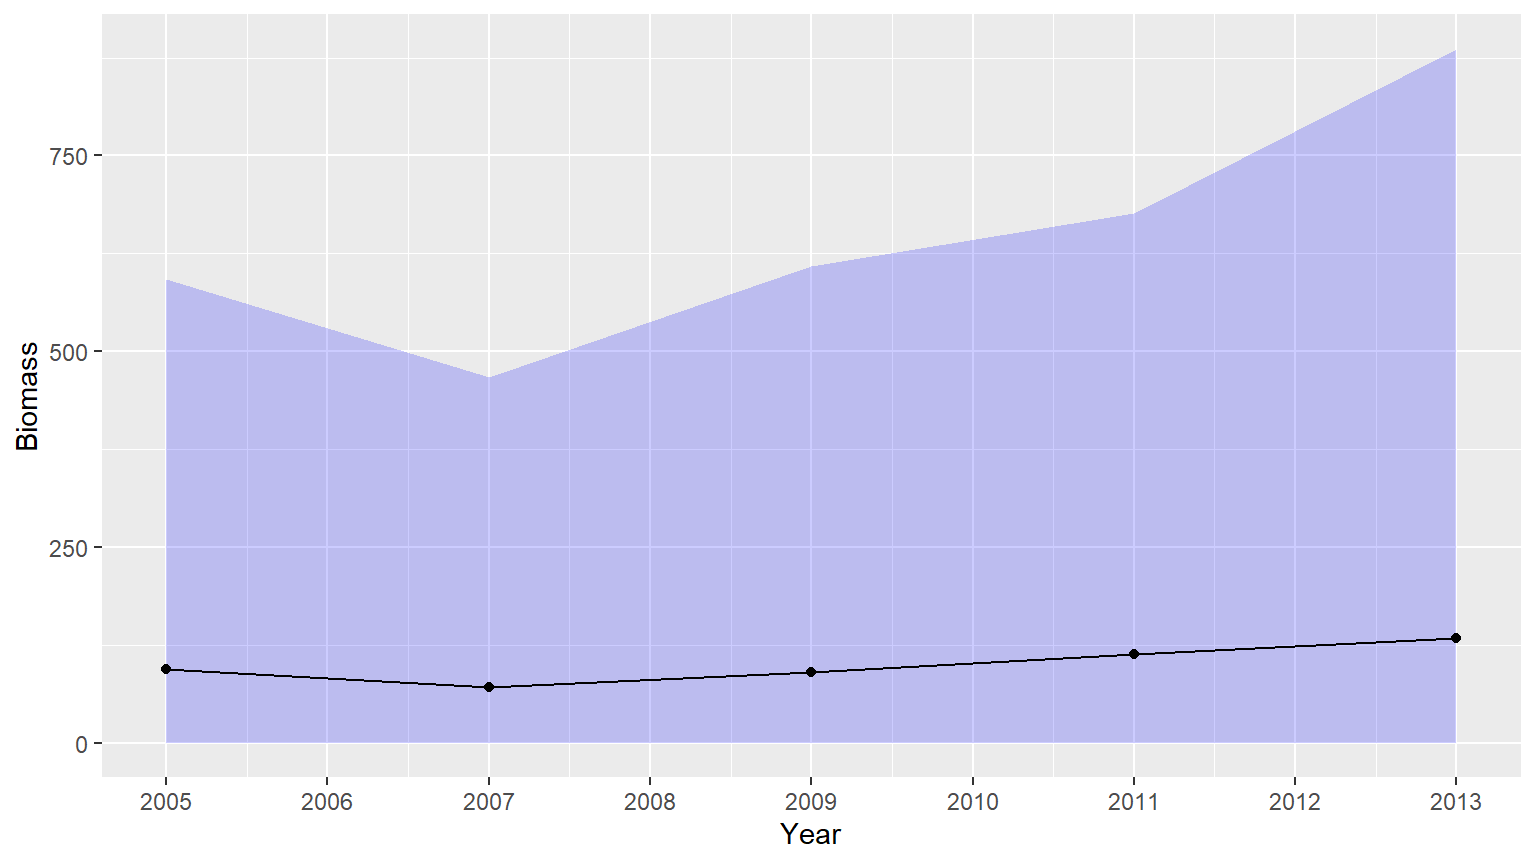
\includegraphics[width=.9\linewidth]{figure/sp_TSplot_ri95-1} 

}



\end{knitrout}
\end{frame}

%%% X-axis as a Date format

\begin{frame}[fragile]{Time series: x-axis as date}
\begin{knitrout}\footnotesize
\definecolor{shadecolor}{rgb}{0.969, 0.969, 0.969}\color{fgcolor}\begin{kframe}
\begin{alltt}
\hlstd{TSplot} \hlkwb{<-} \hlkwd{ggplot}\hlstd{(}\hlkwc{data}\hlstd{=df_data,} \hlkwd{aes}\hlstd{(}\hlkwc{x}\hlstd{=Date,} \hlkwc{y}\hlstd{=Biomass))} \hlopt{+}
  \hlkwd{geom_point}\hlstd{()} \hlopt{+}
  \hlkwd{ylab}\hlstd{(}\hlstr{'Biomass (kg)'}\hlstd{)}
\hlkwd{print}\hlstd{(TSplot)}
\end{alltt}
\end{kframe}

{\centering 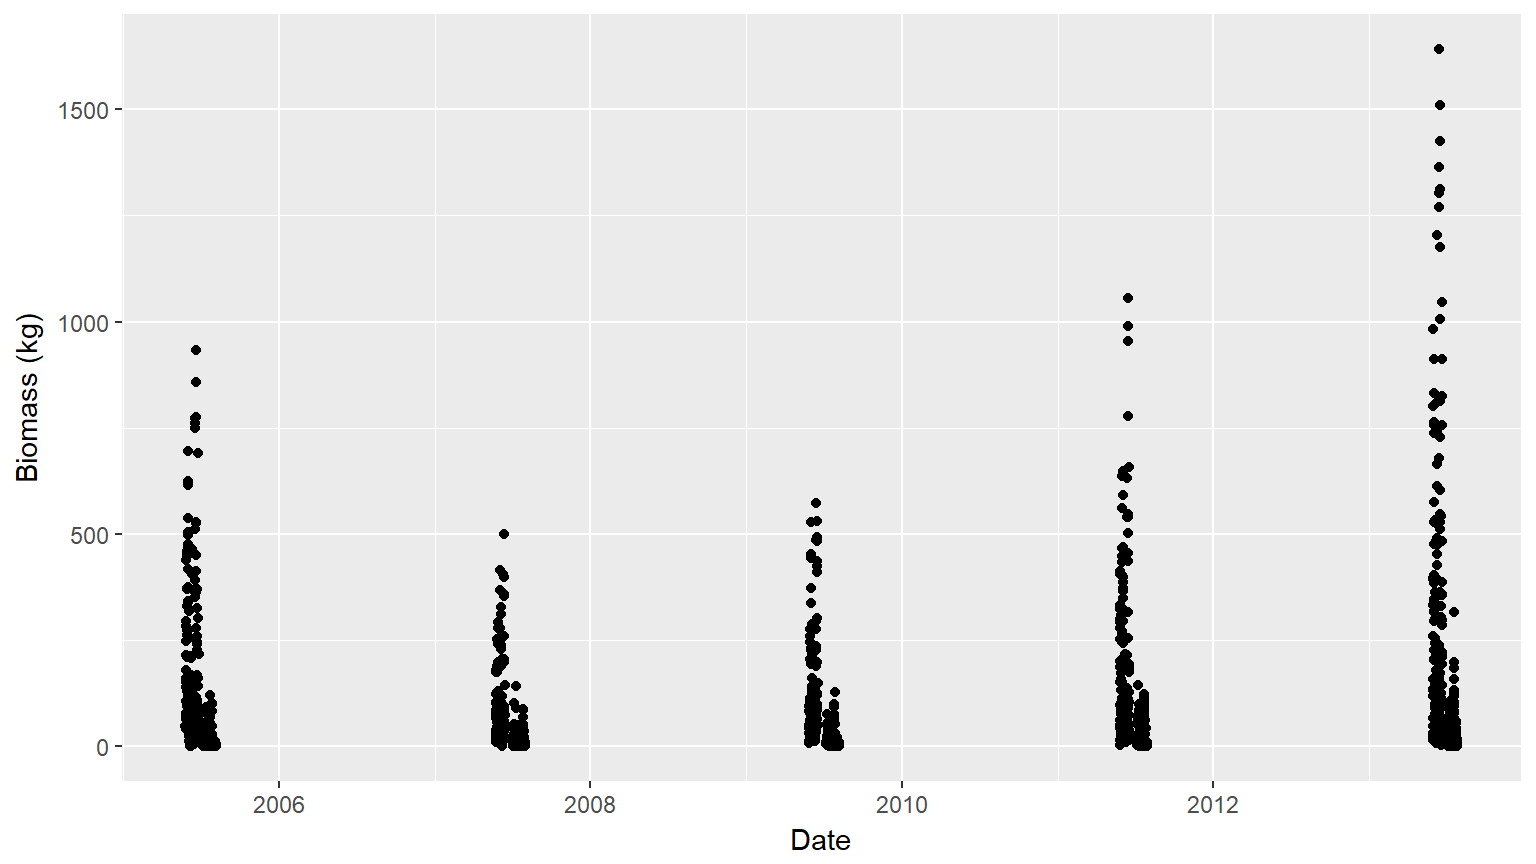
\includegraphics[width=.9\linewidth]{figure/TSplot_i95d1-1} 

}



\end{knitrout}
\end{frame}

\begin{frame}[fragile]{Time series: x-axis as date}
\begin{knitrout}\footnotesize
\definecolor{shadecolor}{rgb}{0.969, 0.969, 0.969}\color{fgcolor}\begin{kframe}
\begin{alltt}
\hlcom{# Months only}
\hlstd{TSplotm} \hlkwb{<-} \hlstd{TSplot} \hlopt{+}
  \hlkwd{scale_x_date}\hlstd{(}\hlkwc{labels} \hlstd{=} \hlkwd{date_format}\hlstd{(}\hlstr{"%y/%b"}\hlstd{),} \hlkwc{date_breaks}\hlstd{=}\hlstr{"1 year"}\hlstd{,}
               \hlkwc{date_minor_breaks} \hlstd{=} \hlstr{"1 month"}\hlstd{)} \hlopt{+}
  \hlkwd{theme}\hlstd{(}\hlkwc{axis.text.x} \hlstd{=} \hlkwd{element_text}\hlstd{(}\hlkwc{angle}\hlstd{=}\hlnum{45}\hlstd{))}
\hlkwd{print}\hlstd{(TSplotm)}
\end{alltt}
\end{kframe}

{\centering 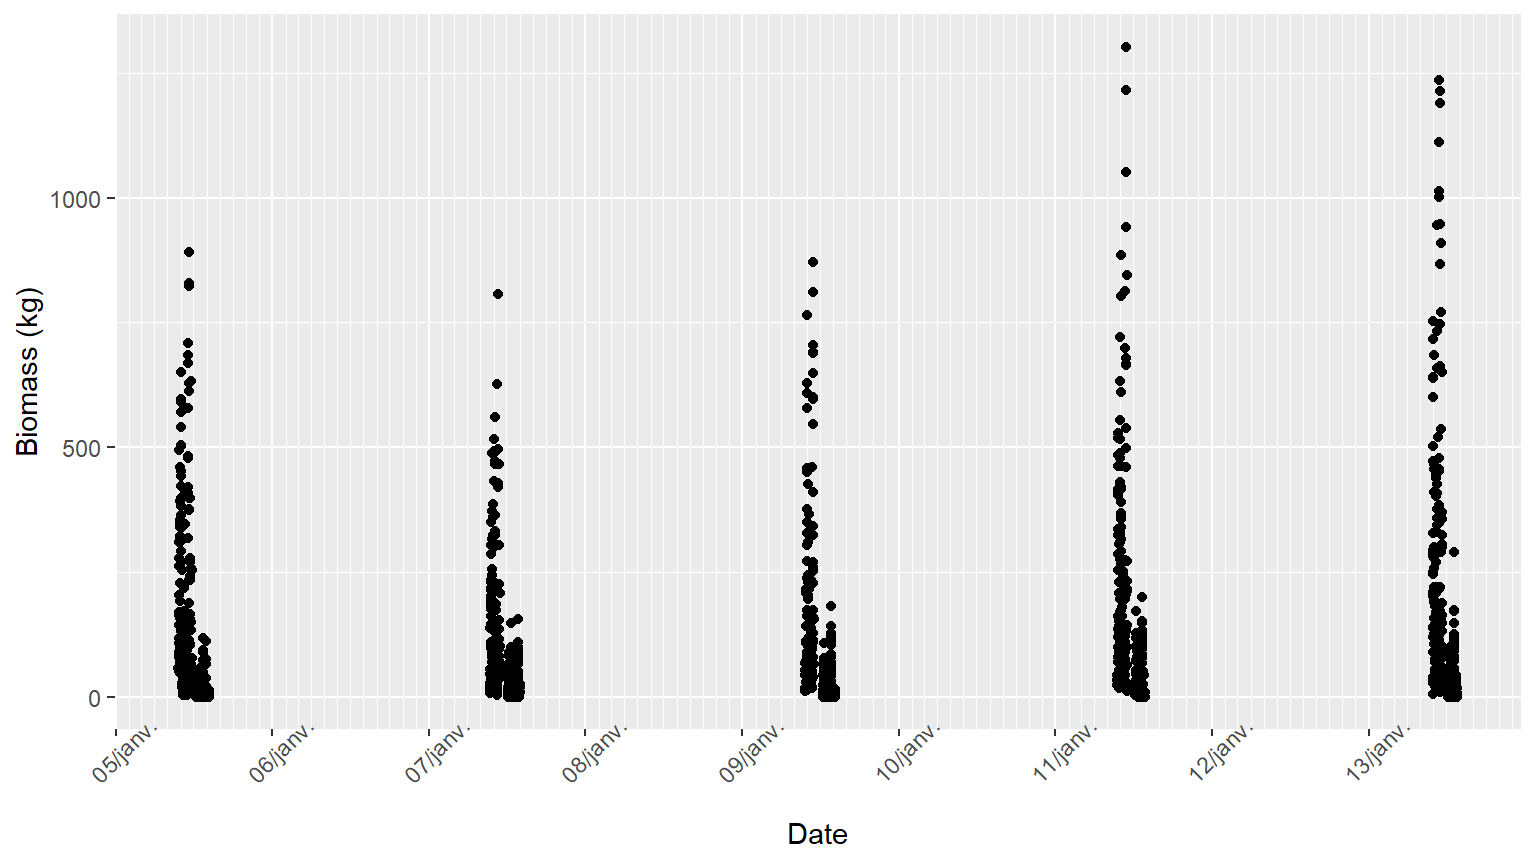
\includegraphics[width=.9\linewidth]{figure/TSplot_i95d4-1} 

}



\end{knitrout}
\end{frame}

\begin{frame}[fragile]{Time series: x-axis as date}
\begin{knitrout}\footnotesize
\definecolor{shadecolor}{rgb}{0.969, 0.969, 0.969}\color{fgcolor}\begin{kframe}
\begin{alltt}
\hlcom{# Format : Year/month}
\hlstd{TSplotym} \hlkwb{<-} \hlstd{TSplot} \hlopt{+}
  \hlkwd{scale_x_date}\hlstd{(}\hlkwc{labels} \hlstd{=} \hlkwd{date_format}\hlstd{(}\hlstr{"%Y/%m"}\hlstd{))}
\hlkwd{print}\hlstd{(TSplotym)}
\end{alltt}
\end{kframe}

{\centering 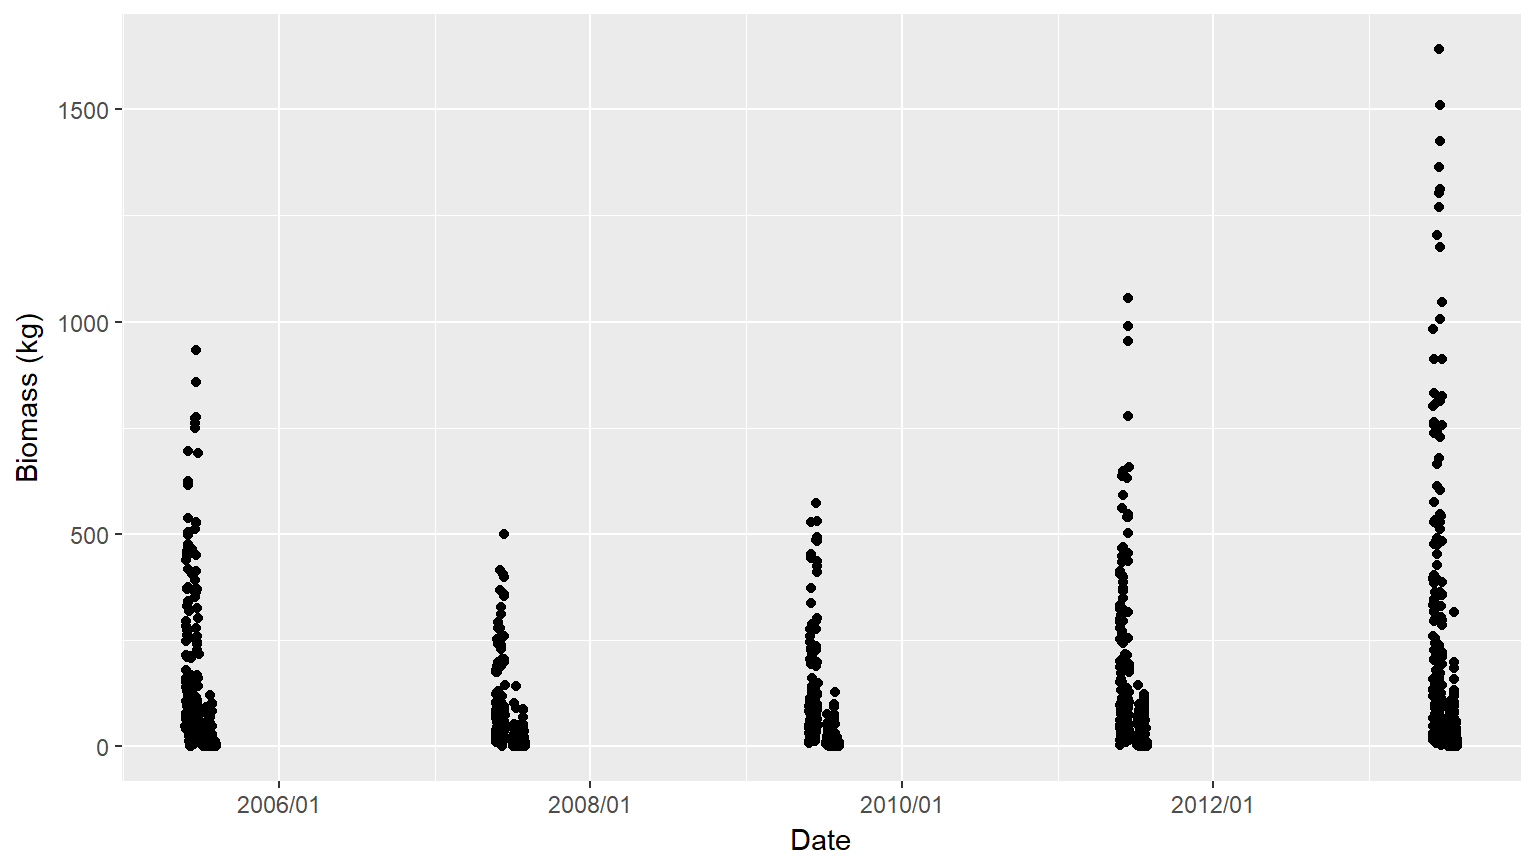
\includegraphics[width=.9\linewidth]{figure/TSplot_i95d3-1} 

}



\end{knitrout}
\end{frame}

\begin{frame}[fragile]{Time series: x-axis as date}
\begin{knitrout}\footnotesize
\definecolor{shadecolor}{rgb}{0.969, 0.969, 0.969}\color{fgcolor}\begin{kframe}
\begin{alltt}
\hlcom{# Format : Year/month/day}
\hlstd{lmin} \hlkwb{<-} \hlkwd{as.Date}\hlstd{(}\hlstr{"2011-1-1"}\hlstd{); lmax} \hlkwb{<-} \hlkwd{max}\hlstd{(df_data}\hlopt{$}\hlstd{Date)}
\hlstd{TSplotymdl} \hlkwb{<-} \hlstd{TSplot} \hlopt{+}
  \hlkwd{scale_x_date}\hlstd{(}\hlkwc{labels} \hlstd{=} \hlkwd{date_format}\hlstd{(}\hlstr{"%y/%m/%d"}\hlstd{),} \hlkwc{limits} \hlstd{=} \hlkwd{c}\hlstd{(lmin, lmax))}
\hlkwd{print}\hlstd{(TSplotymdl)}
\end{alltt}
\end{kframe}

{\centering 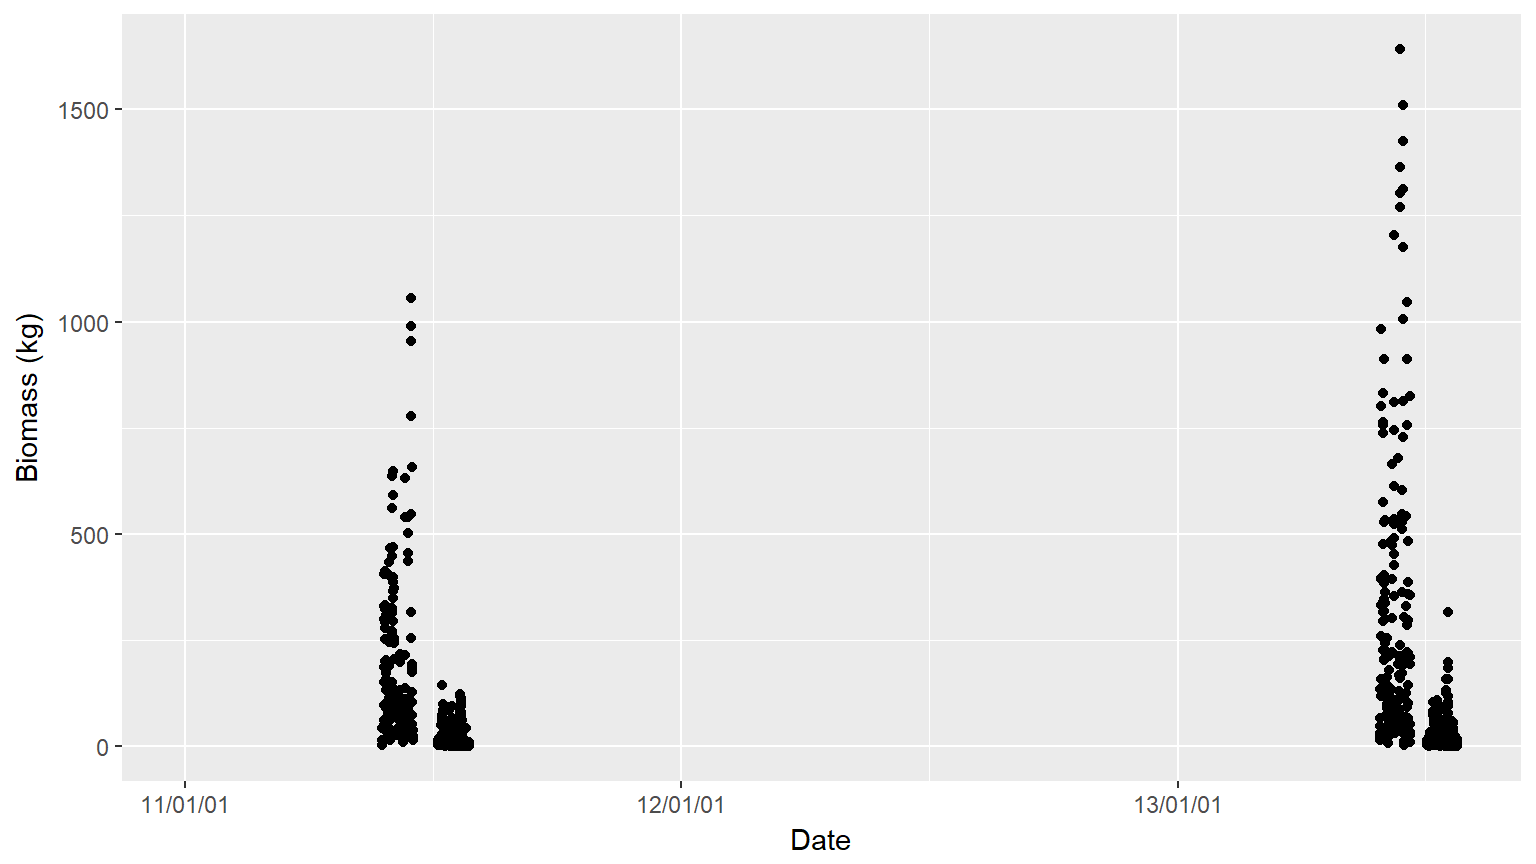
\includegraphics[width=.9\linewidth]{figure/TSplot_i95d2-1} 

}



\end{knitrout}
\end{frame}

%%%%%%%%%%%%%%%%%%%%%%%%%%%%%%%%%%%%%%%%%%%%%%%%%%%%%%%%%%%%%%%%%%%%%%%%%%%%%%%%
%%% Boxplot
%%%%%%%%%%%%%%%%%%%%%%%%%%%%%%%%%%%%%%%%%%%%%%%%%%%%%%%%%%%%%%%%%%%%%%%%%%%%%%%%
\subsection{Boxplots}
\begin{frame}[fragile]{Boxplot}
\begin{knitrout}\footnotesize
\definecolor{shadecolor}{rgb}{0.969, 0.969, 0.969}\color{fgcolor}\begin{kframe}
\begin{alltt}
\hlstd{boxplot_TS} \hlkwb{<-} \hlkwd{ggplot}\hlstd{(}\hlkwc{data}\hlstd{=df_data,} \hlkwd{aes}\hlstd{(}\hlkwc{x}\hlstd{=Year,} \hlkwc{y}\hlstd{=Biomass))} \hlopt{+}
  \hlkwd{geom_boxplot}\hlstd{()}
\hlkwd{print}\hlstd{(boxplot_TS)}
\end{alltt}


{\ttfamily\noindent\color{warningcolor}{\#\# Warning: Continuous x aesthetic -- did you forget aes(group=...)?}}\end{kframe}

{\centering 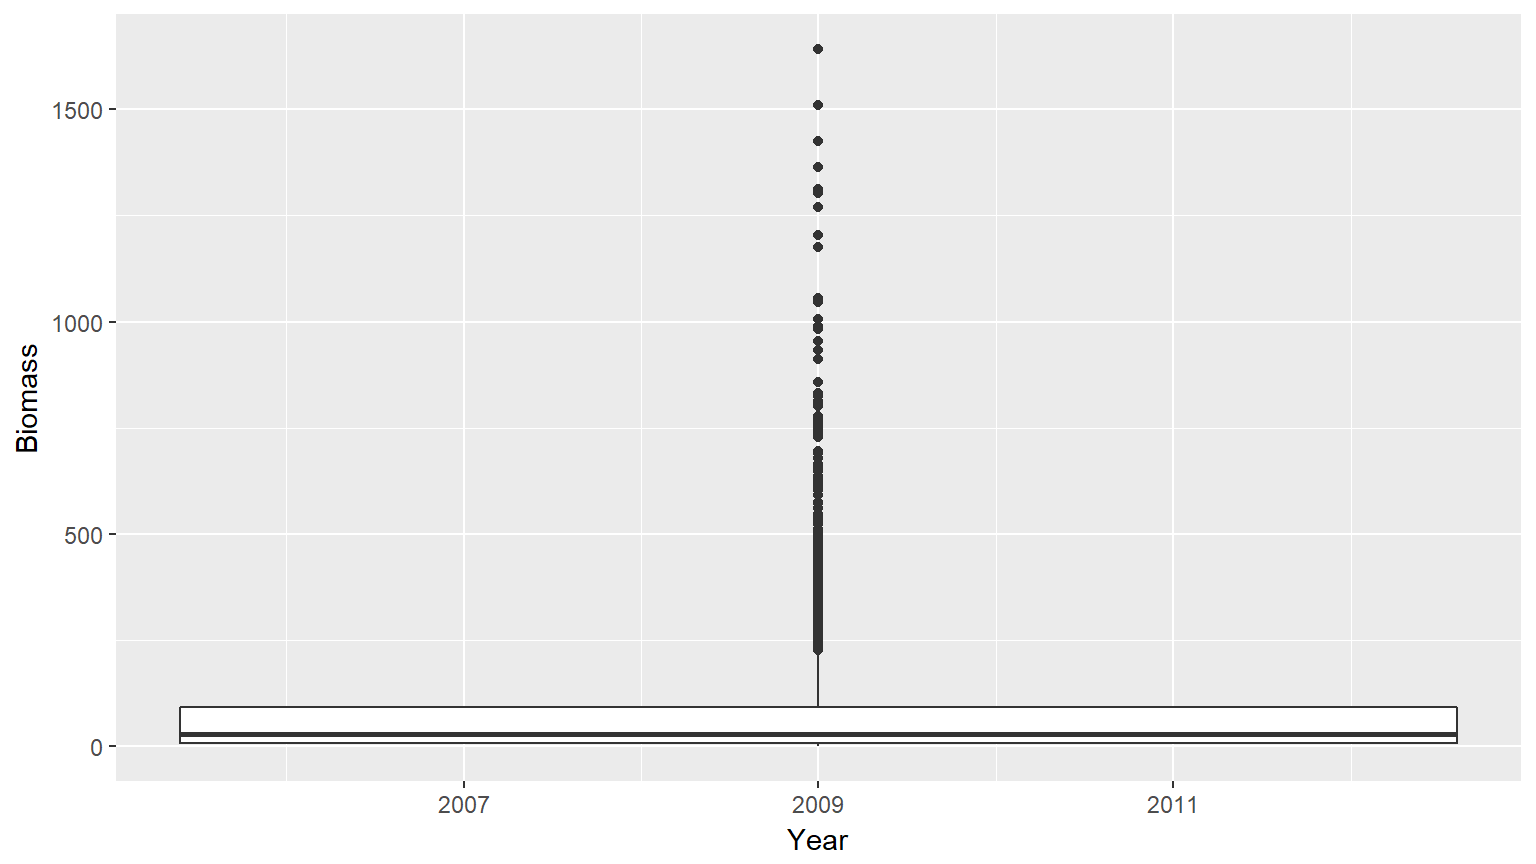
\includegraphics[width=.9\linewidth]{figure/boxplot_TS-1} 

}



\end{knitrout}
\end{frame}


\begin{frame}[fragile]{Boxplot with Year as a factor}
\begin{knitrout}\footnotesize
\definecolor{shadecolor}{rgb}{0.969, 0.969, 0.969}\color{fgcolor}\begin{kframe}
\begin{alltt}
\hlstd{boxplot_TSf} \hlkwb{<-} \hlkwd{ggplot}\hlstd{(}\hlkwc{data}\hlstd{=df_data,} \hlkwd{aes}\hlstd{(}\hlkwc{x}\hlstd{=}\hlkwd{factor}\hlstd{(Year),} \hlkwc{y}\hlstd{=Biomass))} \hlopt{+}
  \hlkwd{geom_boxplot}\hlstd{()}
\hlkwd{print}\hlstd{(boxplot_TSf)}
\end{alltt}
\end{kframe}

{\centering 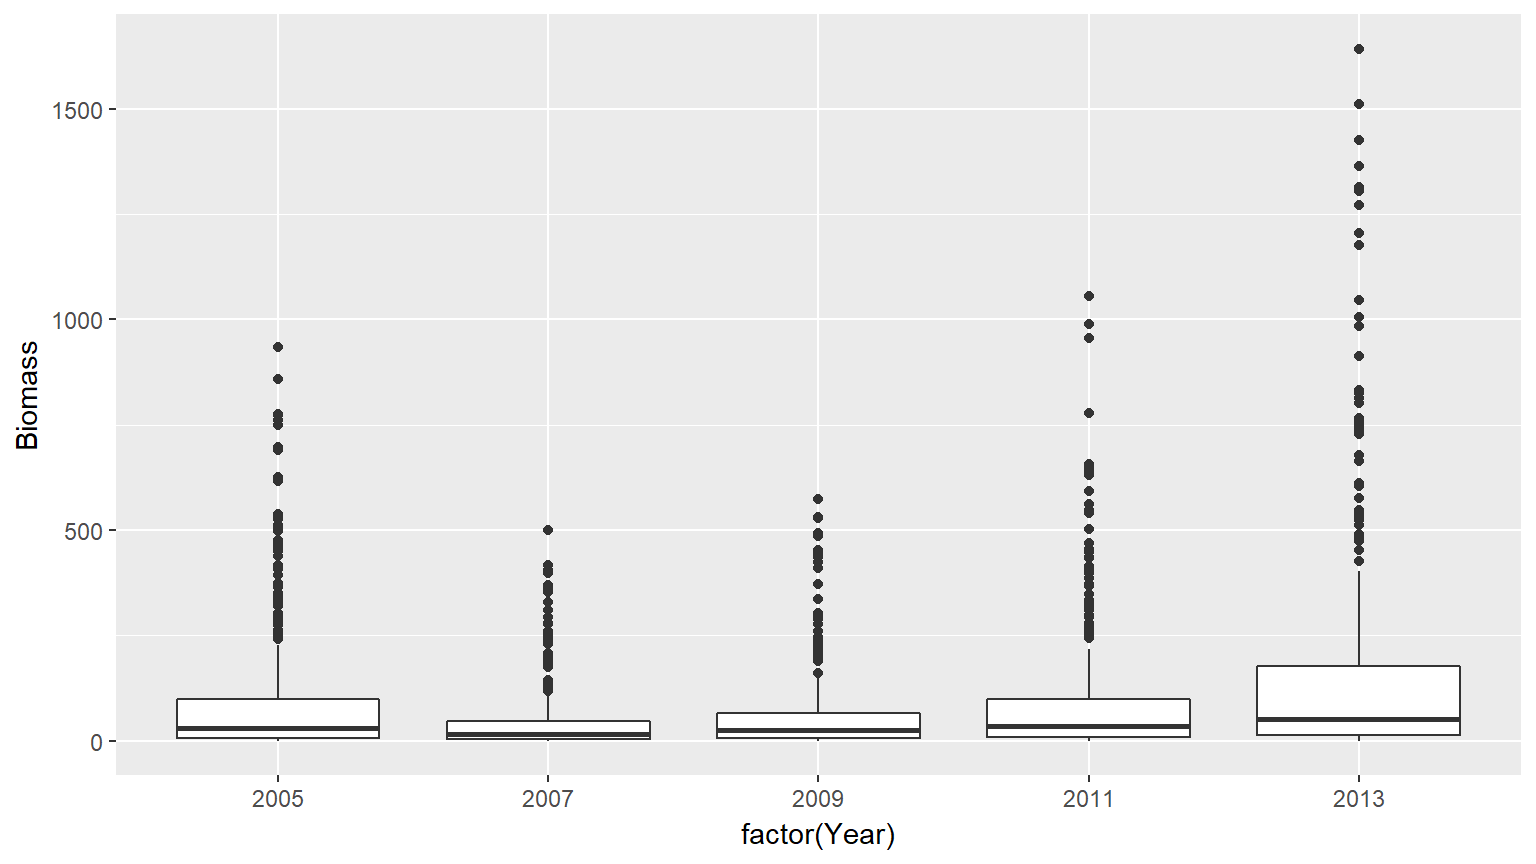
\includegraphics[width=.9\linewidth]{figure/boxplot_TSf-1} 

}



\end{knitrout}
\end{frame}

\begin{frame}[fragile]{Boxplot with Year and Area as a factor}
\begin{knitrout}\footnotesize
\definecolor{shadecolor}{rgb}{0.969, 0.969, 0.969}\color{fgcolor}\begin{kframe}
\begin{alltt}
\hlstd{boxplot_TS_AREA} \hlkwb{<-} \hlkwd{ggplot}\hlstd{(}\hlkwc{data}\hlstd{=df_data,} \hlkwd{aes}\hlstd{(}\hlkwc{x}\hlstd{=}\hlkwd{factor}\hlstd{(Year),} \hlkwc{y}\hlstd{=Biomass,}
                                            \hlkwc{colour}\hlstd{=AREA))} \hlopt{+}
  \hlkwd{geom_boxplot}\hlstd{()}
\hlkwd{print}\hlstd{(boxplot_TS_AREA)}
\end{alltt}
\end{kframe}

{\centering 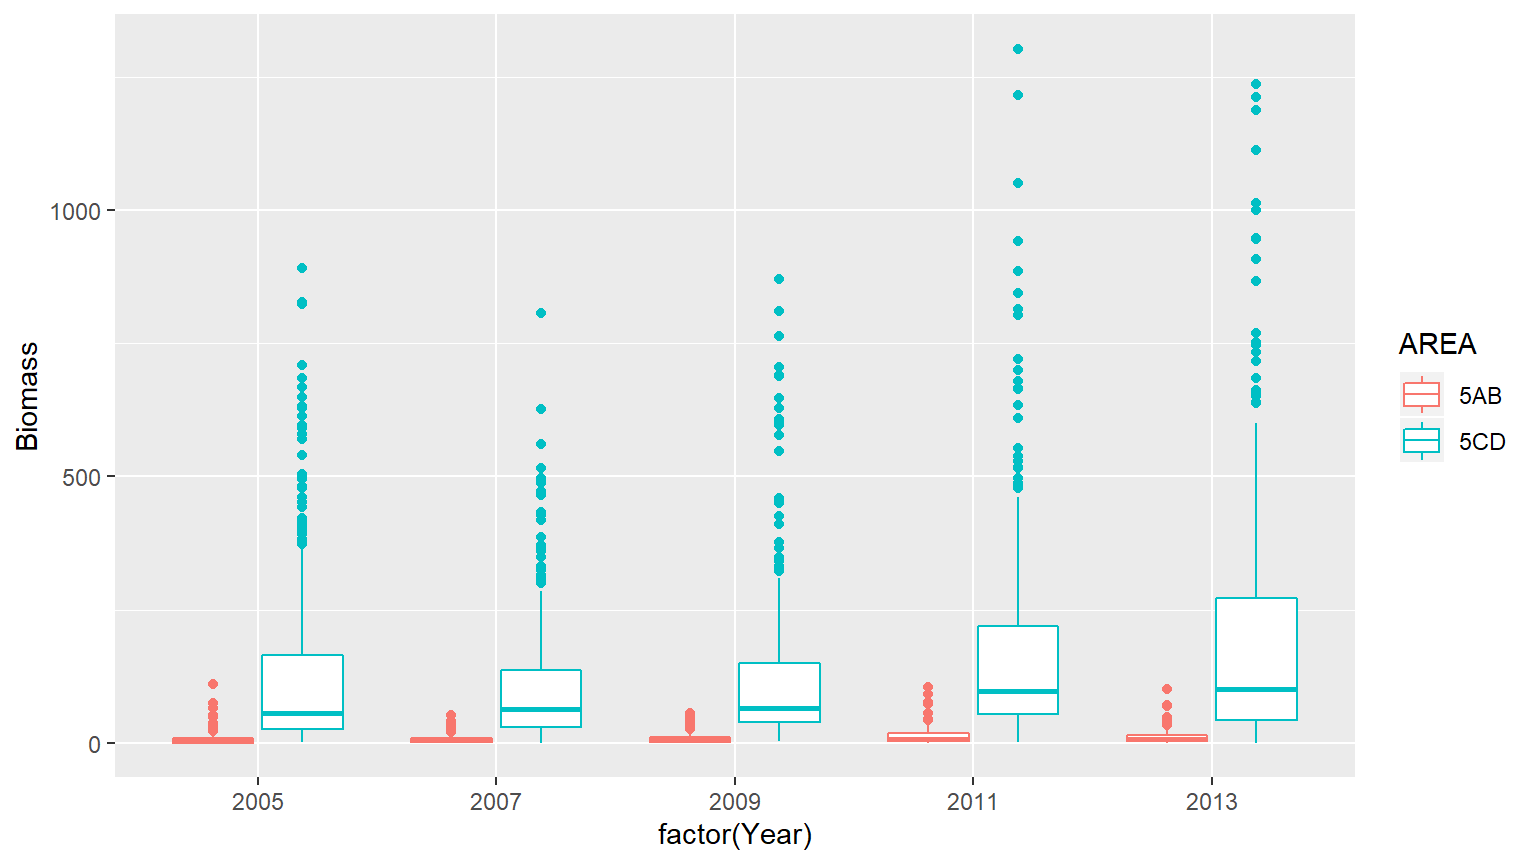
\includegraphics[width=.9\linewidth]{figure/boxplot_TSf_AREA-1} 

}



\end{knitrout}
\end{frame}


\begin{frame}[fragile]{Boxplot: x-axis changing label}
\begin{knitrout}\footnotesize
\definecolor{shadecolor}{rgb}{0.969, 0.969, 0.969}\color{fgcolor}\begin{kframe}
\begin{alltt}
\hlstd{boxplot_TS_AREA} \hlkwb{<-} \hlstd{boxplot_TS_AREA} \hlopt{+}
  \hlkwd{scale_x_discrete}\hlstd{(}\hlkwc{name}\hlstd{=}\hlkwa{NULL}\hlstd{,}
                   \hlkwc{breaks}\hlstd{=}\hlkwd{c}\hlstd{(}\hlstr{"2005"}\hlstd{,} \hlstr{"2009"}\hlstd{,} \hlstr{"2013"}\hlstd{),}
                   \hlkwc{labels}\hlstd{=}\hlkwd{c}\hlstd{(}\hlstr{"Year-2005"}\hlstd{,} \hlstr{"Year-2009"}\hlstd{,} \hlstr{"Year-2013"}\hlstd{))}
\hlkwd{print}\hlstd{(boxplot_TS_AREA)}
\end{alltt}
\end{kframe}

{\centering \includegraphics[width=.9\linewidth]{figure/boxplot_TSf_AREA_xaxis-1} 

}



\end{knitrout}
\end{frame}



\begin{frame}[fragile]{Boxplot (and all other plots): changing label in the legend}
The easiest way to change the label in the legend (i.e. 5AB and 5CD) rename the factor levels before the plot:

\begin{knitrout}\footnotesize
\definecolor{shadecolor}{rgb}{0.969, 0.969, 0.969}\color{fgcolor}\begin{kframe}
\begin{alltt}
\hlstd{df_data}\hlopt{$}\hlstd{AREA} \hlkwb{<-} \hlkwd{factor}\hlstd{(df_data}\hlopt{$}\hlstd{AREA,} \hlkwc{levels}\hlstd{=}\hlkwd{c}\hlstd{(}\hlstr{"5AB"}\hlstd{,} \hlstr{"5CD"}\hlstd{),}
                       \hlkwc{labels}\hlstd{=}\hlkwd{c}\hlstd{(}\hlstr{"Northern area"}\hlstd{,} \hlstr{"Southern area"}\hlstd{))}
\end{alltt}
\end{kframe}
\end{knitrout}

This code can also be useful for reordering the factor levels before the plot:
\begin{knitrout}\footnotesize
\definecolor{shadecolor}{rgb}{0.969, 0.969, 0.969}\color{fgcolor}\begin{kframe}
\begin{alltt}
\hlstd{df_data}\hlopt{$}\hlstd{AREA} \hlkwb{<-} \hlkwd{factor}\hlstd{(df_data}\hlopt{$}\hlstd{AREA,} \hlkwc{levels}\hlstd{=}\hlkwd{c}\hlstd{(}\hlstr{"5CD"}\hlstd{,} \hlstr{"5AB"}\hlstd{),}
                       \hlkwc{labels}\hlstd{=}\hlkwd{c}\hlstd{(}\hlstr{"Southern area"}\hlstd{,} \hlstr{"Northern area"}\hlstd{))}
\end{alltt}
\end{kframe}
\end{knitrout}
\end{frame}

\begin{frame}[fragile]{Boxplot with changed factor label}
\begin{knitrout}\footnotesize
\definecolor{shadecolor}{rgb}{0.969, 0.969, 0.969}\color{fgcolor}\begin{kframe}
\begin{alltt}
\hlstd{bplot_TS} \hlkwb{<-} \hlkwd{ggplot}\hlstd{(df_data,} \hlkwd{aes}\hlstd{(}\hlkwc{x}\hlstd{=}\hlkwd{factor}\hlstd{(Year),} \hlkwc{y}\hlstd{=Biomass,} \hlkwc{colour}\hlstd{=AREA))} \hlopt{+}
  \hlkwd{geom_boxplot}\hlstd{()} \hlopt{+}
  \hlkwd{scale_x_discrete}\hlstd{(}\hlkwc{name}\hlstd{=}\hlkwa{NULL}\hlstd{,}
                   \hlkwc{breaks}\hlstd{=}\hlkwd{c}\hlstd{(}\hlstr{"2005"}\hlstd{,} \hlstr{"2009"}\hlstd{,} \hlstr{"2013"}\hlstd{),}
                   \hlkwc{labels}\hlstd{=}\hlkwd{c}\hlstd{(}\hlstr{"Year-2005"}\hlstd{,} \hlstr{"Year-2009"}\hlstd{,} \hlstr{"Year-2013"}\hlstd{))} \hlopt{+}
  \hlkwd{scale_color_manual}\hlstd{(}\hlkwc{name}\hlstd{=}\hlstr{'Area'}\hlstd{,} \hlkwc{values} \hlstd{= cb_palette_black)} \hlopt{+}
  \hlkwd{theme}\hlstd{(}\hlkwc{legend.position}\hlstd{=}\hlkwd{c}\hlstd{(}\hlnum{0.2}\hlstd{,}\hlnum{0.9}\hlstd{))}
\hlkwd{print}\hlstd{(bplot_TS)}
\end{alltt}
\end{kframe}

{\centering \includegraphics[width=.9\linewidth]{figure/boxplot_TSf_AREA_final-1} 

}



\end{knitrout}

\end{frame}

%%%%%%%%%%%%%%%%%%%%%%%%%%%%%%%%%%%%%%%%%%%%%%%%%%%%%%%%%%%%%%%%%%%%%%%%%%%%%%%%
%% facet
%%%%%%%%%%%%%%%%%%%%%%%%%%%%%%%%%%%%%%%%%%%%%%%%%%%%%%%%%%%%%%%%%%%%%%%%%%%%%%%%
\section{Faceting}

%%%%%%%%%%%%%%%%%%%%%%%%%%%%%%%%%%%%%
\subsection{\lstinline{facet_wrap}}
\begin{frame}[fragile]{Faceting: \lstinline{facet_wrap}}
\begin{knitrout}\footnotesize
\definecolor{shadecolor}{rgb}{0.969, 0.969, 0.969}\color{fgcolor}\begin{kframe}
\begin{alltt}
\hlstd{hist} \hlkwb{<-} \hlkwd{ggplot}\hlstd{(}\hlkwc{data}\hlstd{=df_data,} \hlkwd{aes}\hlstd{(}\hlkwc{x}\hlstd{=DURATION_MINUTES,} \hlkwc{fill}\hlstd{=AREA))} \hlopt{+}
  \hlkwd{geom_histogram}\hlstd{()}
\hlkwd{print}\hlstd{(hist)}
\end{alltt}


{\ttfamily\noindent\itshape\color{messagecolor}{\#\# `stat\_bin()` using `bins = 30`. Pick better value with `binwidth`.}}\end{kframe}

{\centering \includegraphics[width=.9\linewidth]{figure/facet_wrap_0-1} 

}



\end{knitrout}
\end{frame}

\begin{frame}[fragile]{Faceting: \lstinline{facet_wrap}}
\begin{knitrout}\footnotesize
\definecolor{shadecolor}{rgb}{0.969, 0.969, 0.969}\color{fgcolor}\begin{kframe}
\begin{alltt}
\hlstd{fw1} \hlkwb{<-} \hlkwd{ggplot}\hlstd{(}\hlkwc{data}\hlstd{=df_data,} \hlkwd{aes}\hlstd{(}\hlkwc{x}\hlstd{=DURATION_MINUTES))} \hlopt{+}
  \hlkwd{geom_histogram}\hlstd{(}\hlkwc{binwidth}\hlstd{=}\hlnum{1}\hlstd{)} \hlopt{+} \hlkwd{facet_wrap}\hlstd{(}\hlopt{~} \hlstd{AREA)}
\hlkwd{print}\hlstd{(fw1)}
\end{alltt}
\end{kframe}

{\centering \includegraphics[width=.9\linewidth]{figure/facet_wrap_1-1} 

}



\end{knitrout}
\end{frame}

\begin{frame}[fragile]{\lstinline{facet_wrap}: free scales}
\begin{knitrout}\footnotesize
\definecolor{shadecolor}{rgb}{0.969, 0.969, 0.969}\color{fgcolor}\begin{kframe}
\begin{alltt}
\hlstd{fw1_free} \hlkwb{<-} \hlkwd{ggplot}\hlstd{(}\hlkwc{data}\hlstd{=df_data,} \hlkwd{aes}\hlstd{(}\hlkwc{x}\hlstd{=DURATION_MINUTES))} \hlopt{+}
  \hlkwd{geom_histogram}\hlstd{(}\hlkwc{binwidth}\hlstd{=}\hlnum{1}\hlstd{)} \hlopt{+} \hlkwd{facet_wrap}\hlstd{(}\hlopt{~} \hlstd{AREA ,} \hlkwc{scales} \hlstd{=} \hlstr{'free'}\hlstd{)}
\hlkwd{print}\hlstd{(fw1_free)}
\end{alltt}
\end{kframe}

{\centering \includegraphics[width=.9\linewidth]{figure/facet_wrap_2-1} 

}



\end{knitrout}
\end{frame}

\begin{frame}[fragile]{\lstinline{facet_wrap}: free y scale}
\begin{knitrout}\footnotesize
\definecolor{shadecolor}{rgb}{0.969, 0.969, 0.969}\color{fgcolor}\begin{kframe}
\begin{alltt}
\hlstd{fw1_free_y} \hlkwb{<-} \hlkwd{ggplot}\hlstd{(}\hlkwc{data}\hlstd{=df_data,} \hlkwd{aes}\hlstd{(}\hlkwc{x}\hlstd{=DURATION_MINUTES))} \hlopt{+}
  \hlkwd{geom_histogram}\hlstd{(}\hlkwc{binwidth}\hlstd{=}\hlnum{1}\hlstd{)} \hlopt{+} \hlkwd{facet_wrap}\hlstd{(}\hlopt{~} \hlstd{AREA ,} \hlkwc{scales} \hlstd{=} \hlstr{'free_y'}\hlstd{)}
\hlkwd{print}\hlstd{(fw1_free_y)}
\end{alltt}
\end{kframe}

{\centering \includegraphics[width=.9\linewidth]{figure/facet_wrap_3-1} 

}



\end{knitrout}
\end{frame}

\begin{frame}[fragile]{\lstinline{facet_wrap}: free y scale}
\begin{knitrout}\footnotesize
\definecolor{shadecolor}{rgb}{0.969, 0.969, 0.969}\color{fgcolor}\begin{kframe}
\begin{alltt}
\hlstd{fw1_col} \hlkwb{<-} \hlkwd{ggplot}\hlstd{(}\hlkwc{data}\hlstd{=df_data,} \hlkwd{aes}\hlstd{(}\hlkwc{x}\hlstd{=DURATION_MINUTES))} \hlopt{+}
  \hlkwd{geom_histogram}\hlstd{(}\hlkwc{binwidth}\hlstd{=}\hlnum{1}\hlstd{)} \hlopt{+}
  \hlkwd{facet_wrap}\hlstd{(}\hlopt{~} \hlstd{AREA,} \hlkwc{ncol} \hlstd{=} \hlnum{1}\hlstd{,} \hlkwc{nrow} \hlstd{=} \hlnum{2}\hlstd{,} \hlkwc{scales} \hlstd{=} \hlstr{'fixed'}\hlstd{)}
\hlkwd{print}\hlstd{(fw1_col)}
\end{alltt}
\end{kframe}

{\centering \includegraphics[width=.9\linewidth]{figure/facet_wrap_4-1} 

}



\end{knitrout}
\end{frame}

\begin{frame}[fragile]{\lstinline{facet_wrap}: free y scale}
\begin{knitrout}\footnotesize
\definecolor{shadecolor}{rgb}{0.969, 0.969, 0.969}\color{fgcolor}\begin{kframe}
\begin{alltt}
\hlstd{fw2} \hlkwb{<-} \hlkwd{ggplot}\hlstd{(}\hlkwc{data}\hlstd{=df_data,} \hlkwd{aes}\hlstd{(}\hlkwc{x}\hlstd{=DURATION_MINUTES))} \hlopt{+}
  \hlkwd{geom_histogram}\hlstd{(}\hlkwc{binwidth}\hlstd{=}\hlnum{1}\hlstd{)} \hlopt{+} \hlkwd{facet_wrap}\hlstd{(}\hlopt{~} \hlstd{AREA} \hlopt{+} \hlstd{Year_fac)}
\hlkwd{print}\hlstd{(fw2)}
\end{alltt}
\end{kframe}

{\centering \includegraphics[width=.9\linewidth]{figure/facet_wrap_5-1} 

}



\end{knitrout}
\end{frame}

\begin{frame}[fragile]{\lstinline{facet_wrap}: free y scale}
\begin{knitrout}\footnotesize
\definecolor{shadecolor}{rgb}{0.969, 0.969, 0.969}\color{fgcolor}\begin{kframe}
\begin{alltt}
\hlstd{fw2_2} \hlkwb{<-} \hlkwd{ggplot}\hlstd{(}\hlkwc{data}\hlstd{=df_data,} \hlkwd{aes}\hlstd{(}\hlkwc{x}\hlstd{=DURATION_MINUTES))} \hlopt{+}
  \hlkwd{geom_histogram}\hlstd{(}\hlkwc{binwidth}\hlstd{=}\hlnum{1}\hlstd{)} \hlopt{+} \hlkwd{facet_wrap}\hlstd{(} \hlopt{~} \hlstd{Year_fac} \hlopt{+} \hlstd{AREA)}
\hlkwd{print}\hlstd{(fw2_2)}
\end{alltt}
\end{kframe}

{\centering \includegraphics[width=.9\linewidth]{figure/facet_wrap_6-1} 

}



\end{knitrout}
\end{frame}

%%%%%%%%%%%%%%%%%%%%%%%%%%%%%%%%%%%%%
\subsection{\lstinline{facet_grid}}

\begin{frame}[fragile]{\lstinline{facet_grid}: more flexible}
\begin{knitrout}\footnotesize
\definecolor{shadecolor}{rgb}{0.969, 0.969, 0.969}\color{fgcolor}\begin{kframe}
\begin{alltt}
\hlstd{fg1_1} \hlkwb{<-} \hlkwd{ggplot}\hlstd{(df_data,} \hlkwd{aes}\hlstd{(}\hlkwc{x}\hlstd{=Avg_net_depth,} \hlkwc{y}\hlstd{=nFish,} \hlkwc{color}\hlstd{=AREA))} \hlopt{+}
  \hlkwd{geom_point}\hlstd{(}\hlkwc{shape}\hlstd{=}\hlnum{20}\hlstd{)} \hlopt{+} \hlkwd{facet_grid}\hlstd{(.} \hlopt{~} \hlstd{Year)}
\hlkwd{print}\hlstd{(fg1_1)}
\end{alltt}
\end{kframe}

{\centering \includegraphics[width=.9\linewidth]{figure/facet_grid_1-1} 

}



\end{knitrout}
\end{frame}

\begin{frame}[fragile]{\lstinline{facet_grid}: change faceting display}
\begin{knitrout}\footnotesize
\definecolor{shadecolor}{rgb}{0.969, 0.969, 0.969}\color{fgcolor}\begin{kframe}
\begin{alltt}
\hlstd{fg1_2} \hlkwb{<-} \hlkwd{ggplot}\hlstd{(df_data,} \hlkwd{aes}\hlstd{(}\hlkwc{x}\hlstd{=Avg_net_depth,} \hlkwc{y}\hlstd{=nFish,} \hlkwc{color}\hlstd{=AREA))} \hlopt{+}
  \hlkwd{geom_point}\hlstd{(}\hlkwc{shape}\hlstd{=}\hlnum{20}\hlstd{)} \hlopt{+} \hlkwd{facet_grid}\hlstd{(Year} \hlopt{~} \hlstd{.)}
\hlkwd{print}\hlstd{(fg1_2)}
\end{alltt}
\end{kframe}

{\centering \includegraphics[width=.9\linewidth]{figure/facet_grid_2-1} 

}



\end{knitrout}
\end{frame}


\begin{frame}[fragile]{\lstinline{facet_grid}: facet with all the data}
\begin{knitrout}\footnotesize
\definecolor{shadecolor}{rgb}{0.969, 0.969, 0.969}\color{fgcolor}\begin{kframe}
\begin{alltt}
\hlstd{fg1_3} \hlkwb{<-} \hlkwd{ggplot}\hlstd{(df_data,} \hlkwd{aes}\hlstd{(}\hlkwc{x}\hlstd{=Avg_net_depth,} \hlkwc{y}\hlstd{=nFish,} \hlkwc{color}\hlstd{=AREA))} \hlopt{+}
  \hlkwd{geom_point}\hlstd{(}\hlkwc{shape}\hlstd{=}\hlnum{20}\hlstd{)} \hlopt{+} \hlkwd{facet_grid}\hlstd{(Year} \hlopt{~} \hlstd{.,} \hlkwc{margins} \hlstd{=} \hlnum{TRUE}\hlstd{)}
\hlkwd{print}\hlstd{(fg1_3)}
\end{alltt}
\end{kframe}

{\centering \includegraphics[width=.9\linewidth]{figure/facet_grid_3-1} 

}



\end{knitrout}
\end{frame}

\begin{frame}[fragile]{\lstinline{facet_grid}: two faceting factors}
\begin{knitrout}\footnotesize
\definecolor{shadecolor}{rgb}{0.969, 0.969, 0.969}\color{fgcolor}\begin{kframe}
\begin{alltt}
\hlstd{fg2_1} \hlkwb{<-} \hlkwd{ggplot}\hlstd{(df_data,} \hlkwd{aes}\hlstd{(}\hlkwc{x}\hlstd{=Avg_net_depth,} \hlkwc{y}\hlstd{=nFish))} \hlopt{+}
  \hlkwd{geom_point}\hlstd{(}\hlkwc{shape}\hlstd{=}\hlnum{20}\hlstd{)} \hlopt{+} \hlkwd{facet_grid}\hlstd{(}\hlopt{~} \hlstd{Year} \hlopt{+} \hlstd{AREA)}
\hlkwd{print}\hlstd{(fg2_1)}
\end{alltt}
\end{kframe}

{\centering \includegraphics[width=.9\linewidth]{figure/facet_grid_4-1} 

}



\end{knitrout}
\end{frame}

\begin{frame}[fragile]{\lstinline{facet_grid}: two faceting factors}
\begin{knitrout}\footnotesize
\definecolor{shadecolor}{rgb}{0.969, 0.969, 0.969}\color{fgcolor}\begin{kframe}
\begin{alltt}
\hlstd{fg2_2} \hlkwb{<-} \hlkwd{ggplot}\hlstd{(df_data,} \hlkwd{aes}\hlstd{(}\hlkwc{x}\hlstd{=Avg_net_depth,} \hlkwc{y}\hlstd{=nFish))} \hlopt{+}
  \hlkwd{geom_point}\hlstd{(}\hlkwc{shape}\hlstd{=}\hlnum{20}\hlstd{)} \hlopt{+} \hlkwd{facet_grid}\hlstd{(AREA} \hlopt{~} \hlstd{Year)}
\hlkwd{print}\hlstd{(fg2_2)}
\end{alltt}
\end{kframe}

{\centering \includegraphics[width=.9\linewidth]{figure/facet_grid_5-1} 

}



\end{knitrout}
\end{frame}



\begin{frame}[fragile]{\lstinline{facet_grid}: scales and space free}
\begin{knitrout}\footnotesize
\definecolor{shadecolor}{rgb}{0.969, 0.969, 0.969}\color{fgcolor}\begin{kframe}
\begin{alltt}
\hlstd{fg2_3} \hlkwb{<-} \hlkwd{ggplot}\hlstd{(df_data,} \hlkwd{aes}\hlstd{(}\hlkwc{x}\hlstd{=Avg_net_depth,} \hlkwc{y}\hlstd{=nFish))} \hlopt{+}
  \hlkwd{geom_point}\hlstd{(}\hlkwc{shape}\hlstd{=}\hlnum{20}\hlstd{,} \hlkwc{size}\hlstd{=}\hlnum{1}\hlstd{)} \hlopt{+}
  \hlkwd{facet_grid}\hlstd{(AREA} \hlopt{~} \hlstd{Year,} \hlkwc{scales}\hlstd{=}\hlstr{'free'}\hlstd{,} \hlkwc{space} \hlstd{=} \hlstr{'free'}\hlstd{)}
\hlkwd{print}\hlstd{(fg2_3)}
\end{alltt}
\end{kframe}

{\centering \includegraphics[width=.9\linewidth]{figure/facet_grid_6-1} 

}



\end{knitrout}
\end{frame}

\begin{frame}[fragile]{\lstinline{facet_grid}: renaming labels}
Replace manually names factor:
\begin{knitrout}\footnotesize
\definecolor{shadecolor}{rgb}{0.969, 0.969, 0.969}\color{fgcolor}\begin{kframe}
\begin{alltt}
\hlkwd{levels}\hlstd{(df_data}\hlopt{$}\hlstd{AREA)} \hlkwb{<-} \hlkwd{c}\hlstd{(}\hlstr{'Northern area'}\hlstd{,} \hlstr{'Southern area'}\hlstd{)}
\end{alltt}
\end{kframe}
\end{knitrout}
Or write a function:
\begin{knitrout}\footnotesize
\definecolor{shadecolor}{rgb}{0.969, 0.969, 0.969}\color{fgcolor}\begin{kframe}
\begin{alltt}
\hlcom{## string is the levels of a factor}
\hlstd{fn_alphabetic_label} \hlkwb{<-} \hlkwa{function}\hlstd{(}\hlkwc{string}\hlstd{)\{}
  \hlkwa{for} \hlstd{( i} \hlkwa{in} \hlnum{1}\hlopt{:}\hlkwd{length}\hlstd{(string))\{}
    \hlstd{string[i]} \hlkwb{<-} \hlstd{letters[i]}
  \hlstd{\}}
  \hlkwd{return}\hlstd{(string)}
\hlstd{\}}
\end{alltt}
\end{kframe}
\end{knitrout}
\end{frame}


\begin{frame}[fragile]{\lstinline{facet_grid}: renaming labels}
\begin{knitrout}\footnotesize
\definecolor{shadecolor}{rgb}{0.969, 0.969, 0.969}\color{fgcolor}\begin{kframe}
\begin{alltt}
\hlstd{fg1_3a} \hlkwb{<-} \hlkwd{ggplot}\hlstd{(df_data,} \hlkwd{aes}\hlstd{(}\hlkwc{x}\hlstd{=Avg_net_depth,} \hlkwc{y}\hlstd{=nFish,} \hlkwc{color}\hlstd{=AREA))} \hlopt{+}
  \hlkwd{geom_point}\hlstd{(}\hlkwc{shape}\hlstd{=}\hlnum{20}\hlstd{,} \hlkwc{size}\hlstd{=}\hlnum{1}\hlstd{)} \hlopt{+}
  \hlkwd{facet_grid}\hlstd{(Year} \hlopt{~} \hlstd{.,} \hlkwc{labeller} \hlstd{=} \hlkwd{labeller}\hlstd{(}\hlkwc{Year} \hlstd{= fn_alphabetic_label))}
\hlkwd{print}\hlstd{(fg1_3a)}
\end{alltt}
\end{kframe}

{\centering \includegraphics[width=.9\linewidth]{figure/facet_grid_9-1} 

}



\end{knitrout}
\end{frame}



\begin{frame}[fragile]{\lstinline{facet_grid}: changing facets}
\begin{knitrout}\footnotesize
\definecolor{shadecolor}{rgb}{0.969, 0.969, 0.969}\color{fgcolor}\begin{kframe}
\begin{alltt}
\hlstd{fg2_3b} \hlkwb{<-} \hlstd{fg2_2} \hlopt{+}
  \hlkwd{theme}\hlstd{(}\hlkwc{strip.text.x} \hlstd{=} \hlkwd{element_text}\hlstd{(}\hlkwc{size}\hlstd{=}\hlnum{8}\hlstd{,} \hlkwc{angle}\hlstd{=}\hlnum{45}\hlstd{),}
        \hlkwc{strip.text.y} \hlstd{=} \hlkwd{element_text}\hlstd{(}\hlkwc{size}\hlstd{=}\hlnum{12}\hlstd{,} \hlkwc{face}\hlstd{=}\hlstr{"bold"}\hlstd{),}
        \hlkwc{strip.background} \hlstd{=} \hlkwd{element_rect}\hlstd{(}\hlkwc{colour}\hlstd{=}\hlstr{"red"}\hlstd{,} \hlkwc{fill}\hlstd{=}\hlnum{NA}\hlstd{))}
\hlkwd{print}\hlstd{(fg2_3b)}
\end{alltt}
\end{kframe}

{\centering \includegraphics[width=.9\linewidth]{figure/facet_grid_10-1} 

}



\end{knitrout}
\end{frame}

%%%%%%%%%%%%%%%%%%%%%%%%%%%%%%%%%%%%%%%%%%%%%%%%%%%%%%%%%%%%%%%%%%%%%%%%%%%%%%%%
%% Multiple-plots
%%%%%%%%%%%%%%%%%%%%%%%%%%%%%%%%%%%%%%%%%%%%%%%%%%%%%%%%%%%%%%%%%%%%%%%%%%%%%%%%
\section{Multiple-plots}
\begin{frame}[fragile]{Multiple (different) plots}
It can be hard to plot on the same page different plots.

For example, it is not possible to plot on the same page a boxplot, a scatter plot, and a bar plot.

\begin{knitrout}\footnotesize
\definecolor{shadecolor}{rgb}{0.969, 0.969, 0.969}\color{fgcolor}\begin{kframe}
\begin{alltt}
\hlkwd{source}\hlstd{(}\hlstr{'R/Fun/gg_multiplot.R'}\hlstd{)}
\hlkwd{gg_multiplot}\hlstd{(}\hlkwc{plotlist} \hlstd{=} \hlkwd{list}\hlstd{(sp_c_wanderson, boxplot_TS_AREA,}
                             \hlstd{TSplot_i95))}
\end{alltt}
\end{kframe}
\end{knitrout}
\end{frame}

\begin{frame}[fragile]{Multiple (different) plots}
\begin{knitrout}\footnotesize
\definecolor{shadecolor}{rgb}{0.969, 0.969, 0.969}\color{fgcolor}

{\centering \includegraphics[width=.9\linewidth]{figure/multi_plot2-1} 

}



\end{knitrout}
\end{frame}

\begin{frame}[fragile]{Multiple (different) plots}
%Choose the layout to 
\begin{knitrout}\footnotesize
\definecolor{shadecolor}{rgb}{0.969, 0.969, 0.969}\color{fgcolor}\begin{kframe}
\begin{alltt}
\hlkwd{gg_multiplot}\hlstd{(}\hlkwc{plotlist} \hlstd{=} \hlkwd{list}\hlstd{(sp_c_wanderson} \hlopt{+} \hlkwd{ggtitle}\hlstd{(}\hlstr{'(a)'}\hlstd{),}
                             \hlstd{boxplot_TS_AREA} \hlopt{+} \hlkwd{ggtitle}\hlstd{(}\hlstr{'(b)'}\hlstd{),}
                             \hlstd{TSplot_i95} \hlopt{+} \hlkwd{ggtitle}\hlstd{(}\hlstr{'(c)'}\hlstd{)),}
             \hlkwc{layout} \hlstd{=} \hlkwd{matrix}\hlstd{(}\hlkwd{c}\hlstd{(}\hlnum{1}\hlstd{,}\hlnum{2}\hlstd{,}\hlnum{3}\hlstd{,}\hlnum{3}\hlstd{),} \hlkwc{nrow}\hlstd{=}\hlnum{2}\hlstd{,} \hlkwc{byrow}\hlstd{=}\hlnum{TRUE}\hlstd{))}
\end{alltt}
\end{kframe}
\end{knitrout}
\end{frame}

\begin{frame}[fragile]{Multiple (different) plots}
\begin{knitrout}\footnotesize
\definecolor{shadecolor}{rgb}{0.969, 0.969, 0.969}\color{fgcolor}

{\centering \includegraphics[width=.9\linewidth]{figure/multi_plot4-1} 

}



\end{knitrout}
\end{frame}



%%%%%%%%%%%%%%%%%%%%%%%%%%%%%%%%%%%%%%%%%%%%%%%%%%%%%%%%%%%%%%%%%%%%%%%%%%%%%%%%
%% Theme
%%%%%%%%%%%%%%%%%%%%%%%%%%%%%%%%%%%%%%%%%%%%%%%%%%%%%%%%%%%%%%%%%%%%%%%%%%%%%%%%
\section{Theme}
\begin{frame}{Theme}
\begin{itemize}
\item ggplot2 uses a theme which controls the background, fonts, text size, ...
\item change the theme for the current R session: \lstinline{theme_set(theme_gray())}
\item create or update your own theme : \newline
\lstinline{p + theme(plot.background = element_rect(fill = "darkblue"))}
\end{itemize}
\end{frame}

\begin{frame}[fragile]{Theme: background change}
\begin{knitrout}\footnotesize
\definecolor{shadecolor}{rgb}{0.969, 0.969, 0.969}\color{fgcolor}\begin{kframe}
\begin{alltt}
\hlkwd{print}\hlstd{(fg2_2} \hlopt{+}
        \hlkwd{theme}\hlstd{(}\hlkwc{plot.background} \hlstd{=} \hlkwd{element_rect}\hlstd{(}\hlkwc{fill} \hlstd{=} \hlstr{"darkblue"}\hlstd{)))}
\end{alltt}
\end{kframe}

{\centering \includegraphics[width=.9\linewidth]{figure/theme_1-1} 

}



\end{knitrout}
\end{frame}

\begin{frame}[fragile]{Theme: black and white}
\begin{knitrout}\footnotesize
\definecolor{shadecolor}{rgb}{0.969, 0.969, 0.969}\color{fgcolor}\begin{kframe}
\begin{alltt}
\hlkwd{print}\hlstd{(fg2_2} \hlopt{+} \hlkwd{theme_bw}\hlstd{())}
\end{alltt}
\end{kframe}

{\centering \includegraphics[width=.9\linewidth]{figure/theme_2-1} 

}



\end{knitrout}
\end{frame}

\begin{frame}[fragile]{Theme: classic}
\begin{knitrout}\footnotesize
\definecolor{shadecolor}{rgb}{0.969, 0.969, 0.969}\color{fgcolor}\begin{kframe}
\begin{alltt}
\hlkwd{print}\hlstd{(fg2_2} \hlopt{+} \hlkwd{theme_classic}\hlstd{())}
\end{alltt}
\end{kframe}

{\centering \includegraphics[width=.9\linewidth]{figure/theme_3-1} 

}



\end{knitrout}
\end{frame}

\begin{frame}[fragile]{Theme: minimalist}
\begin{knitrout}\footnotesize
\definecolor{shadecolor}{rgb}{0.969, 0.969, 0.969}\color{fgcolor}\begin{kframe}
\begin{alltt}
\hlkwd{print}\hlstd{(fg2_2} \hlopt{+}  \hlkwd{theme_minimal}\hlstd{())}
\end{alltt}
\end{kframe}

{\centering \includegraphics[width=.9\linewidth]{figure/theme_4-1} 

}



\end{knitrout}
\end{frame}


\begin{frame}[fragile]{Theme: minimalist tufte}
\begin{knitrout}\footnotesize
\definecolor{shadecolor}{rgb}{0.969, 0.969, 0.969}\color{fgcolor}\begin{kframe}
\begin{alltt}
\hlkwd{library}\hlstd{(ggthemes)}
\hlkwd{print}\hlstd{(fg2_2} \hlopt{+}  \hlkwd{theme_tufte}\hlstd{())}
\end{alltt}
\end{kframe}

{\centering \includegraphics[width=.9\linewidth]{figure/theme_5-1} 

}



\end{knitrout}
\end{frame}


\begin{frame}[fragile]{Theme: the economist}
\begin{knitrout}\footnotesize
\definecolor{shadecolor}{rgb}{0.969, 0.969, 0.969}\color{fgcolor}\begin{kframe}
\begin{alltt}
\hlkwd{library}\hlstd{(ggthemes)}
\hlkwd{print}\hlstd{(fg2_2} \hlopt{+} \hlkwd{theme_economist}\hlstd{())}
\end{alltt}
\end{kframe}

{\centering \includegraphics[width=.9\linewidth]{figure/theme_6-1} 

}



\end{knitrout}
\end{frame}

\begin{frame}[fragile]{Theme: make your own}
\begin{knitrout}\footnotesize
\definecolor{shadecolor}{rgb}{0.969, 0.969, 0.969}\color{fgcolor}\begin{kframe}
\begin{alltt}
\hlkwd{theme_update}\hlstd{(}\hlkwc{axis.text} \hlstd{=} \hlkwd{element_text}\hlstd{(}\hlkwc{size} \hlstd{=} \hlkwd{rel}\hlstd{(}\hlnum{0.8}\hlstd{)),}
             \hlkwc{axis.ticks} \hlstd{=} \hlkwd{element_line}\hlstd{(}\hlkwc{colour} \hlstd{=} \hlstr{"black"}\hlstd{,} \hlkwc{size}\hlstd{=}\hlnum{1}\hlstd{),}
             \hlkwc{axis.line} \hlstd{=} \hlkwd{element_line}\hlstd{(),}
             \hlkwc{panel.background} \hlstd{=} \hlkwd{element_rect}\hlstd{(}\hlkwc{fill} \hlstd{=} \hlnum{NA}\hlstd{,} \hlkwc{colour} \hlstd{=} \hlnum{NA}\hlstd{),}
             \hlkwc{panel.border} \hlstd{=} \hlkwd{element_rect}\hlstd{(}\hlkwc{fill} \hlstd{=} \hlnum{NA}\hlstd{,} \hlkwc{colour} \hlstd{=} \hlnum{NA}\hlstd{),}
             \hlkwc{panel.grid.major} \hlstd{=} \hlkwd{element_line}\hlstd{(}\hlkwc{colour} \hlstd{=} \hlstr{"grey90"}\hlstd{,} \hlkwc{size} \hlstd{=} \hlnum{0.2}\hlstd{),}
             \hlkwc{panel.grid.minor} \hlstd{=} \hlkwd{element_line}\hlstd{(}\hlkwc{colour} \hlstd{=} \hlnum{NA}\hlstd{,} \hlkwc{size} \hlstd{=} \hlnum{0.5}\hlstd{),}
             \hlkwc{strip.background} \hlstd{=} \hlkwd{element_rect}\hlstd{(}\hlkwc{fill} \hlstd{=} \hlstr{"grey80"}\hlstd{,}\hlkwc{colour} \hlstd{=} \hlstr{"grey50"}\hlstd{),}
             \hlkwc{strip.background} \hlstd{=} \hlkwd{element_rect}\hlstd{(}\hlkwc{fill} \hlstd{=} \hlstr{"grey80"}\hlstd{,}\hlkwc{colour} \hlstd{=} \hlstr{"grey50"}\hlstd{),}
             \hlkwc{panel.background} \hlstd{=} \hlkwd{element_rect}\hlstd{(}\hlkwc{fill} \hlstd{=} \hlstr{"transparent"}\hlstd{,} \hlkwc{colour} \hlstd{=} \hlnum{NA}\hlstd{),}
             \hlkwc{panel.grid.minor} \hlstd{=} \hlkwd{element_blank}\hlstd{(),}
             \hlkwc{plot.background} \hlstd{=} \hlkwd{element_rect}\hlstd{(}\hlkwc{fill} \hlstd{=} \hlstr{"transparent"}\hlstd{,} \hlkwc{colour} \hlstd{=} \hlnum{NA}\hlstd{),}
             \hlkwc{legend.key} \hlstd{=} \hlkwd{element_rect}\hlstd{(}\hlkwc{colour} \hlstd{=} \hlstr{"grey80"}\hlstd{,} \hlkwc{fill}\hlstd{=} \hlstr{"grey80"}\hlstd{),}
             \hlkwc{legend.background} \hlstd{=} \hlkwd{element_rect}\hlstd{(}\hlkwc{colour} \hlstd{=} \hlstr{'black'}\hlstd{,} \hlkwc{fill} \hlstd{=} \hlnum{NA}\hlstd{),}
             \hlkwc{legend.key} \hlstd{=} \hlkwd{element_rect}\hlstd{(}\hlkwc{colour} \hlstd{=} \hlnum{NA}\hlstd{,}\hlkwc{fill}\hlstd{=}\hlnum{NA}\hlstd{),}
             \hlkwc{legend.key.size} \hlstd{=} \hlkwd{unit}\hlstd{(}\hlnum{1.1}\hlstd{,}\hlstr{'line'}\hlstd{),}
             \hlkwc{legend.title} \hlstd{=} \hlkwd{element_text}\hlstd{(}\hlkwc{size} \hlstd{=} \hlkwd{rel}\hlstd{(}\hlnum{1}\hlstd{),} \hlkwc{face} \hlstd{=} \hlstr{'bold'}\hlstd{),}
             \hlkwc{legend.text} \hlstd{=} \hlkwd{element_text}\hlstd{(}\hlkwc{size} \hlstd{=} \hlkwd{rel}\hlstd{(}\hlnum{1}\hlstd{)))}
\end{alltt}
\end{kframe}
\end{knitrout}
\end{frame}

%%%%%%%%%%%%%%%%%%%%%%%%%%%%%%%%%%%%%%%%%%%%%%%%%%%%%%%%%%%%%%%%%%%%%%%%%%%%%%%%
%%% Legend 
%%%%%%%%%%%%%%%%%%%%%%%%%%%%%%%%%%%%%%%%%%%%%%%%%%%%%%%%%%%%%%%%%%%%%%%%%%%%%%%%

\begin{frame}[fragile]{Legend position: top, bottom, left, right}
\begin{knitrout}\footnotesize
\definecolor{shadecolor}{rgb}{0.969, 0.969, 0.969}\color{fgcolor}\begin{kframe}
\begin{alltt}
\hlstd{sp_legend} \hlkwb{<-} \hlstd{sp_shape_imp2} \hlopt{+} \hlkwd{theme}\hlstd{(}\hlkwc{legend.position}\hlstd{=}\hlstr{"bottom"}\hlstd{,}
                                   \hlkwc{legend.box} \hlstd{=} \hlstr{"horizontal"}\hlstd{)}
\hlkwd{print}\hlstd{(sp_legend)}
\end{alltt}
\end{kframe}

{\centering \includegraphics[width=.9\linewidth]{figure/legend_p1-1} 

}



\end{knitrout}
\end{frame}

\begin{frame}[fragile]{Legend position: bottom left c(0,0), top right c(1,1)}
\begin{knitrout}\footnotesize
\definecolor{shadecolor}{rgb}{0.969, 0.969, 0.969}\color{fgcolor}\begin{kframe}
\begin{alltt}
\hlstd{sp_legend} \hlkwb{<-} \hlstd{sp_shape_imp2} \hlopt{+} \hlkwd{theme}\hlstd{(}\hlkwc{legend.position}\hlstd{=}\hlkwd{c}\hlstd{(}\hlnum{0.9}\hlstd{,}\hlnum{0.6}\hlstd{))}
\hlkwd{print}\hlstd{(sp_legend)}
\end{alltt}
\end{kframe}

{\centering \includegraphics[width=.9\linewidth]{figure/legend_p2-1} 

}



\end{knitrout}
\end{frame}

\begin{frame}[fragile]{Legend background}
\begin{knitrout}\footnotesize
\definecolor{shadecolor}{rgb}{0.969, 0.969, 0.969}\color{fgcolor}\begin{kframe}
\begin{alltt}
\hlstd{sp_legend2} \hlkwb{<-} \hlstd{sp_legend}  \hlopt{+}
  \hlkwd{theme}\hlstd{(}\hlkwc{legend.background} \hlstd{=} \hlkwd{element_rect}\hlstd{(}\hlkwc{fill}\hlstd{=}\hlstr{"lightblue"}\hlstd{,}
                                         \hlkwc{size}\hlstd{=}\hlnum{0.5}\hlstd{,} \hlkwc{linetype}\hlstd{=}\hlstr{"solid"}\hlstd{,}
                                         \hlkwc{colour} \hlstd{=}\hlstr{"darkblue"}\hlstd{))}
\hlkwd{print}\hlstd{(sp_legend2)}
\end{alltt}
\end{kframe}

{\centering \includegraphics[width=.9\linewidth]{figure/legend_b-1} 

}



\end{knitrout}
\end{frame}


\begin{frame}[fragile]{Legend order}
\begin{knitrout}\footnotesize
\definecolor{shadecolor}{rgb}{0.969, 0.969, 0.969}\color{fgcolor}\begin{kframe}
\begin{alltt}
\hlstd{sp_legend2} \hlkwb{<-} \hlstd{sp_legend2}  \hlopt{+}
  \hlkwd{guides}\hlstd{(}\hlkwc{shape} \hlstd{=} \hlkwd{guide_legend}\hlstd{(}\hlkwc{order}\hlstd{=}\hlnum{1}\hlstd{),}
         \hlkwc{color} \hlstd{=} \hlkwd{guide_legend}\hlstd{(}\hlkwc{order}\hlstd{=}\hlnum{2}\hlstd{))}
\hlkwd{print}\hlstd{(sp_legend2)}
\end{alltt}
\end{kframe}

{\centering \includegraphics[width=.9\linewidth]{figure/legend_order-1} 

}



\end{knitrout}
\end{frame}

\begin{frame}[fragile]{Remove legends}
\begin{knitrout}\footnotesize
\definecolor{shadecolor}{rgb}{0.969, 0.969, 0.969}\color{fgcolor}\begin{kframe}
\begin{alltt}
\hlstd{sp_legend2} \hlkwb{<-} \hlstd{sp_legend2}  \hlopt{+}
  \hlkwd{theme}\hlstd{(}\hlkwc{legend.position}\hlstd{=}\hlstr{'none'}\hlstd{)}
\hlkwd{print}\hlstd{(sp_legend2)}
\end{alltt}
\end{kframe}

{\centering \includegraphics[width=.9\linewidth]{figure/legend_rm-1} 

}



\end{knitrout}
\end{frame}

\begin{frame}[fragile]{Remove a specific legend}
\begin{knitrout}\footnotesize
\definecolor{shadecolor}{rgb}{0.969, 0.969, 0.969}\color{fgcolor}\begin{kframe}
\begin{alltt}
\hlstd{sp_legend_c} \hlkwb{<-} \hlstd{sp_legend} \hlopt{+}
  \hlkwd{guides}\hlstd{(}\hlkwc{color} \hlstd{=} \hlnum{FALSE}\hlstd{)}
\hlkwd{print}\hlstd{(sp_legend_c)}
\end{alltt}
\end{kframe}

{\centering \includegraphics[width=.9\linewidth]{figure/legend_rm2-1} 

}



\end{knitrout}
\end{frame}

%%%%%%%%%%%%%%%%%%%%%%%%%%%%%%%%%%%%%%%%%%%%%%%%%%%%%%%%%%%%%%%%%%%%%%%%%%%%%%%%
%% Saving
%%%%%%%%%%%%%%%%%%%%%%%%%%%%%%%%%%%%%%%%%%%%%%%%%%%%%%%%%%%%%%%%%%%%%%%%%%%%%%%%
\begin{frame}[fragile]{Saving a plot}
The ggsave function from ggplot2 package allows to automatically save a plot.
\begin{knitrout}\footnotesize
\definecolor{shadecolor}{rgb}{0.969, 0.969, 0.969}\color{fgcolor}\begin{kframe}
\begin{alltt}
\hlstd{sp_legend_c} \hlkwb{<-} \hlstd{sp_legend} \hlopt{+}
  \hlkwd{guides}\hlstd{(}\hlkwc{color} \hlstd{=} \hlnum{FALSE}\hlstd{)}
\hlkwd{print}\hlstd{(sp_legend_c)}

\hlkwd{ggsave}\hlstd{(}\hlkwc{plot}\hlstd{=sp_legend_c,} \hlkwc{filename} \hlstd{=} \hlstr{'sp_legend_c.pdf'}\hlstd{,} \hlkwc{path} \hlstd{=} \hlstr{'~/figure'}\hlstd{,}
       \hlkwc{width} \hlstd{=} \hlnum{8}\hlstd{,} \hlkwc{height} \hlstd{=} \hlnum{5}\hlstd{,} \hlkwc{units} \hlstd{=} \hlstr{'cm'}\hlstd{)}
\end{alltt}
\end{kframe}
\end{knitrout}
\end{frame}

%%%%%%%%%%%%%%%%%%%%%%%%%%%%%%%%%%%%%%%%%%%%%%%%%%%%%%%%%%%%%%%%%%%%%%%%%%%%%%%%
%% Going further
\section{Going further}
%%%%%%%%%%%%%%%%%%%%%%%%%%%%%%%%%%%%%%%%%%%%%%%%%%%%%%%%%%%%%%%%%%%%%%%%%%%%%%%%

\begin{frame}{Useful R packages which use ggplot2}
\begin{itemize}
\item	A website which references ggplot2 extension \url{https://ggplot2-exts.github.io/index.html}

\item	\textbf{ggfortify} and its autoplot() function allows plotting some popular R packages using a standardized approach. \\
Diagnostic plots with Generalized Linear Models (GLM), Plotting Principal Component Analysis ...
\item \textbf{ggmcmc} was developed to plot MCMC outputs from OpenBUGS, JAGS or Stan. It provides plots to assess the convergence and general behaviour of MCMC chains.
\item \textbf{GGally} regroups R packages which extend ggplot2. The main reason to use GGally is its correlation plots.
\item \textbf{latex2exp} allows to replace labels and titles with latex expression in plot.
\end{itemize}
\end{frame}

\begin{frame}
\begin{center}
Thank you for your attention.\\
\vspace{0.5cm}
Questions ?\\
\vspace{0.5cm}
Code available at: \url{https://github.com/JBLecomte/ggplot2-Introduction.git}

\end{center}
\end{frame}

\end{document}
